\chapter{\label{ch:3-gb-result}Understanding population structure in Africa using GhostBuster}

\minitoc

\section{Chapter overview}

In this chapter, we utilize GhostBuster to analyze real genetic data from various publicly available modern and ancient human datasets to gain insights into the evolutionary history of humans in Africa. 

In Section \ref{sec:ch3-lit-review}, we start by providing an overview of previous population genetics research that has contributed to our understanding of both recent and ancient history in Africa.
%
In Section \ref{sec:ch3-gb-bta}, we uncover evidence of Eurasian-like ancestry within African populations using GhostBuster. Our analysis identifies two distinct sources for this ancestry: repeated back-migration events from Eurasia over the past $10{,}000$ years and a deeper event more than $15{,}000$ years ago involving a population that likely remained in Africa but shares a close genetic relationship with populations outside Africa. 
%
In the remainder of the section, we characterize the back-to-Africa event and present independent strategies to validate it. These include estimating the timing of the admixture, identifying likely source populations, analyzing correlations with Neanderthal ancestry in African populations, and investigating population-specific mutational signatures.
%
In Section \ref{sec:ch3-gb-deep}, we investigate the older admixture event involving early interactions between populations that differentially relate with the out-of-Africa lineage. 
%
We propose several validation strategies for this ancient event, including distinguishing it from recent back-to-Africa migrations by the absence of Neanderthal ancestry, leveraging GC-biased mutational signatures at recombination hotspots, and demonstrating higher trait predictability in segments corresponding to the component closely related to out-of-Africa groups.
%
Finally, in Section \ref{sec:ch3-discussion}, we conclude the chapter by synthesizing the key findings from applying GhostBuster to both simulations and real data, and we outline potential directions for future research.


\section{Overview of African population history}
\label{sec:ch3-lit-review}

Africa is widely recognized as the cradle of modern humans, with fossil evidence of Homo sapiens dating back approximately $300{,}000$ years \cite{day1969early,hublin2017new,bergstrom2021origins}. This view is further supported by population genetics data, which reveal Africa’s extraordinary genetic diversity -- more than twice that of any other continent \cite{yu2002larger} -- and some of the oldest population splits in human history. Despite Africa's crucial role in human genetics, unraveling its population history poses significant challenges. The preservation of ancient DNA is hindered by the region’s hot and humid climate, resulting in a scarcity of ancient genetic samples. Additionally, recent demographic events, including back-to-Africa migrations, the Bantu expansion \cite{tishkoff2009genetic}, and European colonization, have obscured ancient genetic signals in modern samples, complicating efforts to reconstruct Africa's deeper genetic history.

In this section, we provide an overview of population genetics advancements in understanding the continent’s population history. We begin with relatively recent events, such as European colonization, maritime trade, and the Bantu expansion in Section \ref{sec:ch3-bantu-europe}, then explore older back-to-Africa migrations in Section \ref{sec:ch3-back-to-africa}, and finally delve into the deep population structure that characterizes Africa’s genetic landscape in Section \ref{sec:ch3-deep-population-structure}.

\subsection{Colonization, maritime trade and Bantu expansion}
\label{sec:ch3-bantu-europe}

Africa has experienced significant demographic changes in the recent past. Among the most recent ones were the ones due to European colonization and the trans-Atlantic slave trade in the last five hundred years. The trans-Atlantic slave trade forcibly displaced millions of Africans, primarily from West Africa to the Americas. Many died en route, while others survived and admixed with Indigenous Americans and Europeans \cite{micheletti2020genetic}. Within Africa, the genetic impact of European colonization was more limited due to sociopolitical barriers, segregation policies, and cultural divisions \cite{tishkoff2009genetic}. Nonetheless, some localized admixture occurred between Europeans and Africans, particularly in regions around trade ports and settler colonies, such as South Africa.

The maritime trade and Indian Ocean trading network over the past two thousand years have profoundly influenced the genetic diversity and cultural heritage of African populations. One striking example is the Malagasy people of Madagascar, who speak an Austronesian language -- remarkably different from other African languages. Several studies, including Pierron et al. \cite{pierron2014genome, pierron2017genomic}, provide evidence that the genetic composition of present-day Malagasy populations reflects a significant admixture event involving East African Bantu-speaking populations and Southeast Asians. This admixture is thought to have occurred in the first millennium CE, facilitated by the Indian Ocean trading system, which brought Austronesian-speaking seafarers from the Indonesian archipelago (approximately $7{,}500$ kilometers away) to Madagascar. These Southeast Asian seafarers carried with them their language, agricultural techniques, and cultural practices, which later blended with those of East African populations, creating the unique genetic and cultural identity of the Malagasy people. 

Apart from Madagascar, maritime trade profoundly influenced several coastal regions in eastern Africa. Notably, the Swahili coast -- which includes parts of modern-day Kenya, Tanzania, and Mozambique, as well as the islands of Zanzibar, Pemba, and the Comoros, was significantly shaped by the Indian Ocean trade network. Brielle et al. \cite{brielle2023entwined} utilized ancient DNA from the Swahili coast to demonstrate that these extensive trade routes, connecting Africa with the Middle East, South Asia, and Europe, facilitated not only the exchange of goods but also the movement of people. This movement resulted in gene flow between African populations and traders from distant regions. Their study uncovered substantial Persian and Arab ancestry among both ancient and present-day individuals from the Swahili coast.

The Bantu expansion predates the maritime migrations and colonization of Africa and is recognized as one of the largest and most impactful migrations in African history. Bantu is one among over $500$ closely related languages within the Niger-Congo language family, collectively spoken by more than $300$ million people today, across an expanse of roughly $5{,}000{,}000$ square kilometers. Several population genetic studies \cite{tishkoff2009genetic,de2012bringing,li2014genetic,patin2017dispersals,fortes2024genetic} have shown the Bantu-expansion not only led to spread of the language but was also accompanied by population movement and advent of farming in Africa. The expansion is believed to be have started $4{,}000$ to $6{,}000$ years ago from West Africa and eventually spread to East and then South Africa. There is still considerable debate about the exact migration paths chosen during the expansion, but nonetheless the Bantu expansion led to wide-spread mixing or replacement of local hunter gatherer and pastoralist groups across Africa. 


\subsection{Back-to-Africa migration}
\label{sec:ch3-back-to-africa}


Migrations from Eurasia into Africa have been identified before. 
%
North African groups such as the Mozabites, Moroccans, Tunisians, and Egyptians are primarily descended from ancient inhabitants of North Africa, who have been part of the West Eurasian clade for over $10{,}000$ years. Additionally, the Arab slave trade introduced some sub-Saharan African ancestry into these populations within the last millennium \cite{price2009sensitive, hellenthal2014genetic, salter2019fine}.
%
One of the primary barriers to migration into Africa is the vast Sahara Desert, which would have impacted migrations from Eurasia into sub-Saharan Africa.
%
However, it is well known that the Sahara underwent periodic climate cycles due to changes in Earth's orbit, transitioning between arid and humid phases. 
%
The humid phase, often referred to as the ``Green Sahara'' period, could have made migrations into and out of Africa more feasible. The last Green Sahara period occurred approximately $5{,}000$ to $11{,}000$ years ago \cite{tierney2017rainfall, larrasoana2013dynamics}.

One of the first studies to identify potential Eurasian ancestry in sub-Saharan Africans was conducted by Pickrell et al. \cite{pickrell2012genetic, pickrell2014ancient}. The authors utilized ALDER \cite{loh2013inferring}, a method designed to identify and date admixture signals through coancestry curves (as described in Section \ref{sec:ch2-gb-coancestry}), and found evidence of West Eurasian ancestry in South and East African populations, but not in West or Central Africans. The estimated proportions of West Eurasian ancestry were up to 14\% in South African populations and up to 50\% in East African populations. The admixture events were dated to approximately $900$--$1{,}800$ years ago in South Africa and $2{,}700$--$3{,}300$ years ago in East Africa. Furthermore, the study revealed that the Eurasian ancestry in both South and East Africa was shared, leading to the theory that the most likely source of Eurasian ancestry in South Africa originated from East Africa. While the findings strongly supported a ``back-to-Africa'' migration event, the method’s limited statistical power and reliance on reference populations may have hindered the detection of similar events in other African populations. These populations may have experienced smaller proportions of Eurasian ancestry or older admixture events, which were beyond the resolution of the study.

In another study, Llorente et al. \cite{llorente2015ancient, noauthor_2016-cy} sequenced an ancient individual from the Mota caves in Ethiopia, who lived approximately $4{,}500$ years ago. This ancient DNA sample provided direct evidence of Eurasian ancestry in African populations, as it was considered to predate the back-to-Africa migration event and thus served as a reference population without any Eurasian admixture. Using the Mota individual as a reference, the study identified 4 to 7\% West Eurasian ancestry in East African populations, with lower proportions observed in some southern African populations. However, this analysis relied on a reference out-group population and summary statistics derived from allele frequency differences, which tend to be underpowered for detecting subtle admixture signals.


Several studies have identified small amounts of Neanderthal ancestry in African individuals, suggesting a back-to-Africa migration as a plausible explanation \cite{chen2020identifying,vernot2016excavating}. 
%
Chen et al. \cite{chen2020identifying} developed a novel method called IBDmix to detect introgressed Neanderthal sequences in African individuals. The authors discovered that per individual, modern-day Africans carry between 16.4 and 18 megabases (Mb) of Neanderthal sequence per individual, which is roughly one-third of the Neanderthal sequence found in modern-day non-Africans. 
%
Interestingly, 94\% of the Neanderthal sequences identified in African samples were shared with non-Africans, with a significantly higher overlap observed with Neanderthal sequences found in Europeans compared to East Asians.
%
To explain the large amount of Neanderthal ancestry that they identify, combined with very short tract lengths, the authors propose a model involving an ancient migration of humans to Neanderthal regions, followed by a more recent back migration to Africa, as the most likely explanation for the presence of Neanderthal segments in African populations.
%
Overall, the study provides independent validation of a backflow event into Africa, though it does not have the resolution to precisely characterize the proportions and timings of this event.

Finally, ancient DNA from North Africa has revealed significant ancient migrations from the Middle East and Europe into the African continent \cite{van2018pleistocene, fregel2018ancient, simoes2023northwest}.
%
The Taforalt individual, sequenced from eastern Morocco and dated to $15{,}000$ years ago, exhibited genetic composition that was two-thirds similar to Middle Eastern hunter-gatherers and one-third similar to sub-Saharan Africans \cite{van2018pleistocene}.
%
Recent studies have uncovered additional ancient DNA in North Africa, indicating not only migrants from the Middle East but also European Neolithic farmers who introduced new lifestyles to North Africa between $7{,}000$ and $9{,}000$ years ago \cite{fregel2018ancient, simoes2023northwest}. 
%
These migrations from the Middle East and Europe likely influenced the genetics of populations in regions north of the Sahara. However, the extent to which such migrations impacted populations south of the Sahara remains an open question, given the Sahara’s historical role as a barrier to large-scale gene flow.

\subsection{Deep population structure within Africa}
\label{sec:ch3-deep-population-structure}

The population structure in Africa prior to the Out-of-Africa event has been a topic of considerable debate, with compelling evidence supporting the existence of structured populations even before humans expanded out of Africa.
%
Scerri et al. \cite{scerri2019beyond} argue that fossil data from Africa do not reflect contemporary humans emerging progressively in a single region. Instead, these fossils suggest that humans appeared at different times and in various combinations, exhibiting diverse ancestral features. This perspective is supported by findings suggesting that modern human cognition may have developed independently in multiple regions, alongside paleo-climatic models that reveal how periodic climate fluctuations likely influenced migration and adaptation \cite{mcbrearty2000revolution,demenocal2011climate}.
%
The structured African metapopulation model proposed by Scerri et al. challenges the simple tree-like model of human evolution. This model suggests that ancient populations could coalesce, split, experience gene flow, or go extinct over time. Scerri et al. found that the structured metapopulation model, also referred to as the ``population fragmentation and coalescence model'', better explains the genetic and archaeological data compared to a simple panmixia model, which assumes a single, interbreeding population.

There has also been considerable research showing evidence for unsampled or ``ghost'' archaic hominids in Africa \cite{skoglund2017reconstructing,ragsdale2019models,hammer2011genetic,lorente2019whole,durvasula2020recovering}. For instance, Durvasula et al. utilized the conditional site frequency spectrum (CSFS) to identify an archaic component in West Africans that diverged from modern humans over $700{,}000$ years ago and contributed up to 19\% to the genetic makeup of contemporary West African populations. Similarly, the Relate study reported an excess of long genetic branches in Africa, akin to patterns of Neanderthal ancestry in Europe \cite{speidel2019method}. Despite these studies, archaic introgression in Africa is still debated as methods struggle to account for the possibly complex population structure in Africa.
%
% Despite these debates, African populations exhibit far more long genetic branches than non-African populations, with an average of $42{,}434$ mutations unique to Africans compared to $7{,}012$ in non-Africans. This suggests more complex population dynamics, either due to archaic introgression or isolation by distance \cite{speidel2019method}.

Hollfelder et al. \cite{hollfelder2021deep} and Ragsdale et al. \cite{ragsdale2023weakly} argue that the model of archaic admixture in Africa does not fully explain the genetic diversity of present-day African populations. Ragsdale et al. applied a maximum likelihood framework to infer demographic parameters that best explain the one- and two-locus statistics for various African groups. The authors found that the ``population fragmentation and coalescence model'' \cite{scerri2019beyond} consistently outperformed other models, including those involving archaic admixture in Africa. The model proposed by Ragsdale et al. describes a weakly structured stem, with three co-existing stem populations more than $100{,}000$ years ago. These populations underwent migration among themselves and eventually merged in different proportions to form present-day African populations. The proposed model aligns more closely with the archaeological data from that period but remains limited by model misspecification, as it imposes constraints on the range of possible models when inferring demographic parameters.

Ancient DNA in Africa is scarce due to poor preservation in hot and humid conditions, but there are a few samples spanning the past $18{,}000$ years. Lipson et al. \cite{lipson2022ancient} argue that analyzing these ancient samples helps reduce confounding factors from more recent events such as back-to-Africa migrations, the Bantu expansion, and European colonization. By studying the ancient DNA of 31 samples, the study aimed to understand the population structure of hunter-gatherers in central and southern Africa, which represent some of the deepest splits in modern human lineages. Using supervised PCA, the researchers categorized the ancient samples based on three modern African groups: the San from southern Africa, the Mbuti from central Africa, and the Dinka from northeastern Africa. The authors found increasing regionalization among the ancient samples, with genetic similarities best predicted by geographic locations, suggesting minimal long-range migrations within these groups. The observed patterns of variation in the ancient samples were best explained by admixture involving at least three ancestries between $20{,}000$ and $50{,}000$ years ago.

Finally, Cousins et al. \cite{cousins2024structured} provide statistical evidence for archaic admixture events that potentially affected all human populations. The study proposes a novel method based on the pairwise sequentially Markovian coalescent (PSMC \cite{li2011inference}) to identify events of population splits and mergers. Their analysis suggests that human populations underwent an admixture event approximately $300{,}000$ years ago with two deeply divergent human species, which diverged around 1.5 million years ago. The admixture proportions in all analyzed human populations were roughly 80:20.

\section{Evidence for widespread back-to-Africa migration}
\label{sec:ch3-gb-bta}

To investigate the admixture history within Africa, we used GhostBuster to analyze genetic data from 17 modern sub-Saharan African groups from the Human Genome Diversity Project (HGDP), the $1{,}000$ Genomes Project ($1{,}000$ GP), and Simon's Genome Diversity Project (SGDP). In addition, we examined five ancient African samples (coverage between $10.52$ - $18.51$), including a ~$7{,}900$-year-old sample from Shum Laka in Cameroon \cite{lipson2020ancient}; ~$1{,}900$- and $400$-year-old samples from Ballito Bay, Eland Cave, and Newcastle in South Africa \cite{schlebusch2017southern}; and a ~$4{,}500$-year-old sample from Mota Cave in Ethiopia \cite{llorente2015ancient}. The groups we analyzed are listed in Table \ref{tab:african_populations}, and a map of the geographic locations of all modern and ancient samples is provided in Figure \ref{fig:gb_bta_1}c.

\begin{table}[h!]
\centering
\begin{subtable}{\textwidth}
\centering
\resizebox{\textwidth}{!}{
\begin{tabular}{|l|l|l|c|}
\hline
\textbf{Population} & \textbf{Dataset} & \textbf{Location} & \textbf{Samples} \\ \hline
Esan & $1{,}000$GP & Nigeria & 20 \\ \hline
Gambian & $1{,}000$GP & Gambia & 20 \\ \hline
Luhya & $1{,}000$GP & Kenya & 20 \\ \hline
Mende & $1{,}000$GP & Sierra Leone & 20 \\ \hline
Biaka & HGDP & Central African Republic & 22 \\ \hline
Mandenka & HGDP & Senegal & 21 \\ \hline
Mbuti & HGDP & Democratic Republic of Congo & 12 \\ \hline
San & HGDP & Namibia and South Africa & 6 \\ \hline
Yoruba & HGDP & Nigeria & 21 \\ \hline
Bantu Kenya & HGDP & Kenya & 11 \\ \hline
Bantu SouthAfrica & HGDP & Botswana or Namibia & 8 \\ \hline
Somali & SGDP & Kenya & 1 \\ \hline
Luo & SGDP & Kenya & 2 \\ \hline
Masai & SGDP & Kenya & 2 \\ \hline
Ju Hoan North & SGDP & Namibia & 4 \\ \hline
Dinka & SGDP & Sudan & 3 \\ \hline
Khomani San & SGDP & South Africa & 2 \\ \hline
\multicolumn{3}{|l|}{\textbf{Total}} & \textbf{195} \\ \hline
\end{tabular}}
\caption{}
\label{tab:african_populations_1}
\end{subtable}

\vspace{1cm} % Adjust space between tables as needed

\begin{subtable}{\textwidth}
\centering
\resizebox{\textwidth}{!}{
\begin{tabular}{|l|l|l|l|c|}
\hline
\textbf{ID} & \textbf{Publication} & \textbf{Location} & \textbf{Coverage} & \textbf{Age} \\ \hline
I10871 & Lipson et al. \cite{lipson2020ancient} & Shum Laka, Cameroon & 18.51 & 7890 \\ \hline
new001 & Schlebusch et al. \cite{schlebusch2017southern} & Newcastle, South Africa & 11.073 & 418 \\ \hline
ela001 & Schlebusch et al. \cite{schlebusch2017southern} & Eland Cave, South Africa & 10.52 & 493 \\ \hline
baa001 & Schlebusch et al. \cite{schlebusch2017southern} & Ballito Bay A, South Africa & 12.93 & 1909 \\ \hline
I5950 & Llorente et al. \cite{llorente2015ancient} & Mota cave, Ethiopia  & 11.28 & 4472 \\ \hline
\multicolumn{4}{|l|}{\textbf{Total}} & \textbf{5} \\ \hline
\end{tabular}}
\caption{}
\label{tab:african_populations_2}
\end{subtable}

\caption{\textbf{Sub-Saharan African populations analyzed.} (a) Modern samples and, (b) Ancient samples}
\label{tab:african_populations}
\end{table}


\subsection{Finding Eurasian-like ancestry in Africans}

To detect Eurasian-like ancestry in African samples, we combined non-Finnish European (NFE), East Asian (EAS), and South Asian (SAS) individuals into a single ``super-population'' and labeled them collectively as Eurasians. Each African population was decomposed using GhostBuster using this Eurasian and other African populations in the dataset as reference groups. The analysis was conducted with two components and pre-specified coalescence rates based on genome-wide coalescence rates for Eurasians and the specific African population being analyzed. This approach is justified by our empirical observation that Africans carry only a small proportion of Eurasian ancestry, making genome-wide ancestry a reliable proxy for each component. To avoid potential confounding factors, we excluded recently admixed groups such as individuals from the Middle East and Americas from the reference panel. We focused on coalescence events occurring between 0 and $50{,}000$ years ago, dividing this time span into 20 epochs on a log scale, ranging from $1{,}000$ to $50{,}000$ years. Coalescence events after $50{,}000$ years were disregarded, as they are likely associated with older events before the out of Africa migration. 

We identified between 1.2\% and 19.3\% Eurasian-like ancestry among the modern African groups analyzed, with the highest proportions observed in the Somali and Masai from East Africa (approximately 19.3\% and 13.5\% respectively, see Figure \ref{fig:gb_bta_1}d). In ancient samples, we detected around 1.2\% Eurasian-like ancestry in the $4{,}500$-year-old Mota individual from Ethiopia and 1.6\% in the $7{,}900$-year-old Shum Laka individual from Cameroon. In contrast, only 0.37\% Eurasian-like ancestry was found in the $1{,}900$-year-old Ballito Bay individual from South Africa, an ancestor of modern-day San populations. It is important to note that these proportions represent ancestry where the target lineage coalesces more quickly with Eurasian populations than with other African populations, rather than indicating the specific geographic origins of the source groups. As we will demonstrate later, this Eurasian-like ancestry results from two distinct events: a repeated back-migration from Eurasia within the last $10{,}000$ years and an ancient admixture event over $20{,}000$ years ago between populations that are differentially related to the out-of-Africa population.

We estimated coalescence rates using the inferred local ancestry, which demonstrated strong concordance with the genome-wide coalescence rates used for model fitting, confirming the robustness of our approach (see figures \ref{fig:gb_bta_1}a, \ref{fig:gb_pairwise_coal_hgdp_1gp}, \ref{fig:gb_pairwise_coal_hgdp_1gp_adna}, and \ref{fig:gb_pairwise_coal_sgdp}). The Eurasian and African-like components are clearly separated in a PCA visualization of coalescence counts and opportunities, further validating the successful identification of two ancestries (see Figure \ref{fig:gb_bta_1}b). Moreover, the high coefficient of determination underscores the reliability of the method’s local ancestry assignments (see Figure \ref{fig:gb_bta_1}e). A comparison of inferred local ancestry with background selection B-statistics \cite{murphy2022broad} revealed no significant correlation, indicating that the method is not substantially influenced by biases associated with genomic variation in background selection (see Figure \ref{fig:gb_bta_background_selection}).

\begin{figure}[h!]
    \centering
    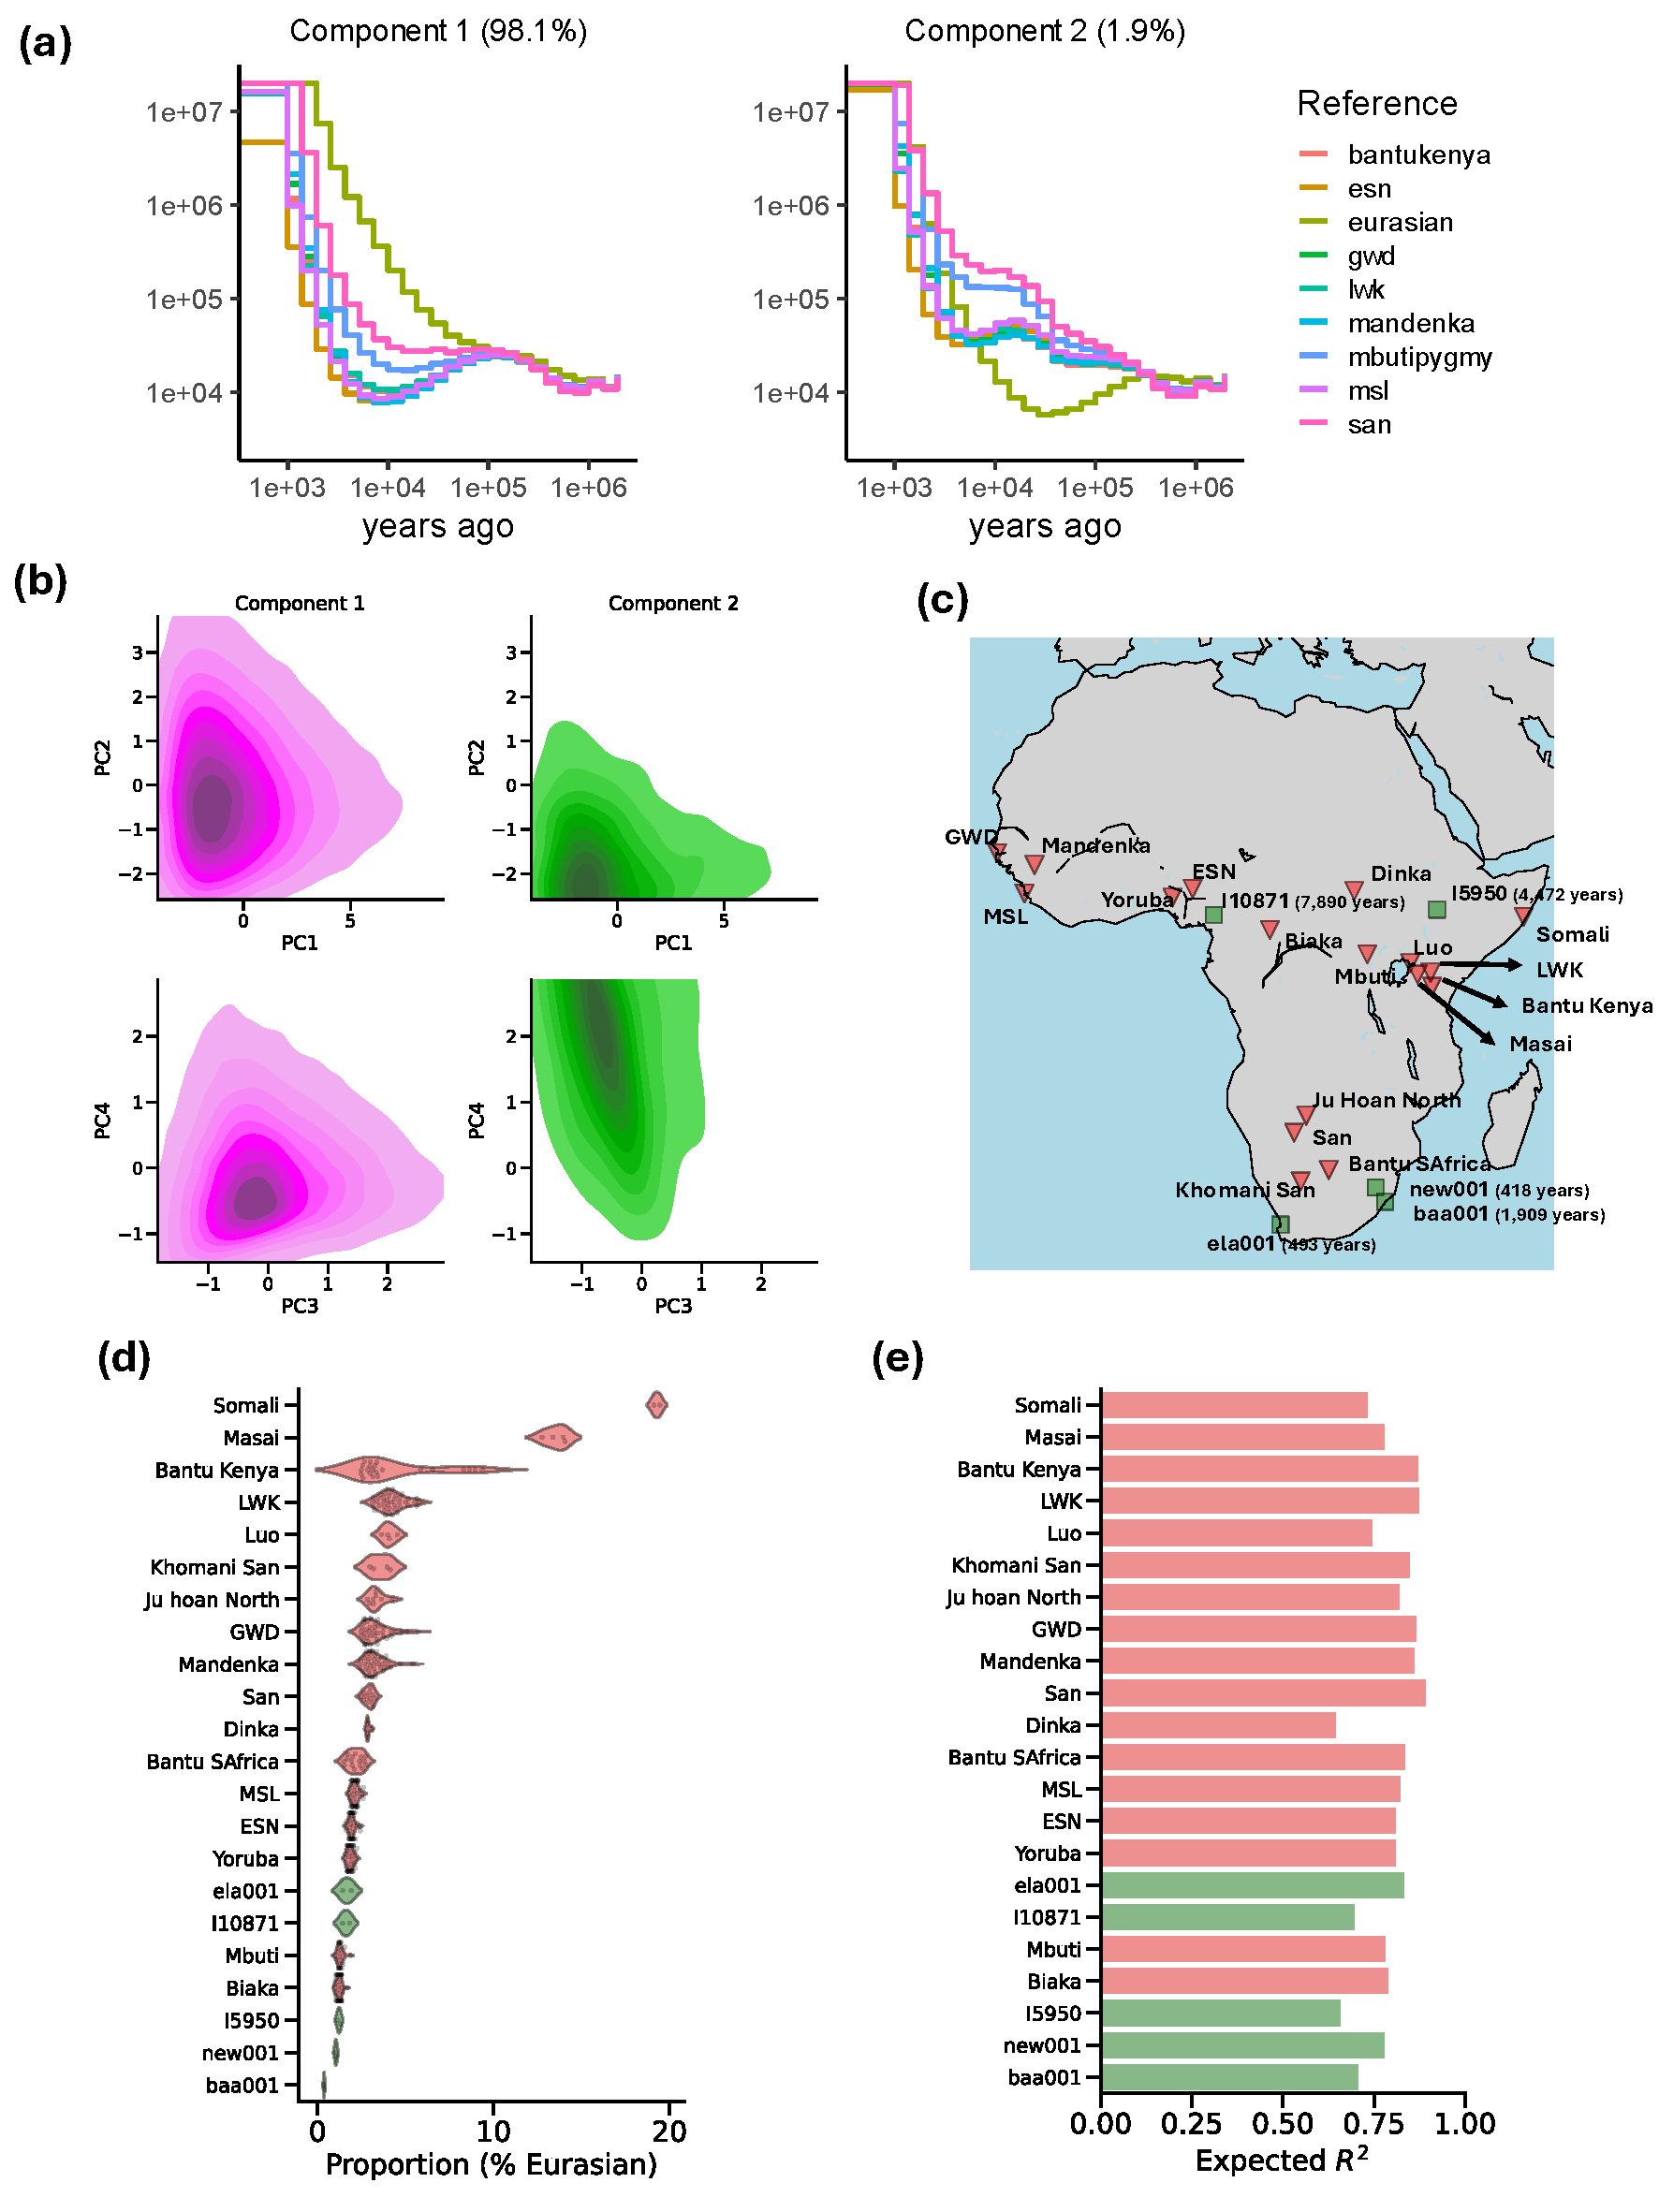
\includegraphics[width=\linewidth]{figures/gb_bta/gb_real_bta_1.pdf}
    \captionsetup{width=\textwidth+3cm}
    \caption{
    \footnotesize
    \textbf{Finding Eurasian-like ancestry in sub-Saharan Africans.} (a) Inferred inverse coalescence rates and proportions when decomposing Yorubans: each line represents inverse coalescence rate profiles with a reference population. (b) PCA visualization of the coalescence count and opportunity matrix derived from the genealogies plotted separately for each component. (c) Map of the African samples analyzed with red inverted triangles corresponding to modern samples in HGDP, $1{,}000$GP and SGDP, and green squares for 5 ancient African samples (with their estimated sampling ages in brackets). (d) Proportion of Eurasian-like ancestry and (e) Expected coefficient of determination across all African populations analyzed. The PCA visualization in (b) is based on a KDE plot with a threshold of 0.05, and binary local ancestry estimates are obtained by thresholding the inferred posteriors at 0.5. Individual data-points overlaid on the violin plots. 
    }
    \label{fig:gb_bta_1}
\end{figure}

\clearpage

\subsection{Dating the admixture event}
\label{sec:ch3-gb-bta-dating}

We dated these admixture events using coancestry curves derived from the local ancestry inferred by GhostBuster. To capture population-specific variation, we estimated admixture dates separately for each African population. However, for single-sample individuals, we could not apply the pseudo-individual normalization method described in Section \ref{sec:ch2-gb-coancestry}, which is critical for addressing population-specific drift and ensuring unbiased admixture date inference. We therefore do not report admixture dates for ancient individuals and the Somali population.

We fit the coancestry curves using three models: a single-date admixture model, a two-date admixture model, and a continuous admixture model with a constant migration rate. Our analysis revealed that a single admixture date did not adequately fit the coancestry curves for several African populations, as indicated by the visual fit of the coancestry curves and significant in-sample log-likelihood difference between the single-date and two-date admixture models ($> 20 \times \text{difference in number of parameters}$). This finding suggests a more complex genetic history (see Figure \ref{fig:gb_bta_3}a-c). Both the two-date and continuous admixture models provided an improved fit to the coancestry curves, as measured by the log-likelihood of the least squares fit. Notably, the two-date admixture model outperformed the continuous migration model in 14 out of 16 African populations (see Figure \ref{fig:gb_bta_3}d).

\begin{figure}[h!]
    \centering
    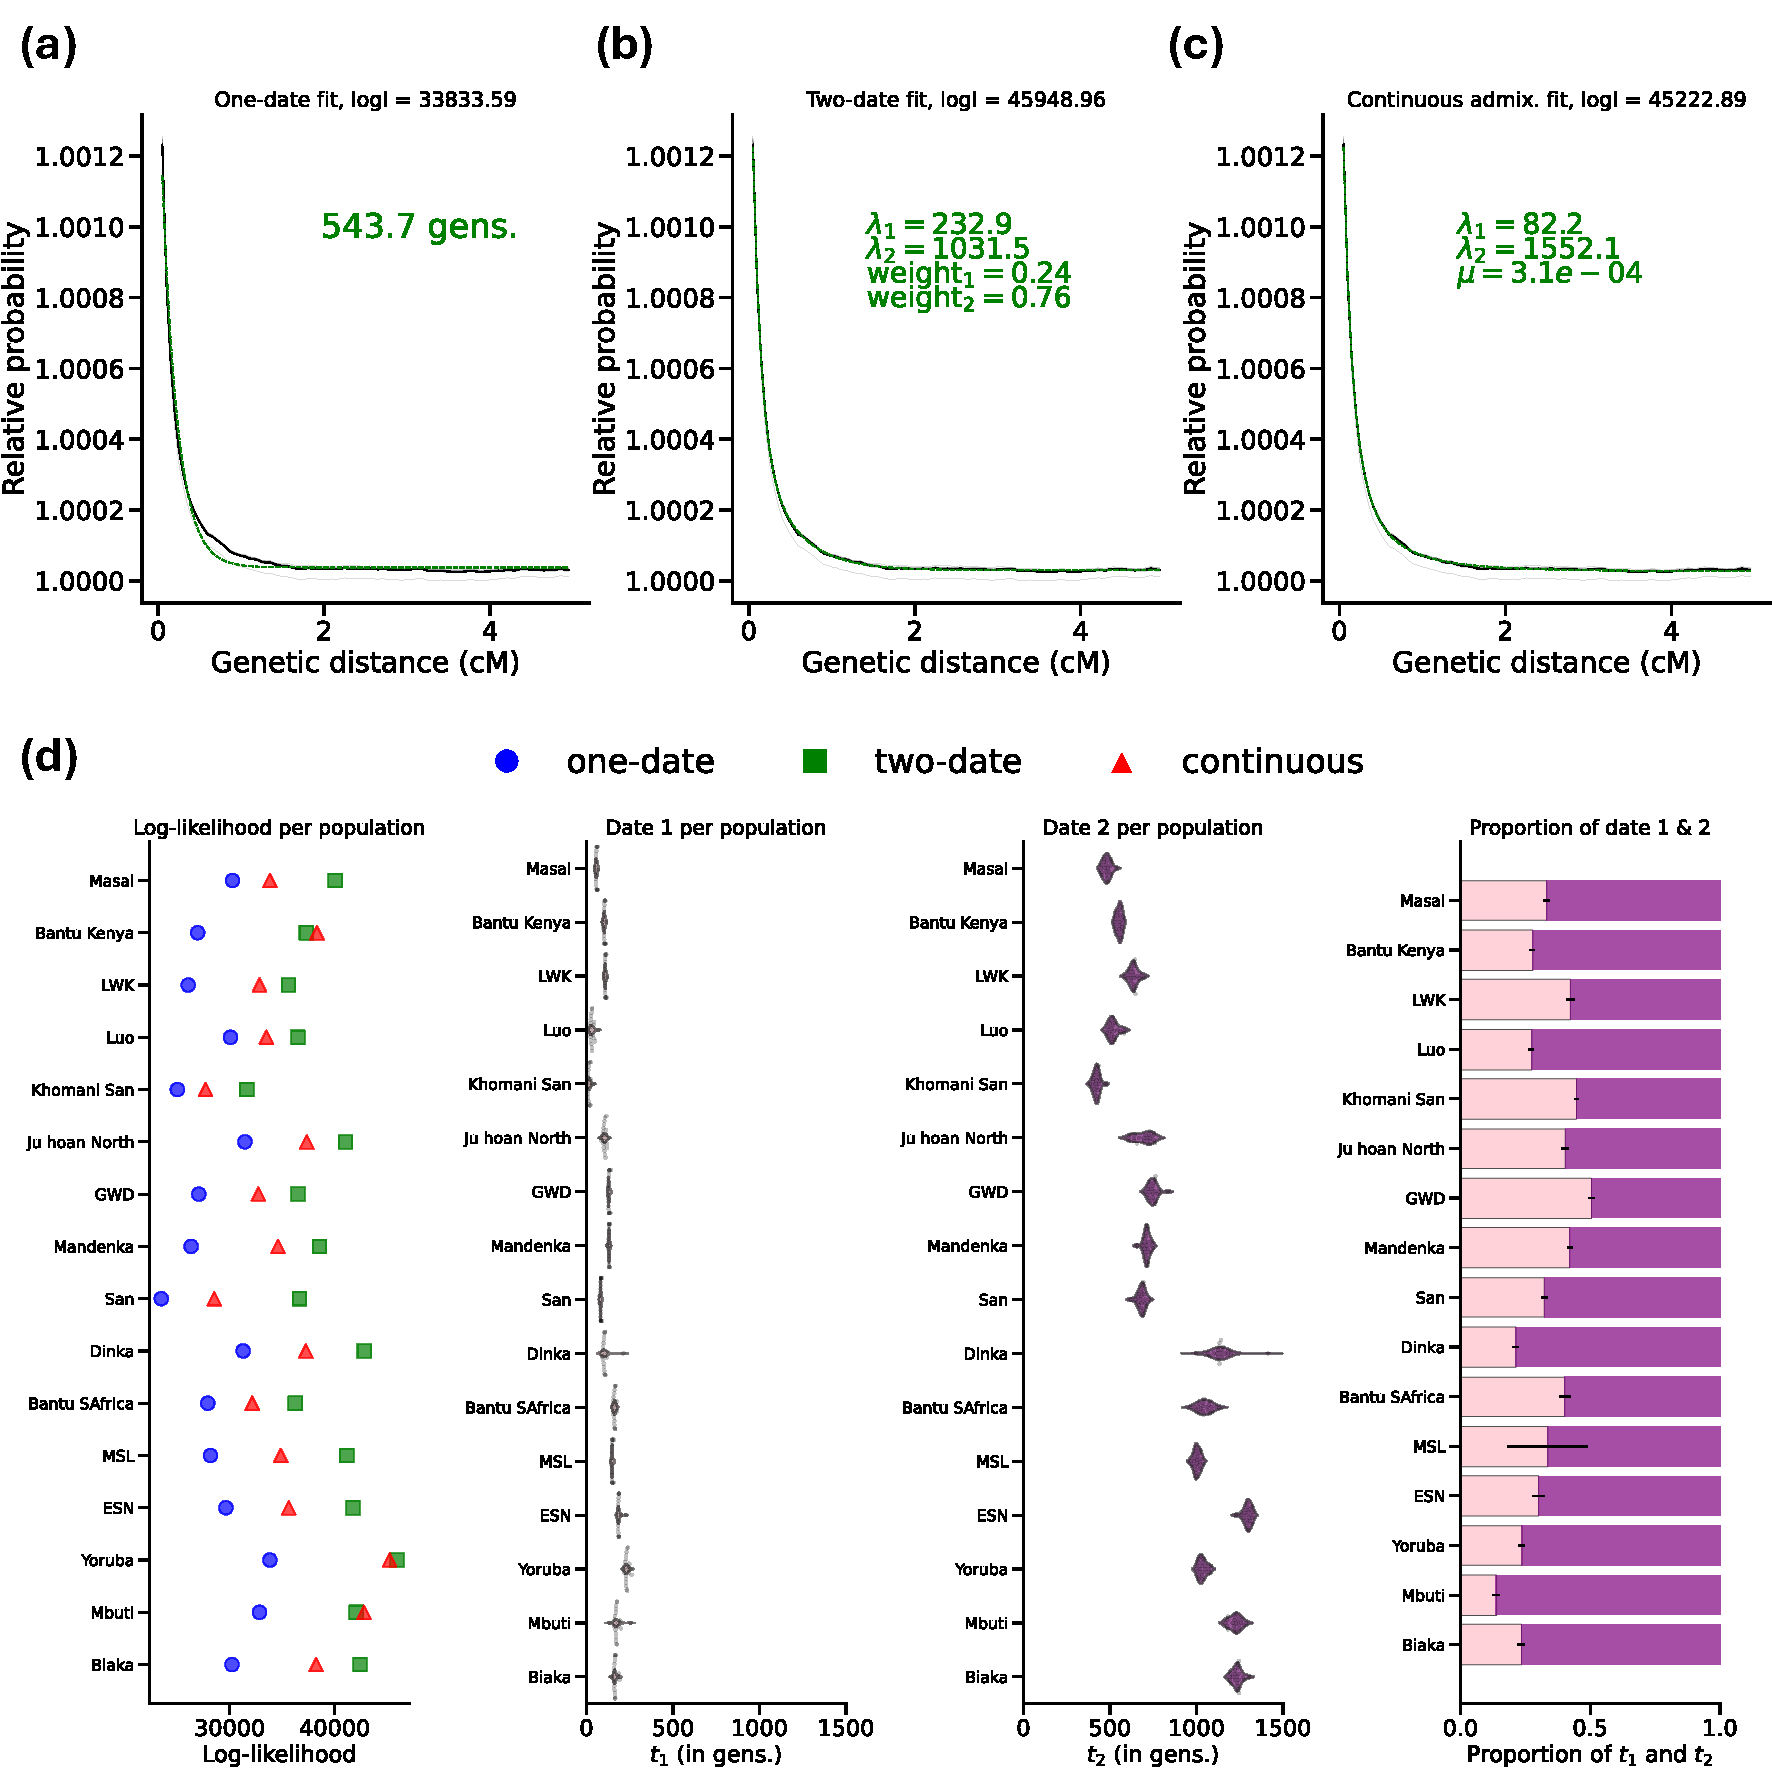
\includegraphics[width=\linewidth]{figures/gb_bta/gb_real_bta_3.pdf}
    \captionsetup{width=\textwidth+3cm}
    \caption{
    \footnotesize
    \textbf{Dating the Eurasian-like ancestry in sub-Saharan Africans.} Coancestry curves and (a) one-date admixture model fit, (b) two-date admixture model fit and (c) constant migration rate continuous admixture model fit for Yorubans. (d) Per-population least squared log-likelihood corresponding to various admixture models along with the admixture dates and weights inferred using two-date admixture model. The log-likelihood values are aggregated across $20$ jackknife runs. Populations are sorted based on highest to lowest proportion of Eurasian-like ancestry, pink represents the younger admixture date and purple represents the older admixture date in (d). Individual data-points overlaid on the violin plots. Admixture dates in the plot are in generations.
    }
    \label{fig:gb_bta_3}
\end{figure}

The two admixture dates exhibited considerable variation across geographic regions. In East African populations such as the Luhya (LWK), Bantu Kenya, Masai, and Luo, the more recent admixture event occurred $\leq 3{,}000$ years ago. In contrast, for West and Central African populations, including the Mende (MSL), Gambian (GWD), Mandenka, Esan (ESN), Yoruba, Mbuti, and Biaka, the recent admixture event is estimated to have occurred between $3{,}000$ and $7{,}000$ years ago. South African populations exhibited intermediate admixture dates ranging from $400$ to $4{,}500$ years ago, with the Khomani San showing the most recent admixture event at approximately $400$ years ago. The older admixture event dates were at least $15{,}000$ years old, ranging from $15{,}000$ to $35{,}000$ years across different African populations. Population-specific admixture dates and contributions are summarized in Figure \ref{fig:gb_bta_3}d and Table \ref{tab:gb_bta_admix_dates}. It is important to note that these admixture dates have not been adjusted for potential inaccuracies in the recombination map, as reliable error estimates were unavailable. This limitation may introduce a downward bias in the dating of the older admixture event \cite{sankararaman2012date}.

Given the distinct dates of these two admixture events, we perform separate validation analyses for each. To differentiate between the events, we first calculate the segment length of Eurasian ancestry segments by applying a threshold to the local ancestry posterior at \(50\)\%, then combining adjacent matching ancestry segments. Next, we estimate the posterior probability that a segment belongs to either the younger (typically in the last $10{,}000$ years) or older (typically between $15{,}000$ to $35{,}000$ years) admixture event for each population, using segment length as the determining factor. In particular, we use the admixture dates and proportions as inferred using per-population coancestry curve dating to assign this posterior. Given the assumption that segment lengths follow an exponential distribution conditioned on the admixture time, we proceed with the following model, given segment length $L$, admixture times $t_{\text{younger}}$ and $t_{\text{older}}$ and priors $p_{\text{younger}}$ and $p_{\text{older}}$ from coancestry curve dating:

\begin{align}
    \text{\textbf{Likelihood:} \vspace{2mm}} & \mathbb{P}(L | t) = t e^{-t * L} \nonumber \\
    \text{\textbf{Prior:} \vspace{2mm}} & \mathbb{P}(t = t_{\text{younger}}) = p_{\text{younger}}  = 1 - p_{\text{older}} \nonumber \\
    \text{\textbf{Posterior:} \vspace{2mm}} & \mathbb{P}(t = t_{\text{younger}} | L) = \frac{\mathbb{P}(L | t_{\text{younger}}) \cdot p_{\text{younger}}}{\mathbb{P}(L | t_{\text{younger}}) \cdot p_{\text{younger}} + \mathbb{P}(L | t_{\text{older}}) \cdot p_{\text{older}}} \nonumber \\
    & \mathbb{P}(t = t_{\text{older}} | L) = \frac{\mathbb{P}(L | t_{\text{older}}) \cdot p_{\text{older}}}{\mathbb{P}(L | t_{\text{younger}}) \cdot p_{\text{younger}} + \mathbb{P}(L | t_{\text{older}}) \cdot p_{\text{older}}}
\end{align}

We estimate the posterior probability of each position in the local ancestry belonging to either the younger or older admixture event. By combining these posterior estimates with GhostBuster's initial local ancestry inference, we obtain the probabilities that each segment represents either a younger or older Eurasian ancestry. Additionally, we construct histograms reflecting the segment length distribution for each population analyzed (see Figure \ref{fig:gb_segment_histogram}). In subsequent sections, we demonstrate that these younger and older Eurasian segments differ in their mutational signatures and levels of Neanderthal enrichment. We hypothesize that the younger Eurasian segments correspond to a back-to-Africa migration originating from Eurasia, while the older segments likely represent an ancient admixture event between African groups -- those who likely remained in Africa and those who migrated out of Africa. For much of the analysis in subsequent subsections, we focus primarily on the younger segments to highlight their distinct properties relative to the older segments. However, a detailed analysis of the older admixture segments is conducted in further Section \ref{sec:ch3-gb-deep}.

% \clearpage

\subsection{Eurasian ancestry explains the Neanderthal ancestry in Africans}

Previous research has shown that modern Africans carry small amounts of Neanderthal ancestry in their genomes, likely due to a back-migration event from Europe \cite{chen2020identifying, bergstrom2020insights, wang2013apparent, hollfelder2017northeast}. We look for this Neanderthal ancestry as a way to validate the Eurasian segments identified in our analysis. Specifically, we used GhostBuster to detect Neanderthal ancestry in African individuals by jointly analyzing genealogies inferred from both modern African samples and ancient samples, including three Neanderthal genomes from the Altai, Chagyrskaya, and Vindija caves.

Our analysis focused on coalescence events that occurred between $50{,}000$ and 2 million years ago, partitioning this time frame into 20 epochs on a logarithmic scale. To specifically detect Neanderthal segments rather than other ancient events, we restricted the analysis to coalescence events with sequenced Neanderthals only, ignoring the rest of the tree. We began by setting the cluster coalescence rates to genome-wide coalescence rates observed between sequenced Neanderthals themselves and the target African populations. Using these predefined coalescence rates, we employed the EM algorithm to estimate admixture proportions, admixture time, and local ancestry across the sample. In the final iteration of the EM algorithm, we update the coalescence rates based on the inferred local ancestry instead of using the pre-specified genome-wide coalescence rates. This adjustment fine-tunes the estimates to account for differences between the Neanderthal sources that contributed ancestry to Africans and the sequenced Neanderthals, allowing us to obtain unbiased and accurate estimate of Neanderthal local ancestry in African genomes. 

To validate our approach for detecting Neanderthal ancestry, we first estimated Neanderthal ancestry in Eurasians, recovering approximately $1$–$2$\% across six modern Eurasian groups (see Figure \ref{fig:gb-bta-nea-eurasians}). These proportions align with prior findings \cite{prufer2014complete,skov2020nature}. East Asian populations exhibited approximately $20$\% higher Neanderthal ancestry, with an average of $1.5$\%, compared to South Asians and Europeans, which showed about $1.25$\% Neanderthal ancestry -- consistent with previous studies \cite{meyer2012high,iasi2024neandertal}. Furthermore, we observed little to no Neanderthal ancestry in genomic regions previously identified as ``archaic deserts'' \cite{sankararaman2016combined,vernot2016excavating} (see Figure \ref{fig:gb-bta-nea-eurasians}d).  It is important to note our approach circumvents the need for un-admixed reference samples or identity-by-descent (IBD) segments with Neanderthals, and utilizes the entire coalescence history with sequenced Neanderthal directly, making it more robust and powerful for finding Neanderthal ancestry in Africans.  

We found that African samples from the HGDP+$1{,}000$GP dataset exhibit approximately \( 0.004\% \) to \( 0.056\% \) Neanderthal ancestry, with the lowest levels observed in Mbuti individuals and the highest levels in Bantu Kenyans, among the populations analyzed. Figure \ref{fig:gb_bta_nea}a shows the inverse coalescence rates for Neanderthal ancestry in Yoruba (as a representative population). Our analysis revealed a strong correlation between the genome-wide Neanderthal proportion and the Eurasian-like ancestry proportion inferred with GhostBuster, yielding a correlation \( R^2 = 0.51 \). To examine Neanderthal ancestry correlations associated with the younger and older admixture events, we fitted a joint regression model to predict Neanderthal ancestry proportion based on the proportions of younger and older Eurasian ancestry within individuals. The younger Eurasian ancestry proportion had a slope of \(1.22\%\), whereas the older Eurasian ancestry showed a slope of \(0.67\%\). These slopes represent the increase in Neanderthal ancestry per unit increase in Eurasian-like ancestry, effectively quantifying the proportion of Neanderthal ancestry within these Eurasian segments. The joint regression also inferred an intercept not significantly different from $0$ at $0.009$\%. This suggests a probable absence of Neanderthal ancestry in non-Eurasian-like segments and highlights a disparity in Neanderthal ancestry between the two Eurasian-like segments identified in Africa (see Figure \ref{fig:gb-bta-nea-supp2}). 
%It is also possible the older admixture ancestry lacks Neanderthal ancestry completely due to presence of short segments corresponding to younger admixture event misclassified as older admixture event.

At the local ancestry level, we defined the enrichment of Neanderthal ancestry within Eurasian segments as the mean local ancestry posterior for Neanderthal ancestry in Eurasian segments (determined by a local ancestry threshold of 0.5) divided by the mean posterior in non-Eurasian segments. Under a model with no correlation between Neanderthal and Eurasian-like ancestry in Africa, this enrichment should be close to unity. However, we observed a \(21.9\times\) enrichment of Neanderthal ancestry within Eurasian segments compared to non-Eurasian segments (see Figure \ref{fig:gb_bta_nea}b). Further stratification of Eurasian segments by length showed even higher enrichment for longer segments and lesser enrichment for shorter segments: \( 31.4\times \) for segments longer than \(0.5\)cM, \( 23.1\times \) for segments between \(0.2\) and \(0.5\)cM, \( 11.3\times \) for segments between \(0.1\) and \(0.2\)cM, and \( 4.3\times \) for segments shorter than \(0.1\)cM. 

The disparity in estimated coefficients for older and younger admixture in Figure \ref{fig:gb-bta-nea-supp2}, combined with reduced enrichment in shorter segments, suggests the possibility that Neanderthal ancestry is entirely absent from the older admixture event and the reduced signal is only driven by misassignment of segments originating from the more recent event to the older event. To obtain more robust estimates of Neanderthal local ancestry while minimizing false-positive rates, we recalculated Neanderthal ancestry in Africans by masking non-Eurasian-like segments and only using the Eurasian-like segments during coalescence rate inference. This masking produced genome-wide proportions of Neanderthal ancestry that were comparable to the original run without masking (paired t-test, $p=0.18$).

We dated the admixture event using Eurasian segments that specifically contained at least one Neanderthal segment. This analysis aimed to determine whether Neanderthal ancestry was present in both the younger and older Eurasian segments. If a date exceeding $20{,}000$ years is detected, it would indicate that the older Eurasian segments also carried Neanderthal ancestry. Conversely, detecting only more recent admixture dates would suggest that Neanderthal ancestry arrived exclusively through the more recent admixture event. We constructed coancestry curves using hard-called local ancestry, where Eurasian-like segments with Neanderthal ancestry (posterior probability $\geq 0.1$) at at least one position were assigned a value of 1, while all other regions, including Eurasian-like segments without Neanderthal ancestry, were assigned a value of 0. We then fit multiple admixture models to the generated coancestry curves. Our analysis revealed that a single admixture date provides an adequate (in-sample log-likelihood difference between single- and two-date admixture models $< 2 \times \text{difference in number of parameters}$, see Figure \ref{fig:gb-bta-nea-supp3}) fit for most African populations, with some exceptions. For instance, populations such as Bantu Kenya from East Africa fit better with a two-admixture-date model. Similarly, West African populations like Gambian (GWD) and Mende (MSL) also showed a slight improvement with a two-admixture-date model, though these estimates were more noisy (see Figure \ref{fig:gb-bta-nea-supp3}). The admixture dates corresponding to both single- and two-date models for some populations ranged approximately from 4,000 to 10,000 years ago (see Figure \ref{fig:gb_bta_nea}c-d). These admixture dates fall within the range of the younger admixture dates inferred previously in Section \ref{fig:gb_bta_3}, and are not consistent with the older admixture date. This suggests that the older admixture date, which occurred approximately $15{,}000$ - $35{,}000$ years ago, did not carry Neanderthal ancestry. Furthermore, admixture dates varied based on the present-day geographic location of samples. West African populations, such as Yoruba and Esan, exhibited the oldest admixture dates, approaching $10{,}000$ years ago -- aligning with the green Sahara period \cite{tierney2017rainfall, larrasoana2013dynamics} and well before the expansion of Bantu-speaking peoples. Central African hunter-gatherers, including Mbuti individuals, exhibit minimal Neanderthal ancestry, leading to noisier coancestry curve dating and were therefore excluded from the main figure. More detailed results, including the dating of Neanderthal ancestry in Mbuti individuals, can be found in Figure \ref{fig:gb-bta-nea-supp3}. These findings suggest that the Neanderthal ancestry present in Africans is predominantly associated with the younger admixture event, which occurred during the Holocene, starting shortly after the end of the last Ice Age.

To further validate our hypothesis that the older Eurasian segments do not carry substantial Neanderthal ancestry, we analyzed the mean posterior probability of Neanderthal ancestry as a function of segment length. We compared the empirical estimates of mean Neanderthal posterior probabilities to theoretical predictions from a two-date admixture model, under the assumption that only the younger admixture event contributes Neanderthal ancestry. The theoretical model is defined as follows:
\begin{align}
    P ( L \leq l | \text{model}_{\text{younger}}) &= 1 - e^{-lt_{\text{younger}}} \nonumber \\
    P ( L \leq l | \text{model}_{\text{older}}) &= 1 - e^{-lt_{\text{older}}} \nonumber \\
    P ( \text{Neanderthal} | \text{model}_{\text{younger}}) &= \alpha \nonumber \\
    P ( \text{Neanderthal} | \text{model}_{\text{older}}) &= 0 \nonumber \\
    P ( \text{model}_{\text{younger}}) = 1 - P ( \text{model}_{\text{older}}) &= p_{\text{younger}}
\label{eq:gb_nea_segm_1}
\end{align}
where, $\text{model}_{\text{younger}}$ and $\text{model}_{\text{older}}$ correspond to Eurasian-like ancestry in Africans derived from the younger and older admixture events, respectively. Here, $\alpha$ represents the proportion of Neanderthal ancestry in the Eurasian source population contributing to the younger admixture event; $t_{\text{younger}}$ and $t_{\text{older}}$ are the admixture dates, and $p_{\text{younger}}$ is the proportion of ancestry contributed by the younger admixture event. These parameters are estimated using the coancestry curves presented in Section \ref{sec:ch3-gb-bta-dating}. Based on the Equation \ref{eq:gb_nea_segm_1}, the probability of Neanderthal ancestry conditioned on segment length can be expressed as:
\begin{align}
    P( \text{Neanderthal} | L \leq l) = \frac{\alpha p_{\text{younger}} (1 - e^{-lt_{\text{younger}}})}{p_{\text{younger}} (1 - e^{-lt_{\text{younger}}}) + (1 - p_{\text{younger}}) (1 - e^{-lt_{\text{older}}})}
\end{align}

We estimated confidence intervals for the theoretical models by incorporating uncertainties in coancestry dating. Our results showed that the theoretical model, assuming no Neanderthal ancestry from the older admixture event, fit the empirical data well across several populations (see Figure \ref{fig:gb-bta-nea-supp}). This finding further supports the hypothesis that the older admixture event did not contain substantial Neanderthal ancestry. 
% However, some populations, including the San, Mbuti, and Yoruba, deviated from the theoretical curves. These discrepancies suggest the possibility of multiple sources of Neanderthal ancestry, including contributions from the older admixture event for some of these populations.

Finally, we analyzed Neanderthal content in ancient African samples, finding \( 0.026\% \) and \( 0.017\% \) Neanderthal ancestry in ela001 ($493$ years) and new001 ($418$ years) individuals respectively, and \( 0.01\% \) in the $1{,}900$-year-old Ballito Bay individual (baa001). In contrast, we detected no Neanderthal ancestry (\(<10^{-9}\%\)) in ancient samples from the Mota Cave ($4{,}472$ years) and Cameroon ($7{,}890$ years). This again suggests that the younger admixture event which might be missing in Mota and Cameroon individuals contributed Eurasian-like ancestry with detectable Neanderthal ancestry, whereas the older admixture event might be associated with reduced or no Neanderthal ancestry.

\begin{figure}[h!]
    \centering
    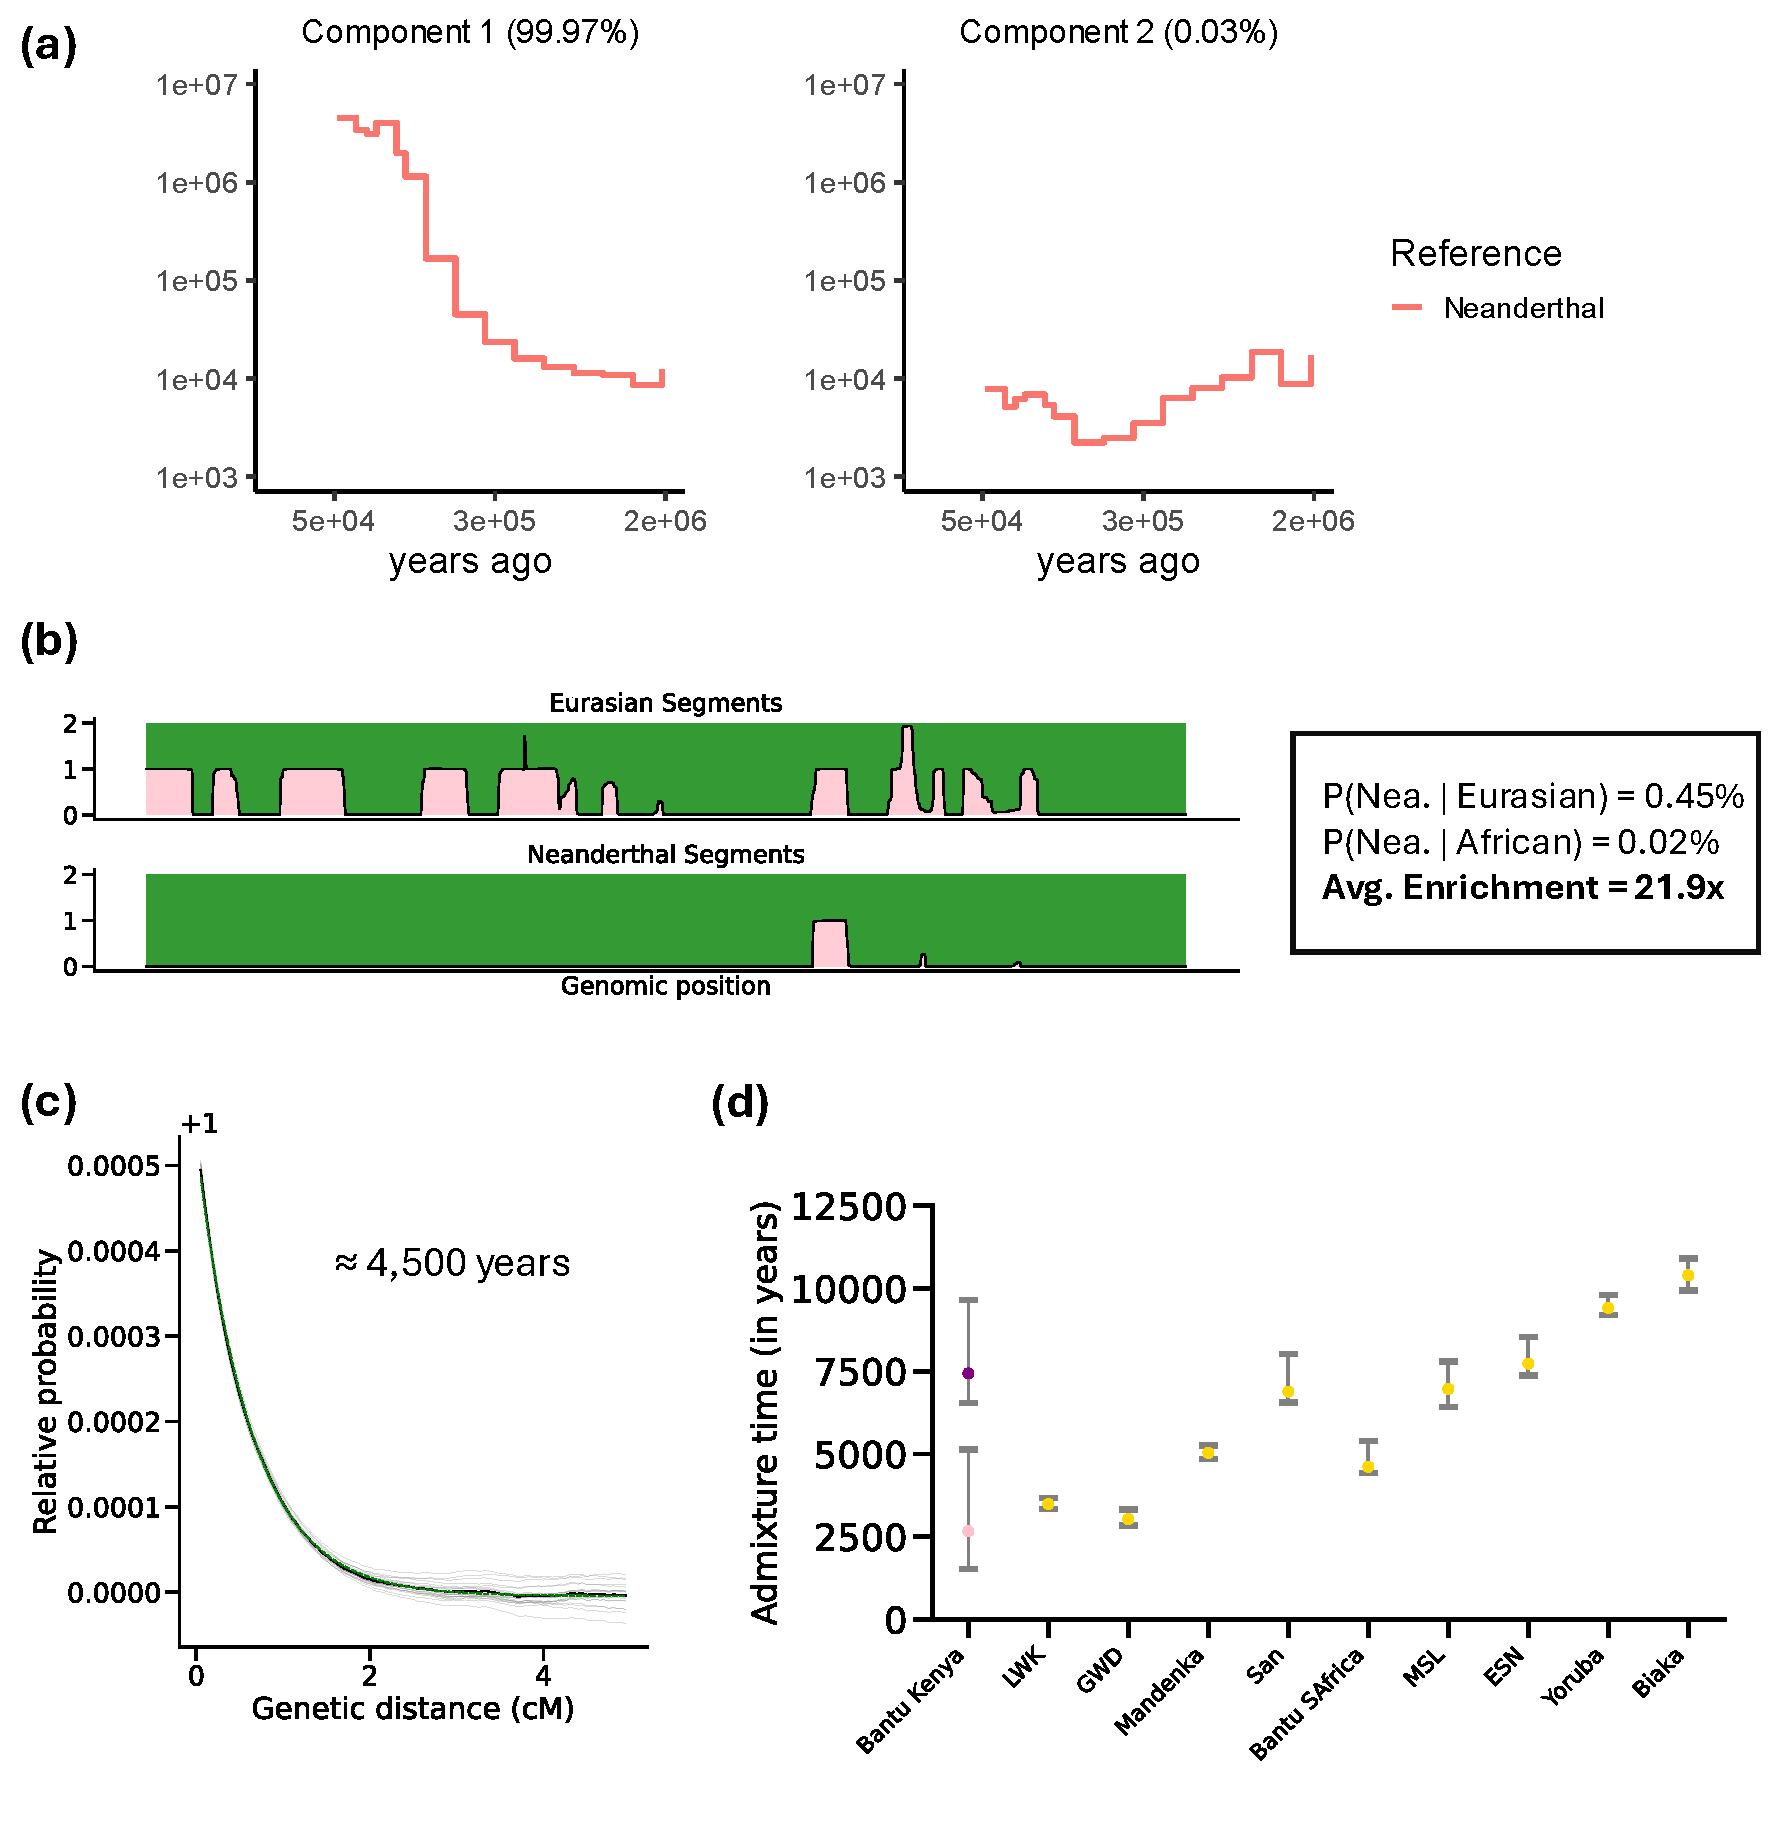
\includegraphics[width=\linewidth]{figures/gb_bta/gb_real_bta_6.pdf}
    \captionsetup{width=\textwidth+3cm}
    \caption{
    \footnotesize
    \textbf{Eurasian ancestry explains the Neanderthal ancestry in Africans.} (a) Inferred inverse coalescence rates and proportions for Neanderthal ancestry in Yorubans: the line represents the inverse coalescence rate profiles with sequenced Neanderthals. (b) Sample HGDP01405 showing a 20 Mb region enriched for Neanderthal ancestry, overlapping Eurasian-like segments. The average enrichment is calculated as the ratio of the mean posterior probability of Neanderthal ancestry in Eurasian segments, $P(\text{Nea} \mid \text{Eurasian})$, to the mean posterior probability in African segments, $P(\text{Nea} \mid \text{African})$. (c) Coancestry curve showing the normalized joint probability and single admixture date fit for Eurasian segments carrying Neanderthal ancestry, averaged across all African samples analyzed. (d) Admixture dates derived from coancestry curves generated by Eurasian segments carrying Neanderthal ancestry for each population. For Bantu Kenya a two-date admixture model fit is shown, as it better explains the coancestry patterns. More detailed results are provided in Figure \ref{fig:gb-bta-nea-supp3}. Grey lines in (c) and error bars in (d) represent jackknife estimates and 95\% confidence intervals around the mean. For panel (d) single date admixtures shown in golden, whereas two date admixtures shown in pink and purple. Results derived from HGDP+$1{,}000$GP+aDNA+archaic genealogies.}
    \label{fig:gb_bta_nea}
\end{figure}


\clearpage

\subsection{Mutational profiles validate Eurasian segments in Africans}
\label{sec:ch3-gb-bta-mutational}

Evidence suggests that human mutation rates have evolved over short time scales and independently across different populations \cite{harris2015evidence, harris2017rapid}. One notable example is the TCC to TTC mutation, which occurs at up to twice the rate in West Eurasian groups compared to East Asians or Africans. Another example is GC-biased gene conversion (GCbGC) \cite{duret2009biased}, which preferentially selects GC alleles (termed ``strong'') over AT alleles (termed ``weak''). GCbGC is influenced by factors such as population size and recombination hotspots: populations with larger effective population sizes or fewer bottlenecks exhibit higher rates of weak to strong mutations than populations with reduced population sizes. Figure \ref{fig:gb_bta_ws_vs_sw} illustrates the evolution of weak to strong mutations relative to strong to weak mutations across various continental populations.

To investigate this within the context of the back-migration event, we define the normalized mutation rate similar to the Relate \cite{speidel2019method} paper for a specific mutation type (example, TCC to TTC, or weak to strong) in a given population. This normalized mutation rate (NMR) is calculated as the ratio of the number of mutations of that specific type that have arisen in the population to the number of mutations of all other types that have arisen in the same population. Formally, this is expressed as:
\begin{equation}
    \text{NMR}_{\text{pop, type}} = \frac{\sum_{mut} \mathbbm{1}(mut \in \text{type}) \, N_{mut, pop}}{\sum_{mut} \mathbbm{1}(mut \notin \text{type}) \, N_{mut, pop}}
\end{equation}
where, $\sum_{mut}$ sums all the mutations in the genealogy, $N_{mut, pop}$ counts the number of individuals belonging to population `pop' carry the mutation `mut'. We further stratify mutation rates by allele age, dividing them into 10 epochs ranging from $1{,}000$ years to 1 million years. To facilitate meaningful comparisons, we further divide these normalized mutation rates (NMR) and the normalized mutation rates (NMR) in African populations:
\begin{equation}
    \text{NMRE}_{\text{pop, type}} = \frac{\text{NMR}_{\text{pop, type}}}{\text{NMR}_{\text{AFR, type}}}
\end{equation}
This measure, referred to as the Normalized Mutation Rate Enrichment (NMRE), quantifies the relative enrichment of specific mutation types in a given population compared to their normalized mutation rates in Africans. A significant deviation from unity indicates that the specific mutation type is either enriched (greater than 1) or depleted (less than 1) in the population relative to the African baseline. We examine this enrichment across various continental populations, including all non-Finnish Europeans (NFE), East Asians (EAS), South Asian (SAS) and Middle Eastern and North African (MID) groups in HGDP. Notably, we analyze the enrichment for Eurasian and non-Eurasian segments in African samples separately. To correct for mutational biases in local ancestry fitting, we down-sample Eurasian and non-Eurasian segments at each location to equalize the number of descendants in both categories. We perform $1{,}000$ chromosome-wise bootstraps to estimate the confidence interval around the normalized mutation rate enrichment. 

Examining the TCC to TTC mutation types, we observe significant enrichment not only in European, Middle Eastern, and South Asian populations but also in the Eurasian-like segments within African individuals. In Figure \ref{fig:gb-mut-tcc}a,b, this enrichment is plotted separately for Eurasian segments, conditioned on their segment lengths. Both long and short Eurasian segments in Africans exhibit significant enrichment in TCC to TTC mutations during the period from $1{,}000$ to $40{,}000$ years ago, consistent with the evolutionary trajectory of these mutations, which rose sharply around $15{,}000$ years ago and declined approximately $2{,}000$ years ago \cite{harris2017rapid}. The enrichment is particularly pronounced in longer Eurasian segments, which are more likely to be associated with the younger admixture date, peaking at approximately $2\times$ around $20{,}000$ years ago -- levels comparable to those observed in Europeans. This pattern suggests a European source as the most probable origin for the back-to-Africa migration.

%We did not detect this enrichment in Africans before due to the limited proportion of Eurasian segments in their genomes. However, by leveraging local ancestry inferred through GhostBuster, we were able to isolate and identify this enrichment, providing independent validation of the back-migration event we identified.  

\begin{figure}
    \centering
    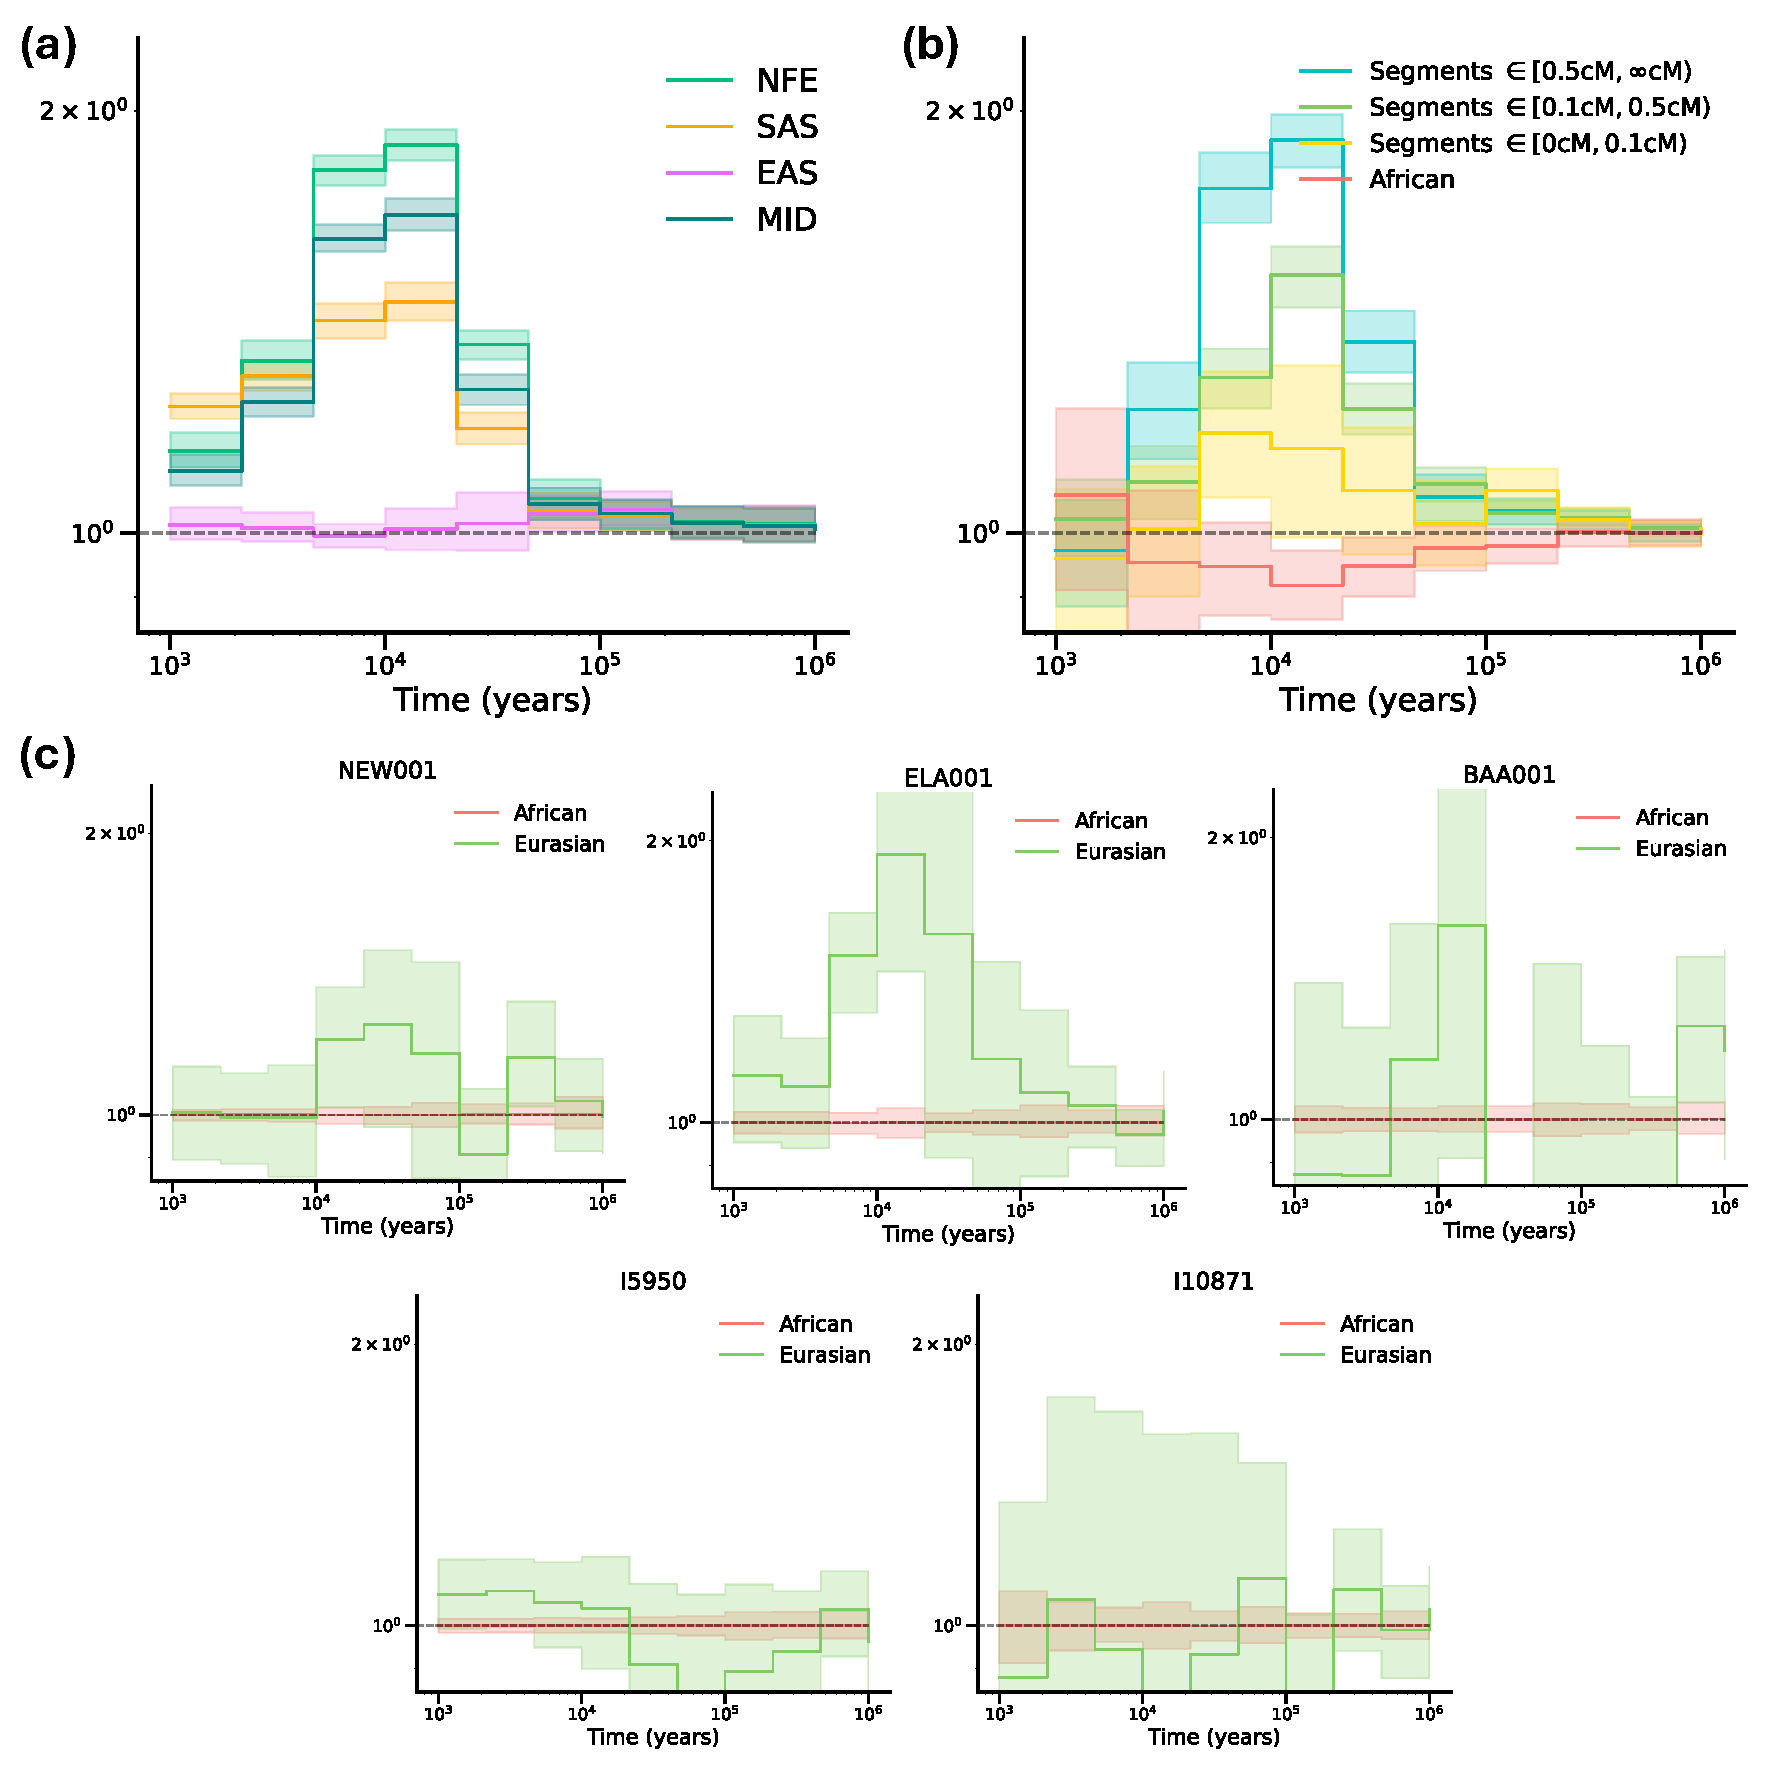
\includegraphics[width=\linewidth]{figures/gb_bta/gb_real_bta_8.pdf}
    \captionsetup{width=\textwidth+3cm}
    \caption{
    \footnotesize
    \textbf{Enrichment of TCC to TTC mutation rates in African components.} (a) Enrichment of TCC to TTC mutation rates across various continental groups, including NFE (non-Finnish Europeans), SAS (South Asians), EAS (East Asians), and MID (Middle Eastern and North African populations). (b) Enrichment of TCC to TTC mutation rates in Eurasian and non-Eurasian (African) segments in African populations. (c) TCC to TTC mutation rate enrichment in five ancient African samples, including new001, ela001, baa001, I5950, and I10871 (see population descriptions in Table \ref{tab:african_populations_2}). Shaded regions indicate 95\% confidence intervals derived from $1{,}000$ bootstrap replicates, while the dashed line represents the baseline of no enrichment. In panel (b), the Eurasian segments in Africans are further categorized based on their lengths: segments shorter than 0.1 cM, those between 0.1 and 0.5 cM, and segments longer than 0.5 cM. Results derived from HGDP+$1{,}000$GP and HGDP+$1{,}000$GP+aDNA+archaic genealogies.
    }
    \label{fig:gb-mut-tcc}
\end{figure}

We conducted this analysis across various African populations and consistently found enrichment in Eurasian segments across all groups. Populations with more recent admixture, such as the San, Bantu Kenya, and Mandenka, exhibited the highest enrichment, while those with older admixture events, such as the Mbuti, Biaka, and Yoruba, showed weaker enrichment for TCC to TTC mutations. Notably, some African populations, including the San and Bantu Kenyans, displayed empirical enrichment levels exceeding the average across all non-Finnish Europeans (see Figure \ref{fig:gb-mut-tcc-pops}). In our analysis of ancient African samples, similar enrichment patterns emerged, though with increased variability due to smaller sample sizes. We normalized mutation rates in ancient samples relative to the mutation rates in their African segments, rather than using mutation rates from modern African samples, to minimize the impact of differences in sampling times and biases associated with ancient DNA genealogy construction. We observed modest enrichment in more recent ancient samples from South Africa, whereas older samples from Mota Cave and Cameroon showed no detectable enrichment (see Figure \ref{fig:gb-mut-tcc}c). This absence of enrichment in older samples could be attributed to statistical noise when detecting TCC to TTC mutation enrichment in individual ancient samples or might indicate a lack of back-to-Africa admixture signals in these older populations.

In addition to examining the TCC to TTC mutations, we also investigated the enrichment of mutations related to weak to strong mutation types. For our analysis, we excluded CpG sites when defining weak or strong mutations. Similar to patterns observed in European, East Asian, and South Asian populations, the Eurasian segments within African genomes also showed reduction for weak to strong mutations relative to African genomes as a whole. The reduction in weak-to-strong mutations reached its peak approximately $50{,}000$–$100{,}000$ years ago, aligning with patterns observed in other Eurasian populations. Interestingly, Eurasian segments of all lengths in Africans exhibit a similar pattern of weak to strong mutation reduction, and with a slightly lower amplitude compared to that observed in Europeans and East Asians. This pattern suggests that the Eurasian-like ancestry in African genomes may have experienced an even more pronounced bottleneck than the population that initially migrated out of Africa (see Figure \ref{fig:gb-mut-ws}a,b). As with TCC to TTC enrichment, we stratified the weak to strong mutation reduction by population and ancient samples. We found consistent levels of weak to strong reduction across all modern populations and ancient samples, suggesting that both the younger and older admixture events may have undergone a population bottleneck approximately $50{,}000$–$100{,}000$ years ago (see Figure \ref{fig:gb-mut-ws}c and \ref{fig:gb-mut-ws-pops}). Finally, we present the mutation rate enrichment for Eurasian-like versus non-Eurasian-like segments in Africans across all 96 trimer mutation types, as shown in Figure \ref{fig:gb-mutational-all-bta}.

\begin{figure}
    \centering
    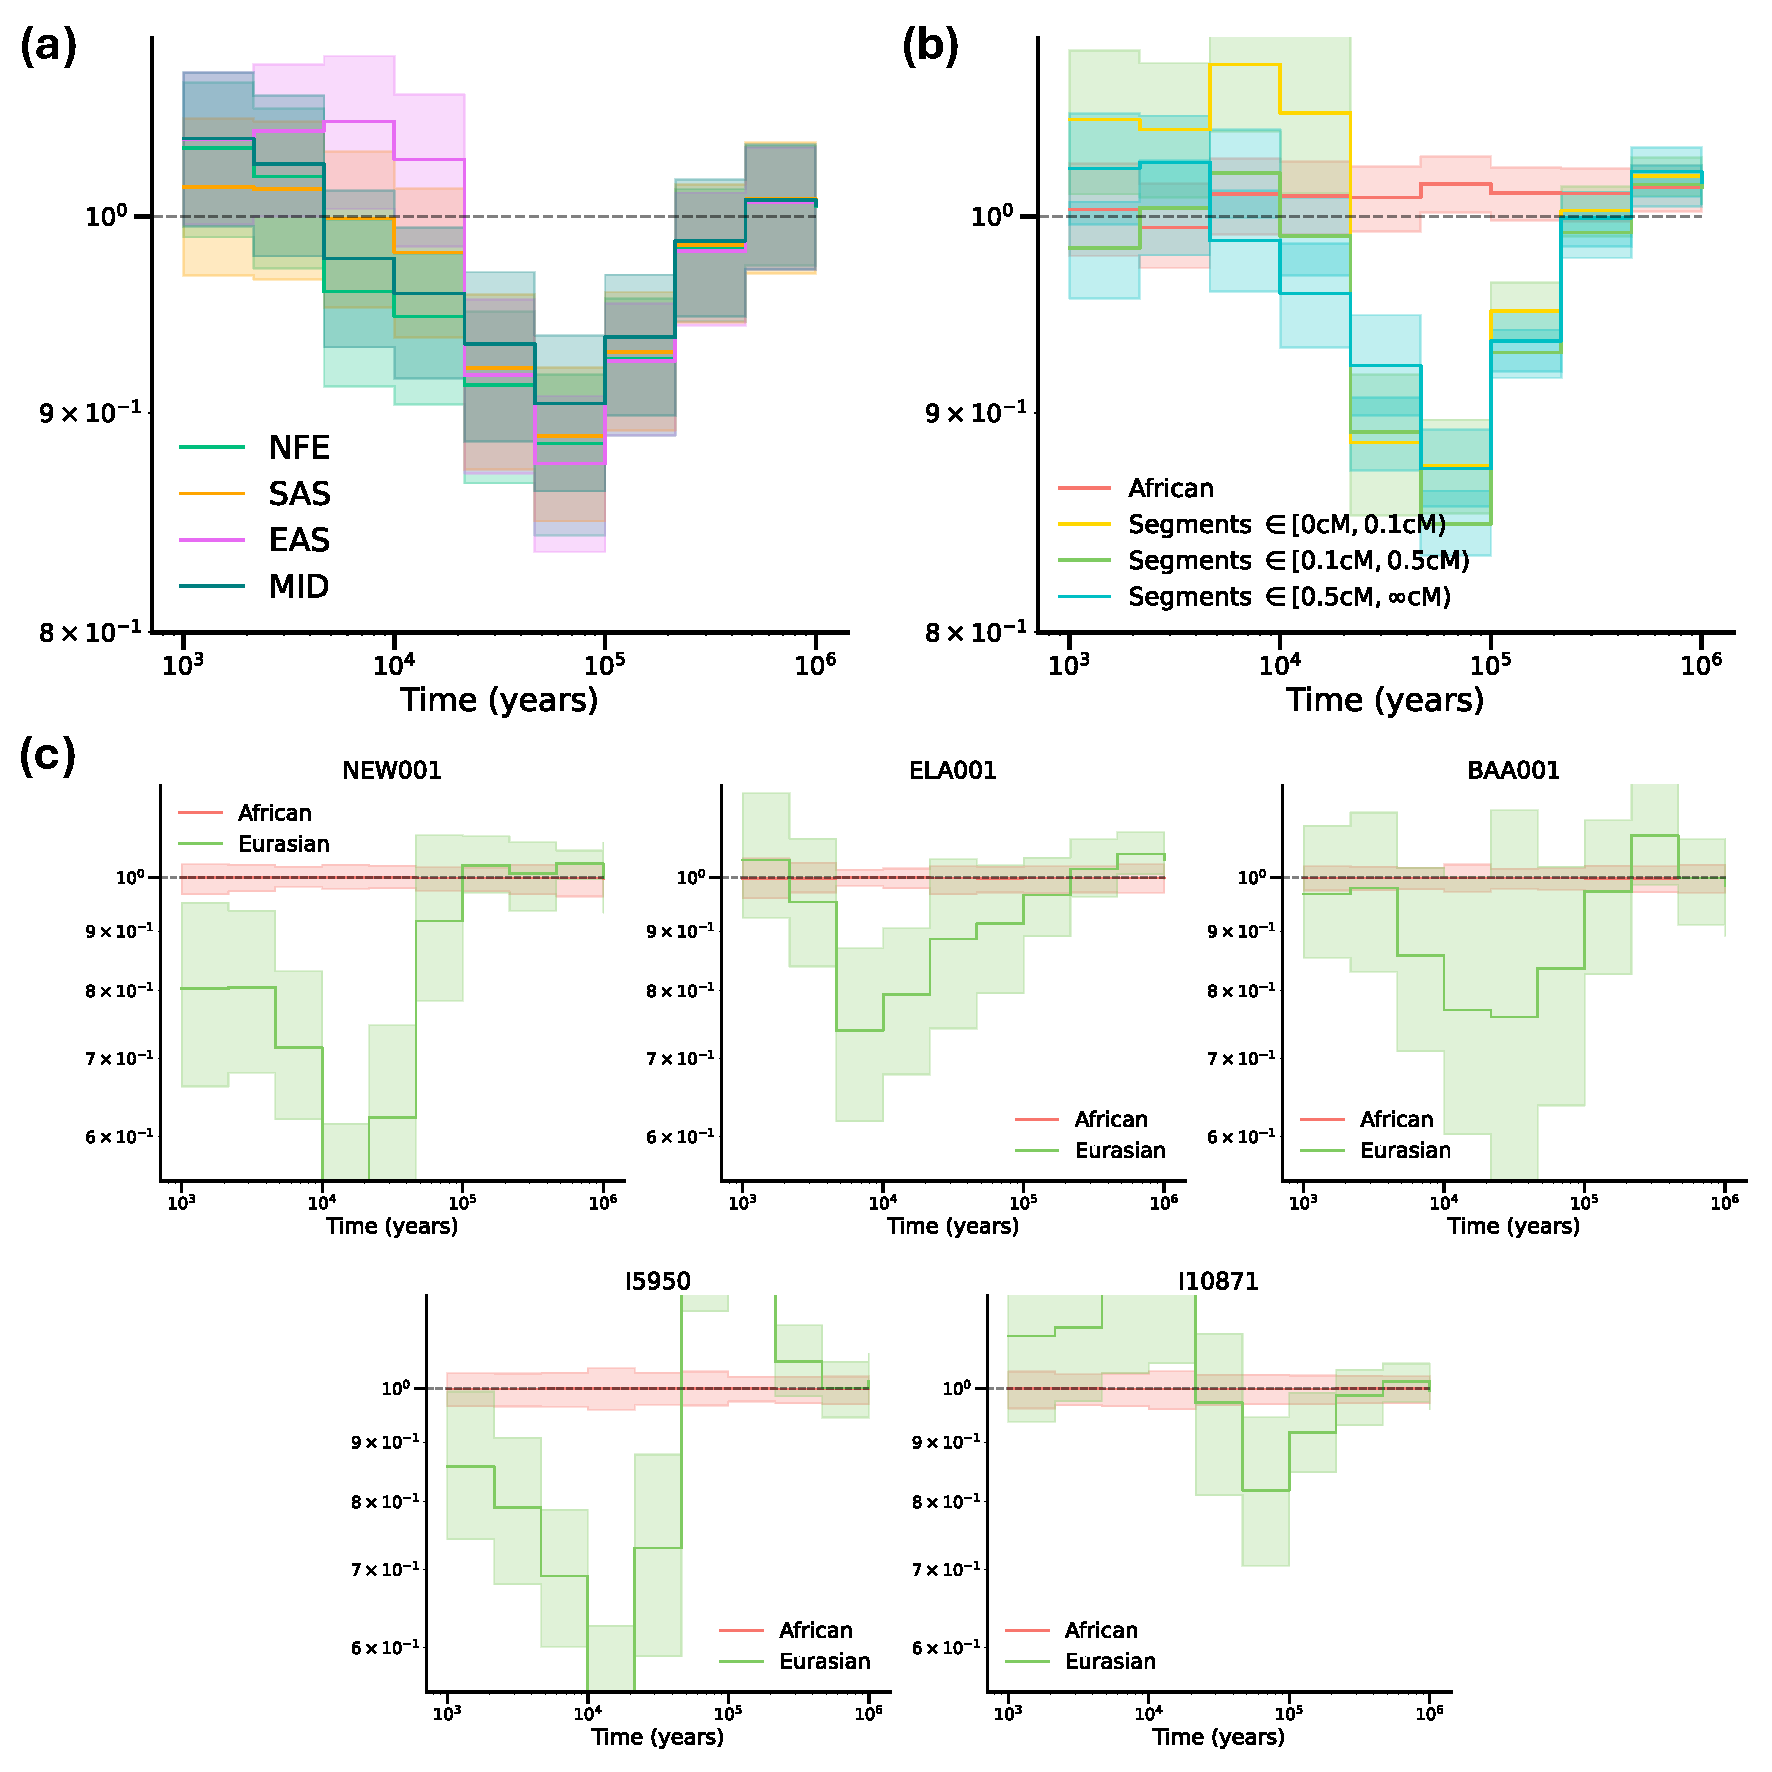
\includegraphics[width=\linewidth]{figures/gb_bta/gb_bta_real_10.pdf}
    \captionsetup{width=\textwidth+3cm}
    \caption{
    \footnotesize
    \textbf{Enrichment of weak to strong mutation rates in African components.} (a) Enrichment of weak to strong mutation rates across various continental groups, including NFE (non-Finnish Europeans), SAS (South Asians), EAS (East Asians), and MID (Middle Eastern and North African populations). (b) Enrichment of weak to strong mutation rates in Eurasian and non-Eurasian (African) segments in African populations. (c) weak to strong mutation rate enrichment in five ancient African samples, including new001, ela001, baa001, I5950, and I10871 (see population descriptions in Table \ref{tab:african_populations_2}). Shaded regions indicate 95\% confidence intervals derived from $1{,}000$ bootstrap replicates, while the dashed line represents the baseline of no enrichment. In panel (b), the Eurasian segments in Africans are further categorized based on their lengths: segments shorter than 0.1 cM, those between 0.1 and 0.5 cM, and segments longer than 0.5 cM. Results derived from HGDP+$1{,}000$GP and HGDP+$1{,}000$GP+aDNA+archaic genealogies.
    }
\label{fig:gb-mut-ws}
\end{figure}


\clearpage

\subsection{Identifying source populations for Eurasian ancestry}
\label{sec:ch3-gb-bta-source}

To characterize the admixture event and identify potential source populations contributing Eurasian-like ancestry to Africa, we calculated coalescence rates using modern samples from the HGDP+$1{,}000$GP dataset and a subset of 40 high-coverage ancient samples with estimated sampling ages less than $10{,}000$ years and sampled in Eurasia or Africa (see Table \ref{tab:gb_ancient_samples} for list of all ancient samples). For clarity, we grouped ancient samples corresponding to Neolithic Anatolian and Balkan farmers into one group, and Western Hunter-gatherers into one group. We used Colate \cite{speidel2021inferring} with the \texttt{--mode local\_ancestry} flag to infer the coalescence rates conditioned on the local ancestry in African samples. We analyzed Eurasian-like segments associated with both recent and ancient admixture events separately, with a primary focus on understanding the recent Eurasian-like segments. Furthermore, to capture population-specific variations in Eurasian ancestry, we conducted analyses for each African population separately. 

To understand coalescence relationships across populations, we focused on the epoch spanning $10{,}000$–$16{,}000$ years and constructed a pairwise coalescence rate matrix. This matrix was visualized using a heatmap, a clustering dendrogram, and PCA (see \ref{fig:gb-bta-source}a-c, respectively). The clustering dendrogram is based on inverse coalescence rates distance matrix. We observed that both modern and ancient samples primarily clustered by sampling time and geography, forming distinct continental groups for East Asian, European, and African populations. The five ancient African populations (ela001, new001, baa001, I5950, I10871) clustered closely with modern African segments, while the European ancients coalesced with modern Europeans, South Asians, Middle Eastern groups, and the Eurasian-like segments in Africans. The Eurasian-like segments in Africa clustered more closely with modern Eurasian populations than with African segments. The younger segments exhibited stronger clustering with Europeans, whereas the older segments displayed roughly equal affinity to all out-of-Africa populations, including Europeans, South Asians, and East Asians (see Figure \ref{fig:gb-bta-source}a,c). The Eurasian segments for both recent and ancient admixture events, exhibited high coalescence rates within their own group than with other populations, suggesting a significant bottleneck in the Eurasian population that contributed to Eurasian-like ancestry in Africans (see Figure \ref{fig:gb-bta-source}a). Further examining the pairwise coalescence rate patterns among Eurasian-like segments in Africans reveals geographic patterns, indicating a more pronounced bottleneck in West African populations such as Yoruba and Esan (see Figure \ref{fig:gb_bta_source_afronly}).

%Hierarchical clustering based on the UPGMA algorithm revealed similar patterns of genetic relationships -- in most populations, the Eurasian segments in Africa clustered together before merging with the broader Eurasian clade. However, in the San, Bantu Kenya, and LWK populations, these segments merged with non-East Asian Eurasians prior to coalescing with East Asians (see Figure \ref{fig:gb-bta-source}b).

We performed PCA on the inferred coalescence rates matrix, initially using only modern populations and African segments in Africans. We then projected the ancient samples and the Eurasian-like segments in Africa onto the same plot. We identified signatures of prior admixture: South Asian samples aligned along the European–East Asian cline, Middle Eastern groups positioned along the European–African cline, and the Hazara clustered along the South Asian–East Asian cline. The younger Eurasian segments in Africans clustered closer to Europeans, lying on the gradient connecting European and the older Eurasian segments in Africans. When looking at ranked coalescence rates across modern samples, the younger Eurasian-like segments in Africa coalesced most rapidly with North African, Middle Eastern (specifically, Mozabite and Bedouin), and southern European groups, such as Sardinians and Tuscans. Notably, West and East African populations exhibited distinct affinities toward Mozabite and Bedouin populations. West African groups showed closer genetic ties to the Mozabite from Algeria, while East African groups displayed greater affinity with Bedouins sampled from the Middle East. This pattern, combined with the differing admixture dates observed in East and West Africa (as discussed in Section \ref{sec:ch3-gb-bta-dating}), implies distinct sources of Eurasian ancestry in these regions and highlights the ancient nature of back-migration into West Africa, which dates back to approximately $10{,}000$ years.

Among ancient samples, the highest coalescence rates were observed with Anatolian and Balkan farmers (see Figure \ref{fig:gb-bta-source}d-e, Figure \ref{fig:gb-bta-source-supp}). This indicates that the Eurasian ancestry in Africa, particularly the younger segments, may be associated with European farming groups. It also suggests a possible trajectory of farming spreading from Europe into the Middle East and North Africa, followed by the further dissemination of this ancestry across Africa \cite{van2018pleistocene, fregel2018ancient, simoes2023northwest}.

\begin{figure}
    \centering
    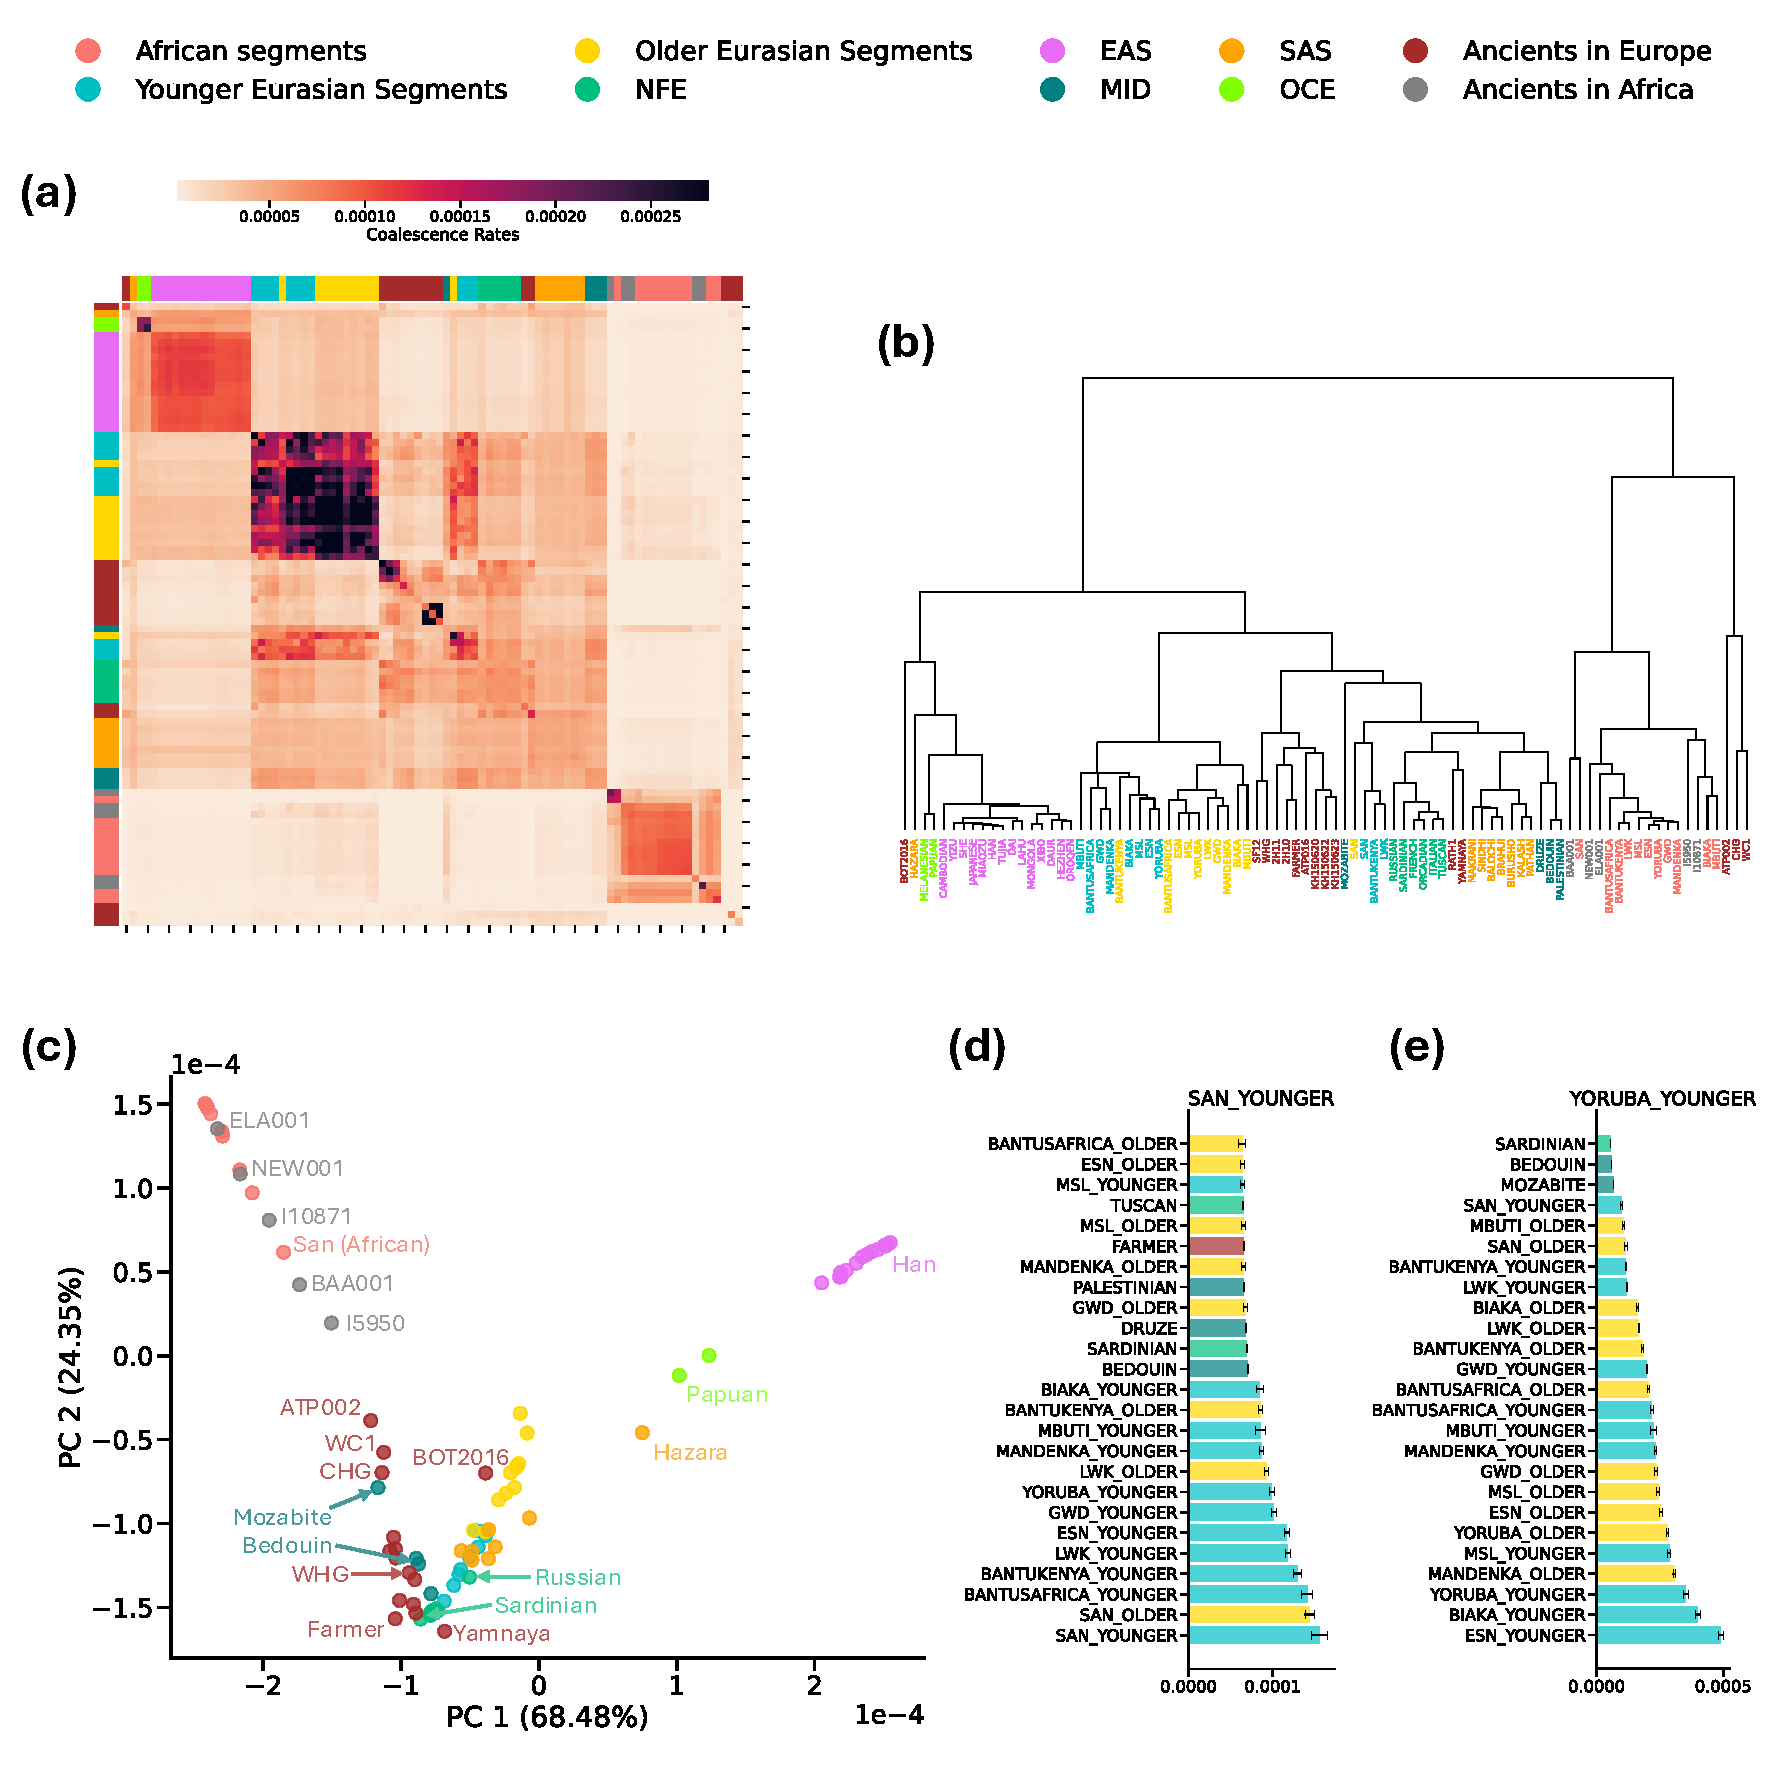
\includegraphics[width=\linewidth]{figures/gb_bta/gb_real_bta_12.pdf}
    \captionsetup{width=\textwidth+3cm}
    \caption{
    \footnotesize
    \textbf{Coalescence rates with modern and ancient samples.} (a) Matrix of pairwise coalescence rates for all modern and ancient groups in the epoch spanning $10{,}000$–$15{,}848$ years. (b) Dendrogram corresponding to the UPGMA hierarchical clustering of the pairwise coalescence rate matrix in (a). (c) PCA visualization of coalescence rates for the epoch spanning $10{,}000$–$15{,}848$ years, with PC1 and PC2 representing the eigenvectors capturing the greatest variance among modern samples. (d-e) Top $25$ groups based on coalescence rates with (d) younger Eurasian-like segments in the San, and (e) younger Eurasian-like segments in Yoruba during the epoch spanning $10{,}000$–$15{,}848$ years. Row and column colors in (a), dendrogram leaves in (b), and dots and bars in (c-e) are colored according to the common legend. NFE = non-Finnish Europeans, EAS = East Asians, MID = Middle Easterners and North Africans, SAS = South Asians, OCE = Oceanians. The numbers in brackets in (c) indicate the proportion of variance explained by each principal component. The error bars in (d-e) represent 95\% confidence intervals calculated using $100$ bootstraps. Results derived from HGDP+$1{,}000$GP+aDNA+archaic genealogies.
    }
\label{fig:gb-bta-source}
\end{figure}

\clearpage

% In order to characterize the admixture event further
% only focus on recent event
% We use the genealogies with moderns and ancients and calculate coal. rates given our local ancestry
% Do it seperately per population

%% Coal. rate epoch for moderns 0-10kya, for ancients 10kya-20kya
%% insert another figure with map with proportions, dates and source group per population - for younger admixture event only

% \subsection{Signatures of adaptive introgression}

% Admixture introduces new alleles into a population, some of which may be beneficial. This often manifests as an excess of one ancestry type at loci under selection. Using the local ancestry inferred with GhostBuster, we derive a selection statistic to measure the excess of Eurasian ancestry within African genomes, focusing specifically on ancestry from the younger admixture event. We define the selection statistic at each site based on the average Eurasian ancestry across all African samples in the HGDP+$1{,}000$GP dataset. To model this, we fit a beta-binomial distribution to the average Eurasian ancestry across sites, allowing for genetic drift, which can cause ancestry proportions to vary along the genome. Finally, we calculate p-values for excess Eurasian ancestry at each site based on the fitted beta-binomial distribution.

% We analyzed $270{,}000$ locations along the genome, excluding regions within or 50 kb around ENCODE blacklist regions \cite{amemiya2019encode}. The ENCODE blacklist identifies problematic genomic regions prone to artifacts in high-throughput sequencing, often due to excessive repeats, satellite sequences, or other anomalies that can interfere with accurate analysis. 

\section{Evidence of a deep admixture event in Africans}
\label{sec:ch3-gb-deep}

% The existence of deep population structure in Africa has ignited considerable debate in recent years, with multiple theories proposed to explain this complex evolutionary history. One hypothesis suggests the presence of ghost populations -- especially in regions of West Africa \cite{durvasula2020recovering}. Another theory, known as the “weakly structured stem” model, proposes the existence of multiple ancient populations more than $100{,}000$ years ago, which subsequently merged in varying proportions to form present-day African populations \cite{ragsdale2023weakly}. A third perspective highlights the role of gradual, continuous migration across populations, suggesting that African populations became blends of diverse ancestral groups \cite{lipson2020ancient}.

We used GhostBuster to understand the deep evolutionary history in Africa. Our analysis incorporates the same set of modern and ancient African samples as used in the ``Back-to-Africa'' section, detailed in Table \ref{tab:african_populations}. 

\subsection{Ancient admixture across sub-Saharan African populations}

To examine ancient events, we focused on coalescence events that occurred between $10{,}000$ and $5{,}000{,}000$ years ago, dividing this time frame into 20 epochs on a logarithmic scale. We excluded coalescence events more recent than $10{,}000$ years, as these likely represent more recent events like previously discussed back-to-Africa migrations. Consistent with previous analyses of back-to-Africa migration, we grouped non-Finnish Europeans (NFE), East Asians (EAS), and South Asians (SAS) as Eurasians. For each African population, analyses were conducted using all Eurasian and African populations in the dataset as reference groups, while excluding Middle Eastern and American populations from the reference panel. To further concentrate on broader lineage relationships, coalescence events between individuals within the target population were excluded. 
%To control for confounding effects due to back-to-Africa migration, we masked both the younger and older back-to-Africa segments, as identified in section \ref{sec:ch3-gb-bta}, from the local ancestry estimates.

Starting from a random initialization, the coalescence rates converged to reveal two distinct components. Figure \ref{fig:gb_deepadmix_1}a shows the inferred coalescence rates in Yorubans, used as a representative group. These rates suggest two components that primarily differ in their coalescence rates with Eurasians. We refer to the component closer to Eurasian populations as the out-of-Africa-like (OOA-like) component and the one relatively closer to African populations as the non-out-of-Africa-like (non-OOA-like) component. The Eurasian-like ancestry previously identified in Section \ref{sec:ch3-gb-bta} strongly correlates with the OOA-like component in this deep admixture, with more than $98$\% of segments attributed Eurasian-like lying within this component. This correlation is largely explained by the component's faster coalescence rate with Eurasians and supports the presence of two distinct types of Eurasian ancestries in Africans, as discussed in Section \ref{sec:ch3-gb-bta}. To specifically examine this deeper admixture events, we masked regions corresponding to previously identified Eurasian-like segments (posterior probability Eurasian-like > 10\%) and a $100$kb flanking region around them to avoid biases from recent back-to-Africa migration.

Both the held-out likelihood and the expected coefficient of determination indicate that two components best capture the observed coalescence differences without ambiguity regarding the admixture event (see Figure \ref{fig:gb_deepadmix_1}b and Figure \ref{fig:gb_deepadmix_cv_all}). We identified varying proportions of OOA-like and non-OOA-like components across modern and ancient African groups after removing ancestry corresponding to the back-to-Africa migration. Among modern groups in the HGDP+$1{,}000$GP and SGDP datasets, Dinka individuals exhibited the highest proportion of OOA-like ancestry at approximately $36.8$\%, while Khomani San individuals showed the lowest at $10.6$\%. In ancient individuals, we detected $35.9\%$ OOA-like ancestry in the $4{,}500$-year-old Mota individual, $27.6\%$ in a $7{,}900$-year-old ancient African from Cameroon, and $30.1\%$ in younger ancient samples from South Africa, namely ela001 and new001. In contrast, the Ballito Bay individual, baa001, exhibited $12.3\%$ OOA-like ancestry. Overall, we observed a higher proportion of the OOA-like component in East Africa, followed by West and South Africa, with the lowest levels in Central African hunter-gatherers (see Figure \ref{fig:gb_deepadmix_1}d). The first four principal components of the coalescence count and opportunity matrix did not reveal substantial differences between clusters (see Figure \ref{fig:gb_deepadmix_1}b). This is attributable to the large number of African reference panel groups compared to a single group representing Eurasians, which exhibit less variation between the components inferred by GhostBuster.

\begin{figure}[h!]
    \centering
    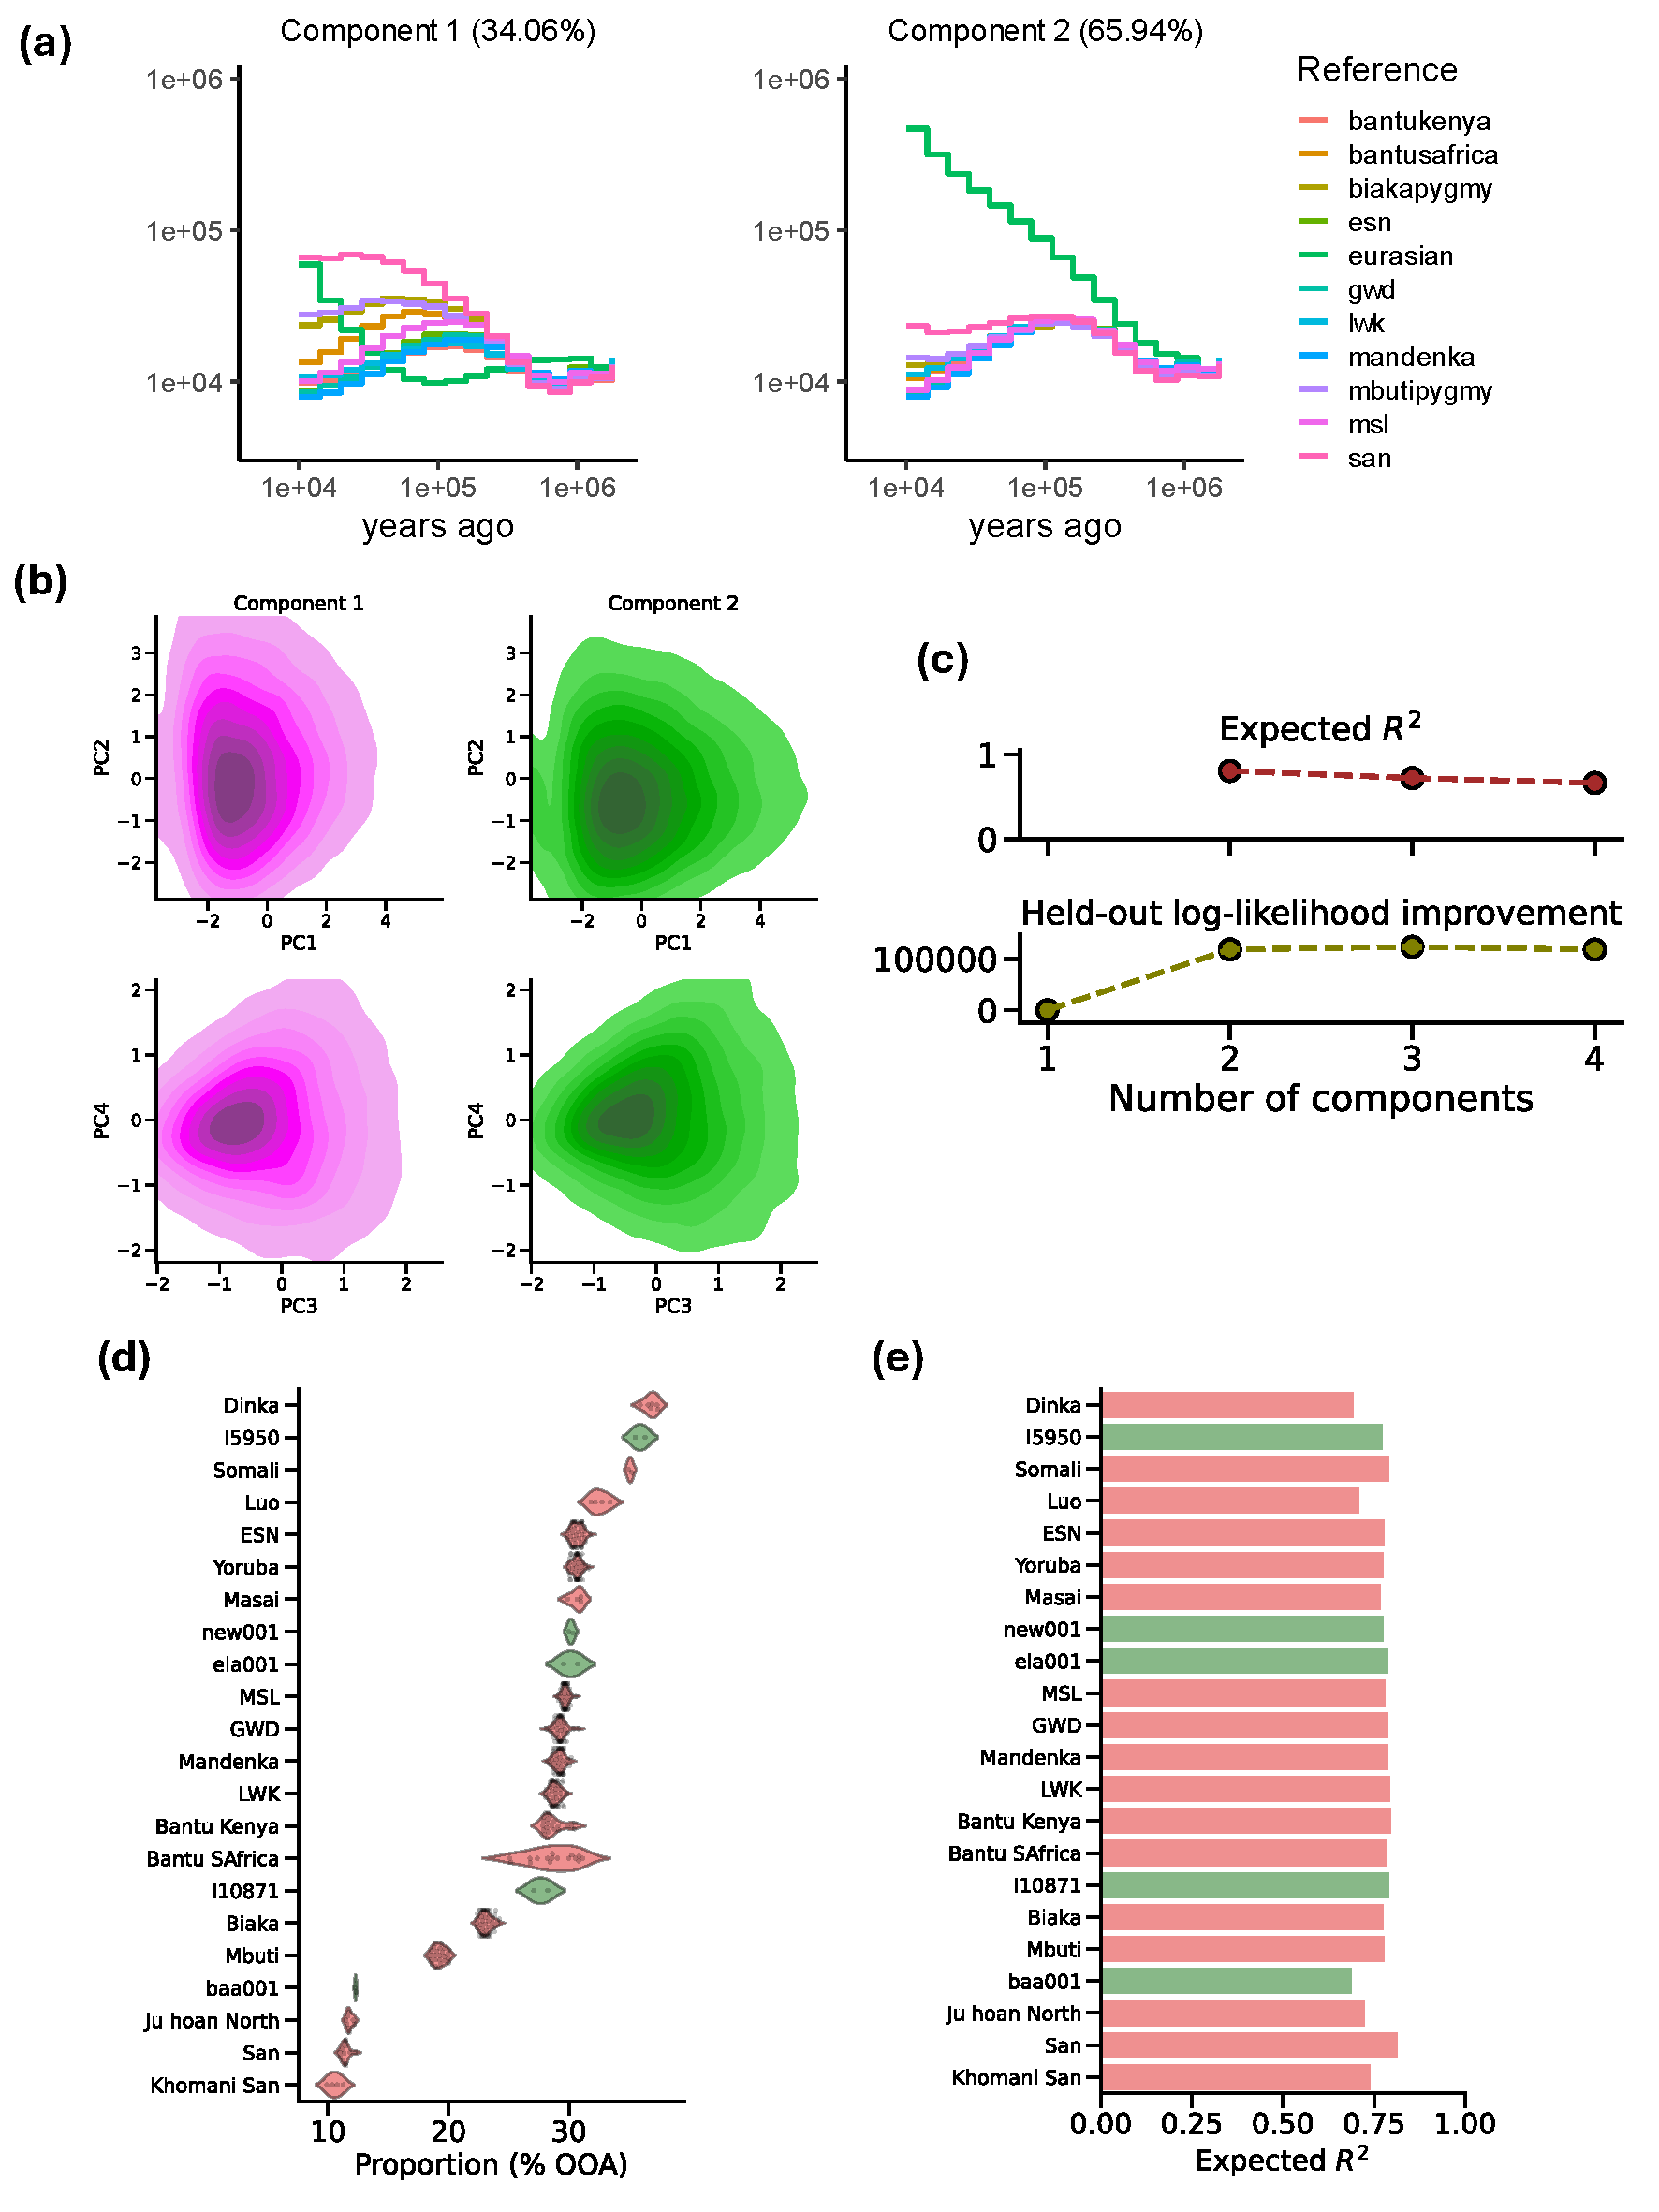
\includegraphics[width=\linewidth]{figures/gb_deepadmix/gb_real_deep_1.pdf}
    \captionsetup{width=\textwidth+3cm}
    \caption{
    \footnotesize
    \textbf{Decomposing sub-Saharan Africans to find a deep admixture event.} (a) Inferred inverse coalescence rates and proportions when decomposing Yorubans: each line represents inverse coalescence rate profiles with a reference population. (b) PCA visualization of the coalescence count and opportunity matrix derived from the genealogies plotted separately for each component. (c) Expected coefficient of determination and held-out log-likelihood improvement with varying number of components. (d) Proportion of the out of Africa-like ancestry and (e) Expected coefficient of determination across all African populations analyzed. The PCA visualization in (b) is based on a KDE plot with a threshold of 0.05, and binary local ancestry estimates are obtained by thresholding the inferred posteriors at 0.5. Individual data-points overlaid on the violin plots. 
    }
    \label{fig:gb_deepadmix_1}
\end{figure}

\clearpage

\subsection{Dating the admixture event}

We constructed coancestry curves using the inferred local ancestry data without filtering out previously identified back-to-Africa segments. These curves were then used to fit various admixture dating models, including single-date, two-date, and continuous admixture models. Similar to the back-to-Africa migration, we found that a single-date model did not provide a good fit to the coancestry curves. Notably, the two-date admixture model provided the best fit for the coancestry data across 10 out of 16 African populations (see Figure \ref{fig:gb_deepadmix_3}). Consistent with the back-to-Africa migration, the younger admixture dates ranged from $1{,}500$ to $7{,}000$ years ago, while the older admixture event occurred approximately $23{,}000$ to $40{,}000$ years ago (see Figure \ref{fig:gb_deepadmix_3}).

Next, we removed the local ancestry in and around the Eurasian-like segments previously identified in Section \ref{sec:ch3-gb-bta} and recalculated the coancestry curves. After removing the local ancestry corresponding to the more recent back-to-Africa migration, we found that the single-date admixture model fit the coancestry data as well as the two-date and continuous admixture models in most scenarios (see Figure \ref{fig:gb_real_deep_dating_wobta}). This suggests that the younger date in the initial fit most likely captures the more recent back-to-Africa migration. Therefore, we focus on the older date as the estimated time of admixture between OOA-like and non-OOA-like populations and exclude the Eurasian-like ancestry identified in the back-to-Africa section from all subsequent analyses. This admixture is dated to  $23{,}000$-$40{,}000$ years across groups (see Table \ref{tab:gb_deep_admix_dates}). It is important to note that these admixture dates have not been adjusted for potential errors in the recombination map, as we lacked reliable error estimates for it. We believe this may introduce a downward bias in the dating estimates \cite{sankararaman2012date}. However, it might be reasonable to assume that the admixture occurred around or after the out-of-Africa migration dated around $50{,}000$–$100{,}000$ years ago \cite{lopez2015human}. 

Given the deep nature of the admixture, we performed additional ``sanity checks'', such as running GhostBuster with the HMM disabled and using only African reference populations (removing Eurasians). These analyses produced similar coalescence rates and correlated but more uncertain local ancestry estimates compared to the initial run with the HMM enabled and Eurasian samples included in the reference population (see Figure \ref{fig:gb_deepadmix_sanity1} and \ref{fig:gb_deepadmix_sanity2}).

\begin{figure}[h!]
    \centering
    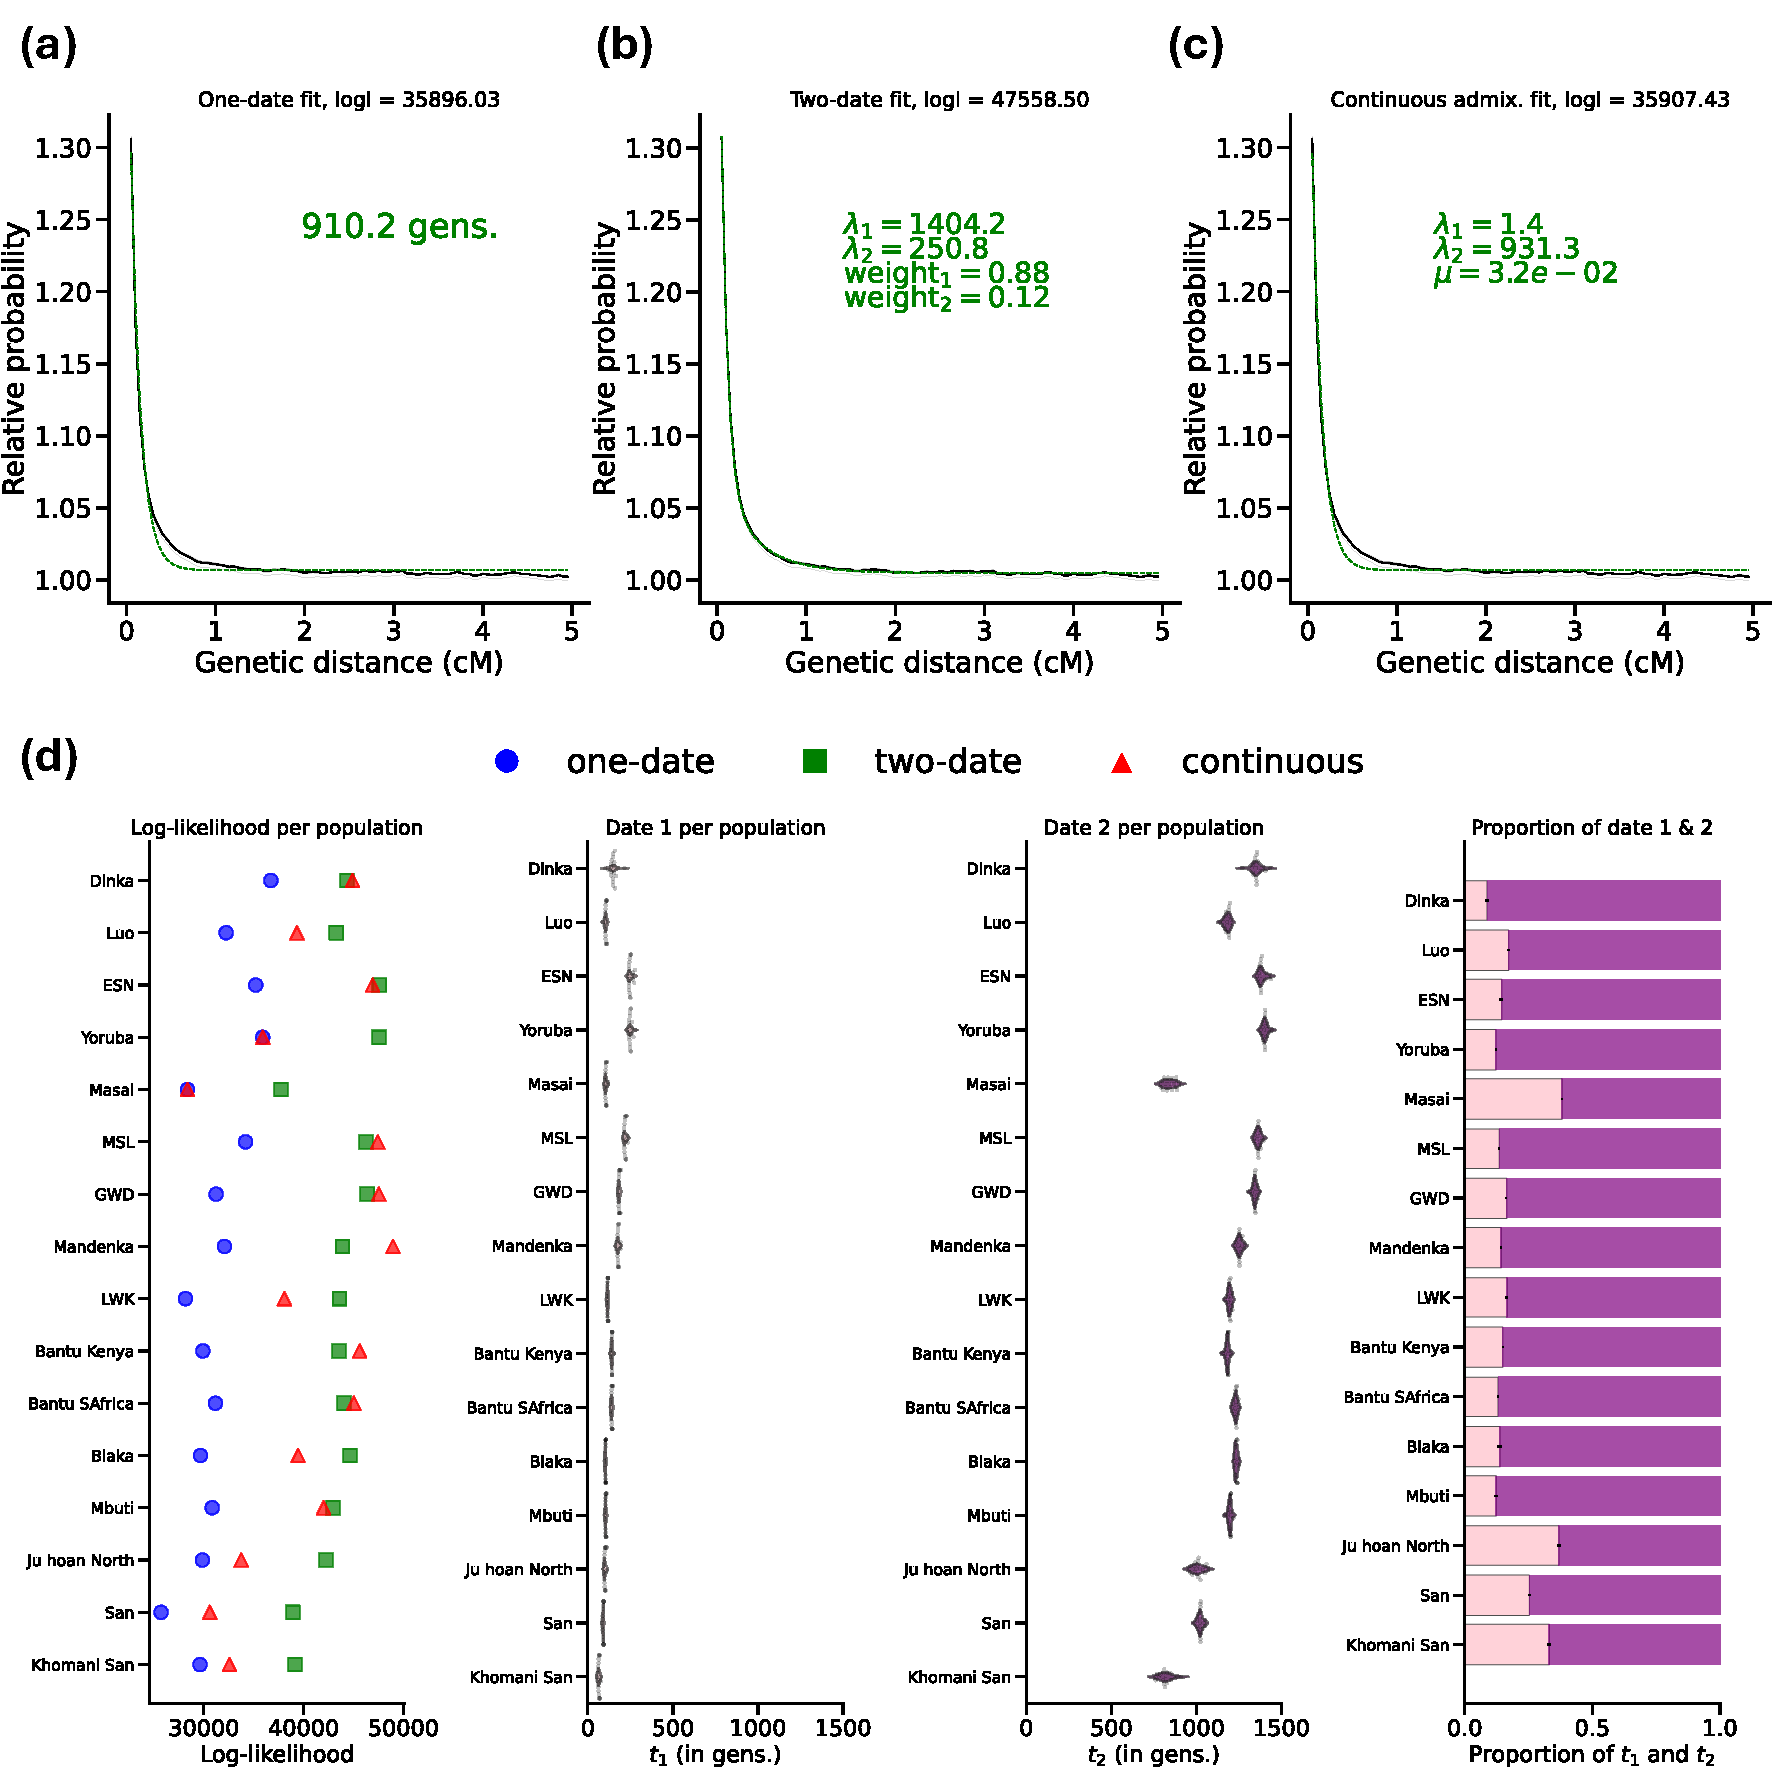
\includegraphics[width=\linewidth]{figures/gb_deepadmix/gb_real_deep_3.pdf}
    \captionsetup{width=\textwidth+3cm}
    \caption{
    \footnotesize
    \textbf{Dating the ancestral components corresponding to deep admixture event.} Coancestry curves and (a) one-date admixture model fit, (b) two-date admixture model fit and (c) constant migration rate continuous admixture model fit for Yorubans. (d) Per-population least squared log-likelihood corresponding to various admixture models along with the admixture dates and weights inferred using two-date admixture model. The log-likelihood values are aggregated across $20$ jackknife runs. Populations are sorted based on highest to lowest proportion of Eurasian-like ancestry, pink represents the younger admixture date and purple represents the older admixture date in (d). Individual data-points overlaid on the violin plots. Admixture dates in the plot are in generations.
    }
    \label{fig:gb_deepadmix_3}
\end{figure}

\clearpage

\subsection{Mutational profiles validate the admixture event}
\label{sec:ch3-gb-deep-mut}

We used mutation profiles as near orthogonal evidence that GhostBuster has identified two distinct components that are unlikely to be data or method artefacts. Similar to the analysis in Section \ref{sec:ch3-gb-bta-mutational}, we calculated the normalized mutational enrichment profiles for continental populations and inferred mixture components relative to genome-wide normalized mutation rates in the African population.

In contrast to our analysis of the more recent back-to-Africa migration, we did not observe enrichment for TCC to TTC mutations (see Figure~\ref{fig:gb-mutational-all-deep}). This is likely because this admixture event predates the emergence of TCC to TTC mutations in Eurasian populations. However, we detected distinct patterns in the enrichment of weak to strong mutations between the two ancestry components. To classify mutations as weak or strong, CpG sites were excluded, following the approach used in analyzing the back-to-Africa migration. We observed a reduction of weak to strong mutations in the out-of-Africa-like (OOA-like) component compared to genome-wide weak to strong mutation rates within Africa. This reduction peaked approximately $50{,}000$ -- $100{,}000$ years ago, aligning with patterns observed in other Eurasian populations (see Figure \ref{fig:gb-mut-ws-deep}a-b). These findings suggest a notable divergence in the trajectories of existing mutations during this period, driven by differential GC-biased gene conversion between the two ancestral components. Among ancient samples, the $4{,}500$-year-old individual from Mota Cave (I5950) and the $400$-year-old individual from South Africa (new001) exhibited approximately double the weak-to-strong mutation reduction signal compared to modern samples (see Figure \ref{fig:gb-mut-ws-deep}c). This increase cannot be attributed to our estimated uncertainty and may suggest that the OOA-like group ancestors for these individuals experienced a particularly small effective population size. In contrast, the $1{,}900$- and $500$-year-old individuals from South Africa (baa001 and ela001) displayed a subtle weak-to-strong signal reduction in the OOA-like group, similar to what is observed in modern-day samples (see Figure \ref{fig:gb-mut-ws-deep}c). Meanwhile, the $7{,}900$-year-old individual from Cameroon (I10871) showed no significant difference in weak-to-strong enrichment between the two components (see Figure \ref{fig:gb-mut-ws-deep}c).

\begin{figure}
    \centering
    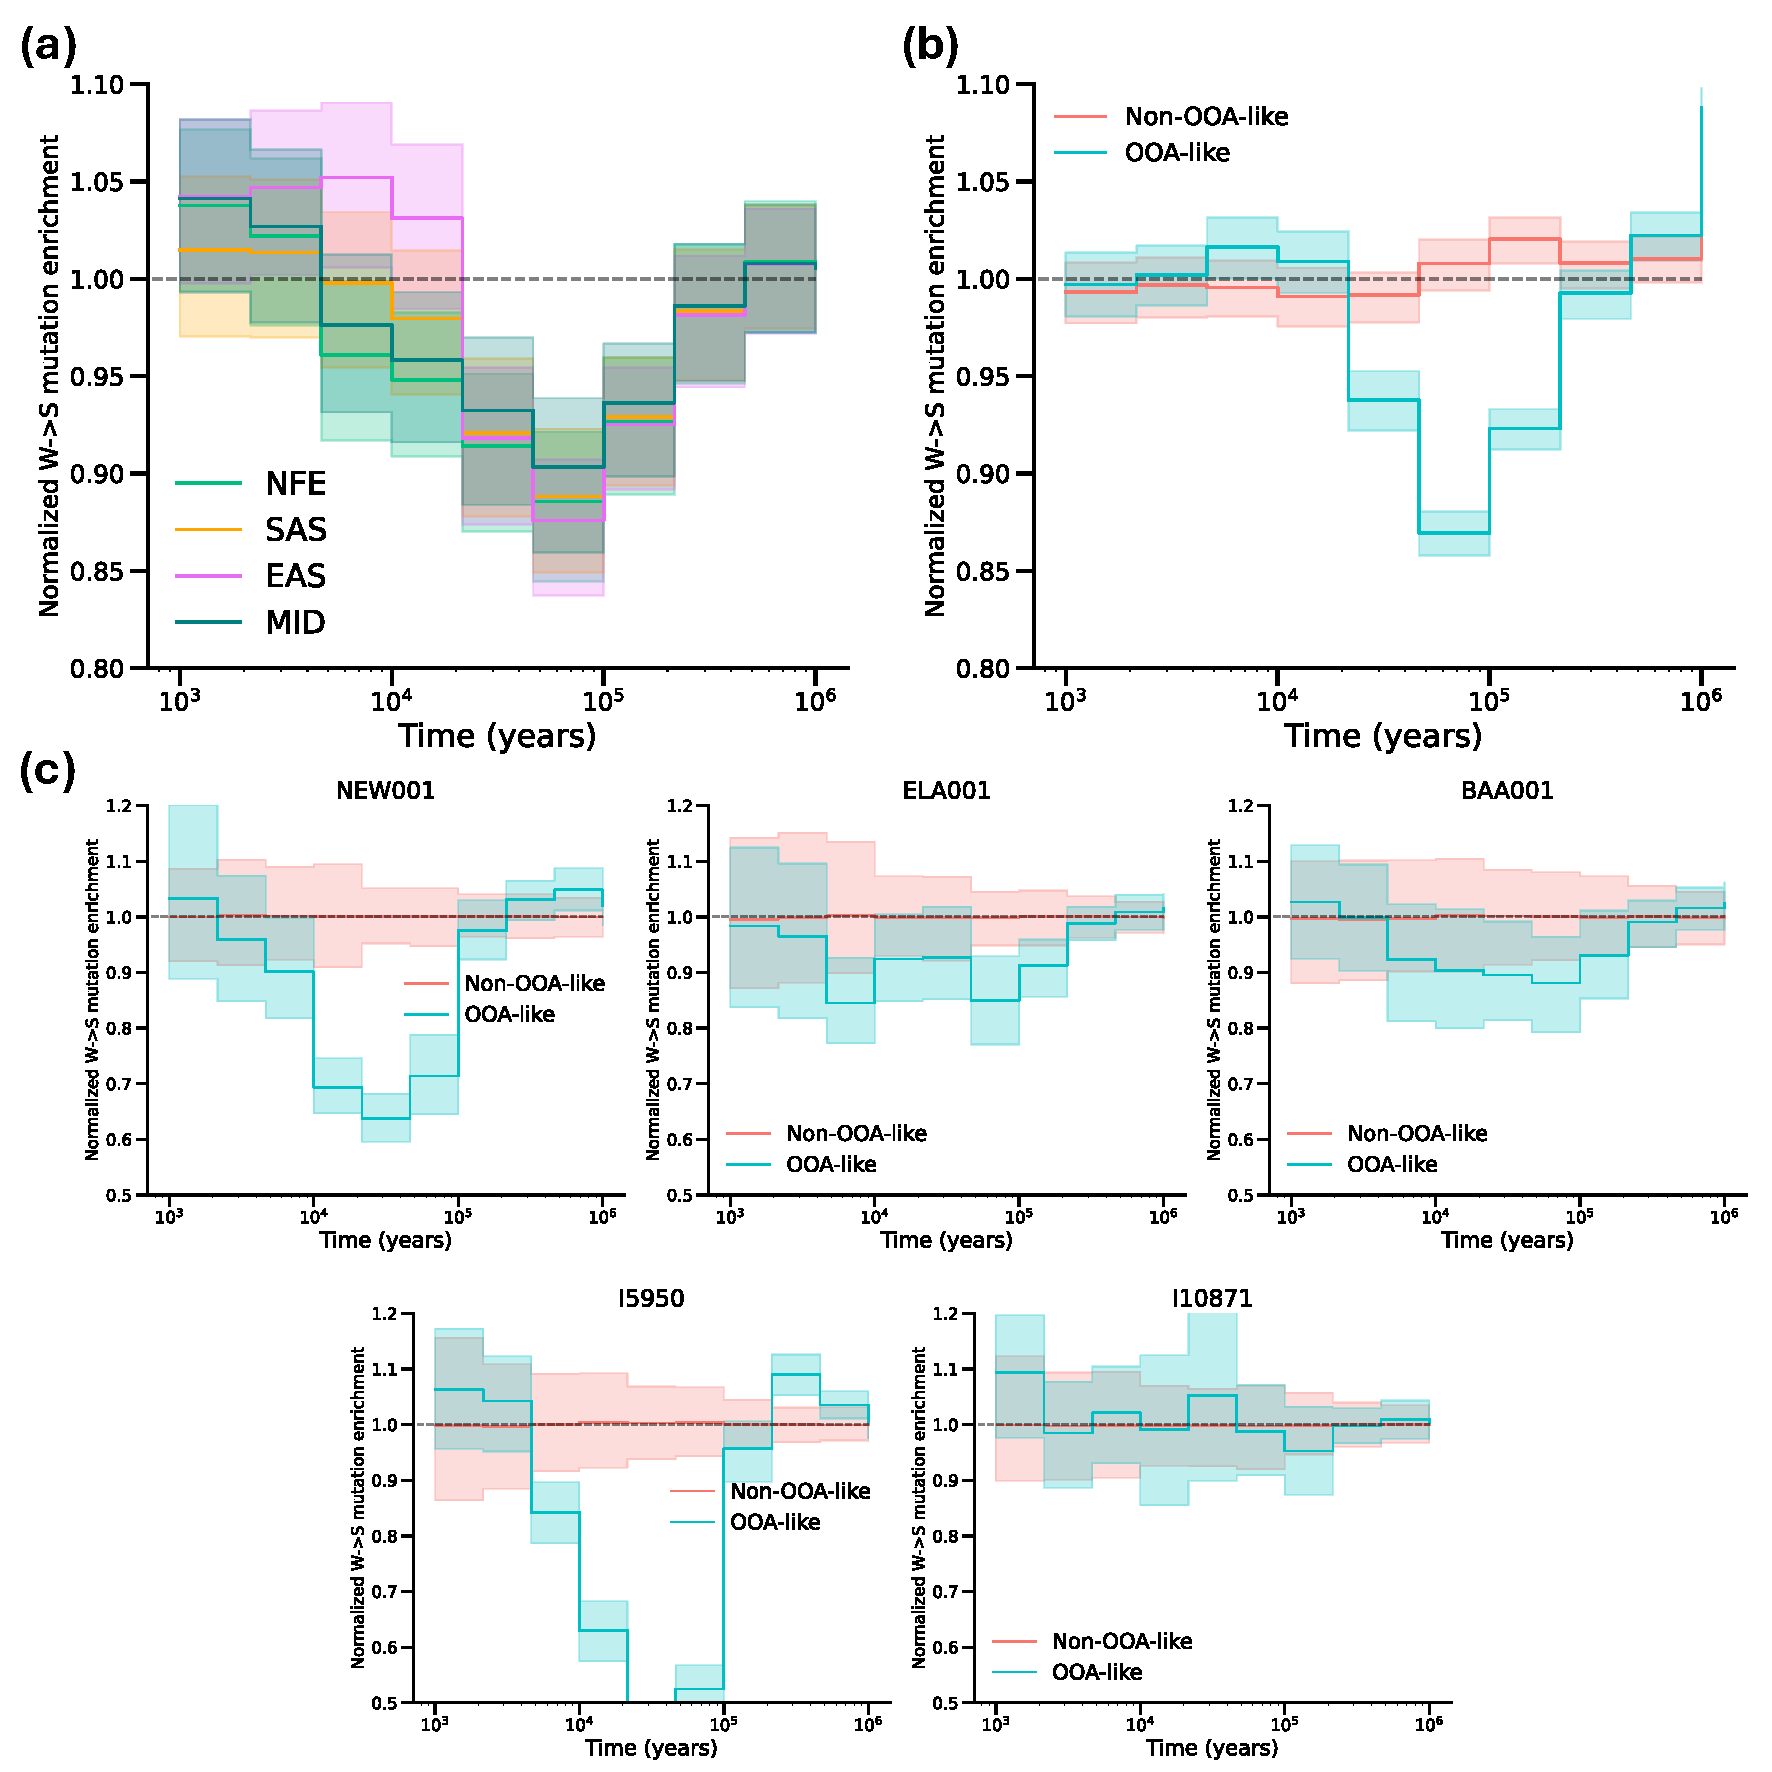
\includegraphics[width=\linewidth]{figures/gb_deepadmix/gb_real_deep_8.pdf}
    \captionsetup{width=\textwidth+3cm}
    \caption{
    \footnotesize
    \textbf{Enrichment of weak to strong mutation rates in the deep admixture African components.} (a) Enrichment of weak to strong mutation rates across various continental groups, including NFE (non-Finnish Europeans), SAS (South Asians), EAS (East Asians), and MID (Middle Eastern and North African populations). (b) Enrichment of weak to strong mutation rates in OOA-like and non-OOA-like (African) segments in African populations. (c) Weak to strong mutation rate enrichment in five ancient African samples, including new001, ela001, baa001, I5950, and I10871 (see population descriptions in Table \ref{tab:african_populations_2}). Shaded regions indicate 95\% confidence intervals derived from $1{,}000$ bootstrap replicates, while the dashed line represents the baseline of no enrichment. Results derived from HGDP+$1{,}000$GP and HGDP+$1{,}000$GP+aDNA+archaic genealogies.
    }
\label{fig:gb-mut-ws-deep}
\end{figure}

\clearpage

\subsection{Variation in PRDM9 activity across populations}
In humans, recombination predominantly occurs at specific regions in the genome known as recombination hotspots. The placement of these hotspots is largely governed by the PRDM9 gene, which encodes a zinc finger protein responsible for identifying and binding to distinct DNA sequence motifs. Once bound, PRDM9 modifies histones near the binding sites, creating an environment conducive to recombination initiation.

Multiple types of PRDM9 have been identified in humans, distinguished by variations in the zinc finger array configuration. These PRDM9 types can bind to different sequence motifs across the genome, resulting in distinct recombination hotspot locations. Of all the known PRDM9 types in humans, PRDM9-A is the most common, binding to a specific sequence motif (``CCNCCNTNNCCNC'') \cite{coop2008high,myers2008common}. It is present in all modern human populations but absent in chimpanzees \cite{myers2010drive}. PRDM9-B shares most of its binding motif with PRDM9-A and thus targets similar hotspot locations. Another notable PRDM9 type, PRDM9-C, binds to a distinct sequence motif, a unique 17-base pair sequence (``CCgCNgtNNNCgtNNCC''), which directs recombination events to different genomic locations. The small letters in the motif indicate less conserved bases. PRDM9-C is particularly common in African populations but occurs less frequently in Eurasian populations \cite{hinch2011landscape,wegmann2011recombination,alleva2021cataloging}. Importantly, the probability of crossover hotspots associated with PRDM9-C is strongly influenced by the alleles an individual carries at the PRDM9 gene (rs6889665, $p<10^{-245}$ \cite{hinch2011landscape}). 

The recombination machinery repairs double-strand breaks with a slight preference for incorporating GC alleles over AT alleles, leading to GC-biased gene conversion and an increased rate of weak to strong mutations around recombination hotspots. Separately, frequent DNA repair at these hotspots gradually erodes the sequence motifs that PRDM9 zinc fingers bind to, a phenomenon known as hotspot death. The continual loss of hotspots places evolutionary pressure on PRDM9 to form new hotspots through alterations in its zinc finger domains, changing its binding specificity. Consequently, PRDM9 has become one of the fastest-evolving genes, constantly adapting to balance hotspot erosion and renewal \cite{myers2010drive,baker2017repeated}. While the locations of recombination hotspots are determined by the specific PRDM9 allele an individual carries, examining GC-biased gene conversion and signatures of hotspot death at these sites provides insight into the evolutionary history of a lineage. We leverage this evolutionary information to improve our understanding and provide independent evidence of the ancient admixture event under investigation.

We begin by examining the PRDM9-C allele (rs6889665), which has previously been shown to strongly predict the probability of crossover at PRDM9-C hotspots \cite{hinch2011landscape}. In our dataset, we found the SNP rs6889665 to have a frequency of $33.7\%$ in Africans, $8.4\%$ in East Asians, $7.4\%$ in South Asians, and $6.3\%$ in non-Finnish Europeans. Additionally, its frequency was $44.1\%$ in the non-out-of-Africa (non-OOA-like) component but only $2.7\%$ in the out-of-Africa-like (OOA-like) component. Figure \ref{fig:gb_deep_prdm9c_tree} depicts the tree at PRDM9, identifying rs6889665 as one of the oldest mutations on the tree. Notably, the mutation shows an excess of descendants inferred to possess ancestry from the non-OOA-like component compared to the OOA-like component.

Next, we analyzed the PRDM9-A and PRDM9-C hotspots along the genome (provided by Dr. Anjali Hinch) to investigate differences in their evolutionary histories across various populations and ancestral components involved in the deep admixture event. Specifically, we examined weak to strong mutations in and around these hotspots and their impact on different populations. PRDM9-A and PRDM9-C hotspots were analyzed separately, excluding regions where both hotspots occur within a 5kb interval. Consistent with the mutational enrichment analysis, CpG sites were excluded when classifying mutations as weak or strong. 

To understand population-level differences in PRDM9 activity, we began by examining the number of descendants carrying the weak to strong mutations at these hotspots per population. This quantity was normalized by the total number of population samples in the dataset and the AT content of the region. Furthermore, we only considered mutations with an age of less than one million years. Figure \ref{fig:gb_deepadmix_prdm9_hotspot}a,c presents the normalized descendant count per continental population as a function of the distance from the hotspot center for weak to strong mutations. For hotspots associated with PRDM9-A, we observed similar peak intensities around the hotspot center across all continental populations analyzed. In contrast, PRDM9-C hotspots exhibited differences in activity across continental populations, with Africans showing a higher peak compared to non-African populations. This discrepancy could be attributable to population-specificity of PRDM9-C allele previously identified \cite{hinch2011landscape, alleva2021cataloging}.

To explore differences in weak to strong mutation rates across the ancestral components involved in the deep admixture event, we analyzed weak to strong mutations within $1{,}000$ bp of the hotspot center and calculated the time-stratified mutation rate enrichment as described in Section \ref{sec:ch3-gb-deep-mut}. However, it is important to note that while Relate provides estimates of mutational ages, its accuracy within hotspots is limited. These estimates are likely correlated with true ages, but they should not be interpreted as highly precise chronological markers. Unlike the genome-wide mutational enrichment analysis, we normalized the enrichment relative to the mutation rate in East Asians (rather than Africans) and focused exclusively on regions around the hotspots. 

Figure \ref{fig:gb_deepadmix_prdm9_hotspot}b,d illustrates the weak to strong mutation rate enrichment for the OOA-like and non-OOA-like components at PRDM9-A and PRDM-C hotspots respectively. Relative to the weak to strong mutation rate in East Asians, both the OOA-like and non-OOA-like components exhibited enrichment for weak to strong mutations around $50{,}000$ years ago at PRDM9-A hotspots. 
%
This enrichment was of a similar magnitude for both components. However, in regions near PRDM9-C hotspots, we observed a significant difference in enrichment between the two components (see Figure \ref{fig:gb_deepadmix_prdm9_hotspot}d), with the non-OOA-like component exhibiting higher weak to strong mutations. This suggests that the PRDM9-C allele historically exhibited greater activity relative to the PRDM9-A allele in the non-OOA-like group compared to the OOA-like group.
%
This finding, along with the broader differences in GC-biased gene conversion (GCbGC), provides compelling evidence that the two groups represent genuine, ancient population stratification within African ancestral groups. It is difficult to conceive of confounding factors that could misclassify ancestry in a way that would result in distinct mutation types appearing on separate lineages. This is particularly true given that information about mutation type is invisible to GhostBuster and that our normalization procedure for identifying mutational biases explicitly matches the genomic regions used to define OOA-like and non-OOA-like mutation profiles.
%
Furthermore, these patterns align precisely with a priori expectations of ancient stratification. The present-day frequency of PRDM9-C is lower than PRDM9-A in both non-African and inferred OOA-like African individuals, while it is comparatively higher in non-OOA-like African lineages. These observations strongly support the hypothesis of deep population structure within African ancestral groups.
% This enrichment was of a similar magnitude for both components. However, in regions around PRDM9-C hotspots, we observed differential enrichment between the two components, with the non-OOA-like component showing higher weak to strong mutation rates. This suggests that the PRDM9-C allele may have originated in the non-OOA-like population and was subsequently introduced into the OOA-like population through some sort of gene-flow. More importantly, the differential signals at PRDM9-C hotspots provide independent evidence that the structure we are identifying in Africa is likely real. 
Finally, it is worth noting that the mutation rate enrichments shown in Figure \ref{fig:gb_deepadmix_prdm9_hotspot}b,d are based on mutations mapped to the genealogy. A small fraction of mutations (less than $3$\%) do not map to the genealogy and therefore cannot be dated. Nevertheless, we believe the observed signal is robust and unlikely to be affected by these non-mapping mutations.

\begin{figure}[h!]
    \centering
    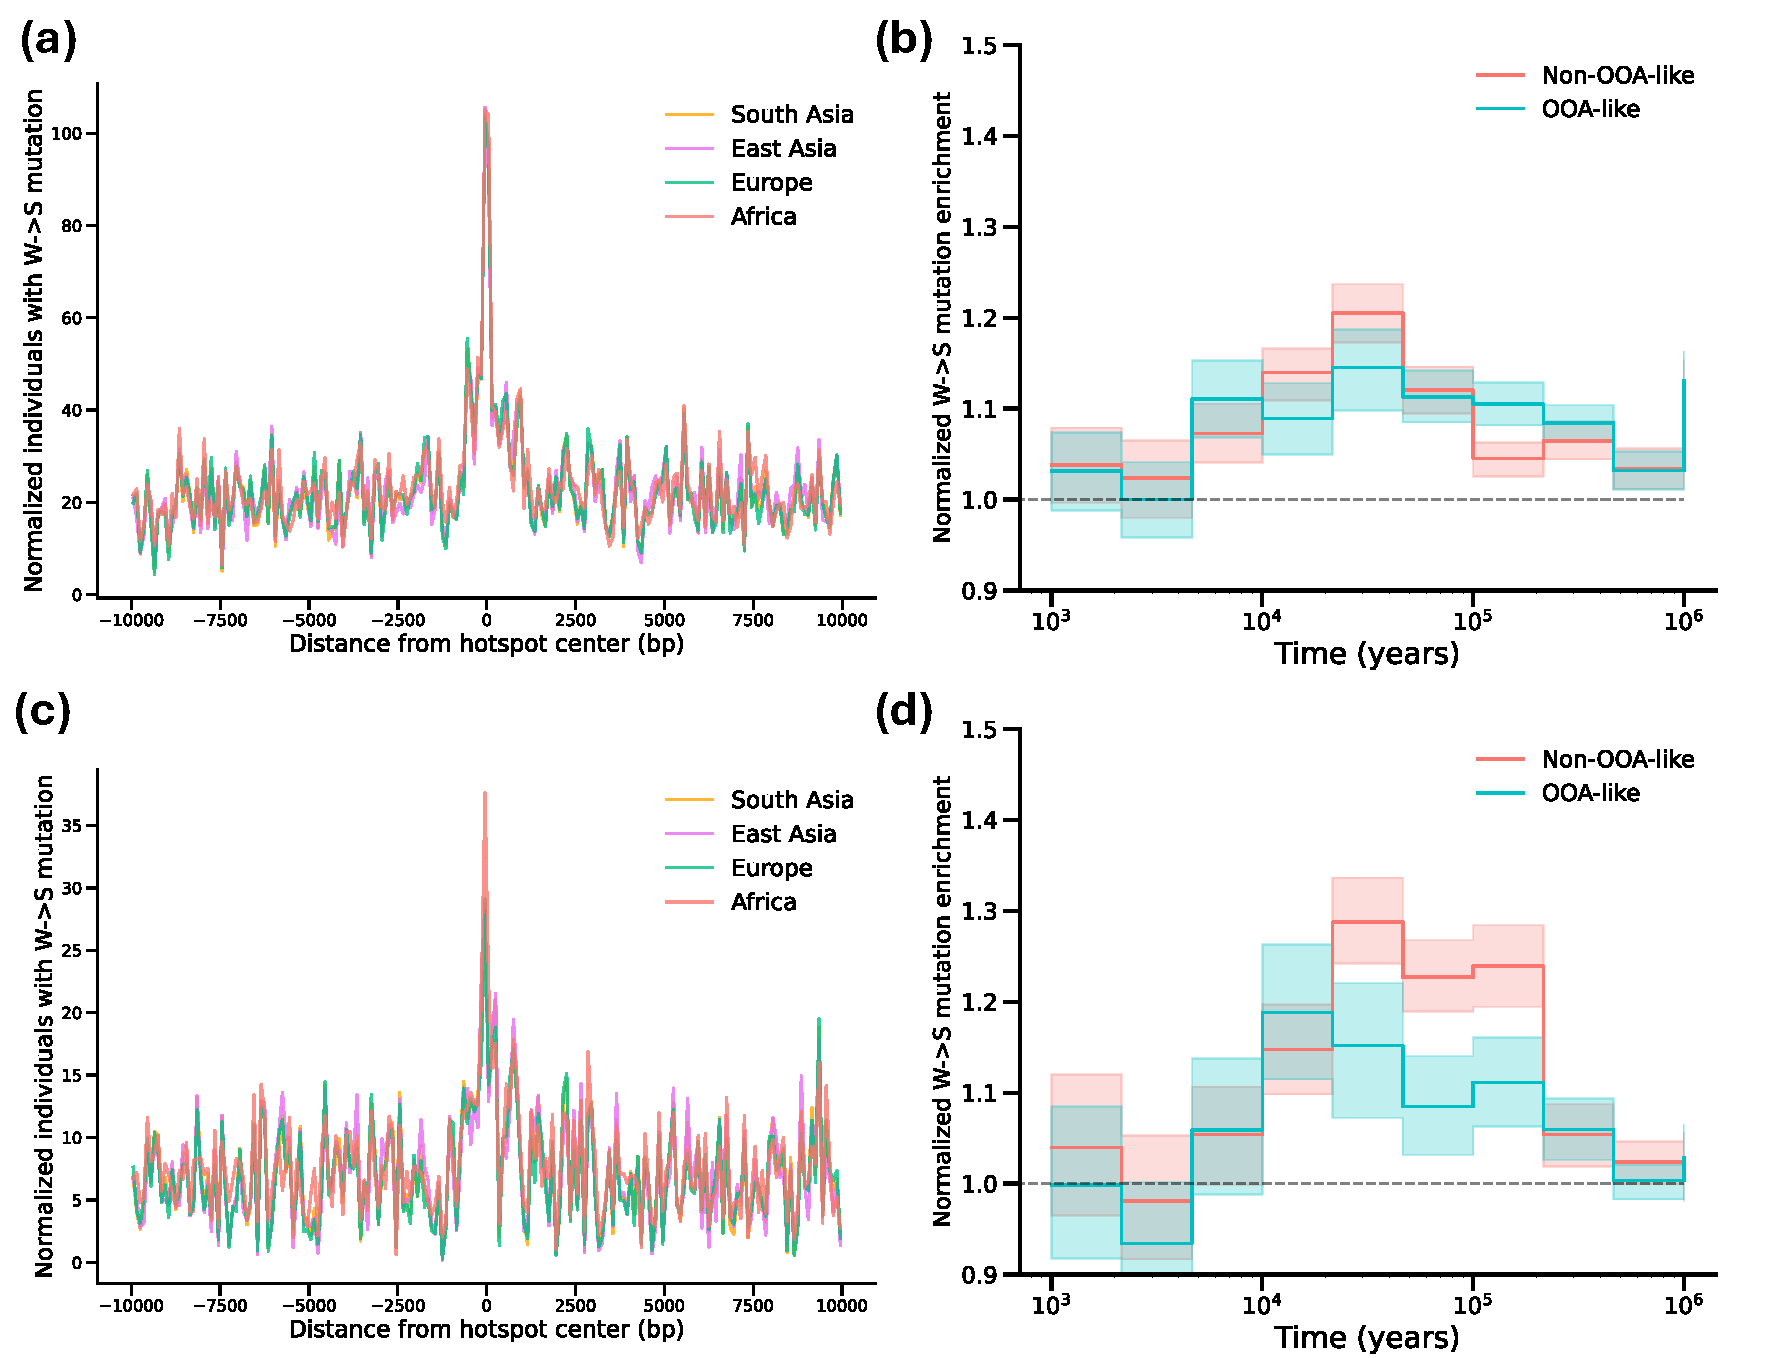
\includegraphics[width=\linewidth]{figures/gb_deepadmix/gb_real_deep_4.pdf}
    \captionsetup{width=\textwidth+3cm}
    \caption{
    \footnotesize
    \textbf{Weak to strong mutation rates at recombination hotspots across populations.} Weak to strong mutation counts across populations and deep admixture component in (a-b) PRDM9-A hotspots, (c-d) PRDM9-C hotspots. Panel (a) and (c) measure the number of individuals carrying weak to strong mutations around the PRDM9 hotspots, normalized by the total number of individuals and the AT content of the region. Whereas, Panel (b) and (d) measure the time-stratified normalized mutation rate enrichment with respect to weak to strong mutation rates in East Asians. In panel (b) and (d) the shaded regions indicate 95\% confidence intervals derived from $1{,}000$ bootstrap replicates, while the dashed line represents the baseline of no enrichment. Results derived from HGDP+$1{,}000$GP and HGDP+$1{,}000$GP+aDNA+archaic genealogies.
    }
    \label{fig:gb_deepadmix_prdm9_hotspot}
\end{figure}

\clearpage

\subsection{Characterizing the admixture event using coalescence rates}
%% split times 
%% Relation with Nea. and Denisovans
%% Relation with OOA population

In order to characterize the deep admixture event better, we look at the relationship of two ancestral components with various modern, ancient and archaic populations. Similar to analysis in Section \ref{sec:ch3-gb-bta-source} we calculate coalescence rates with modern samples from HGDP+$1{,}000$GP dataset and 49 high-coverage ancients and 4 archaic human groups (see Table \ref{tab:gb_ancient_samples}) conditioned on the inferred local ancestry for each African population. 

We consider coalescence events in epoch corresponding to $64{,}000$-$100{,}000$ years in the coalescent history. Following the analysis of the back-to-Africa migration (Section \ref{sec:ch3-gb-bta-source}), we constructed a pairwise coalescence rate matrix, which is visualized using a heatmap, UPGMA dendrogram, PCA, and coalescence rate bar plots for this epoch (see Figure \ref{fig:gb-deepadmix-source}a-e, respectively). The PCA plots in Figure \ref{fig:gb-deepadmix-source}c were inferred by calculating PCA on the coalescence rate matrix corresponding to modern populations and non-OOA-like segments in Africans. We then projected the ancients, archaic and OOA-like segments onto the plot. We found the populations to cluster based on geography and sampling times with distinct continental ancestries corresponding to East Asians, Europeans and non-OOA-like African segments visible in the heatmap and PCA (see Figure \ref{fig:gb-deepadmix-source}a,c). The OOA-like segments clustered better with Eurasian populations than non-OOA-like African population. On the PCA plot, they lie along the cline connecting non-OOA-like segments with Europe - East Asia cline. In the inverse coalescence rate plots, the Eurasian population aligns more closely with the OOA-like segment and is estimated to have split from them approximately $100{,}000$ years ago.

\begin{figure}
    \centering
    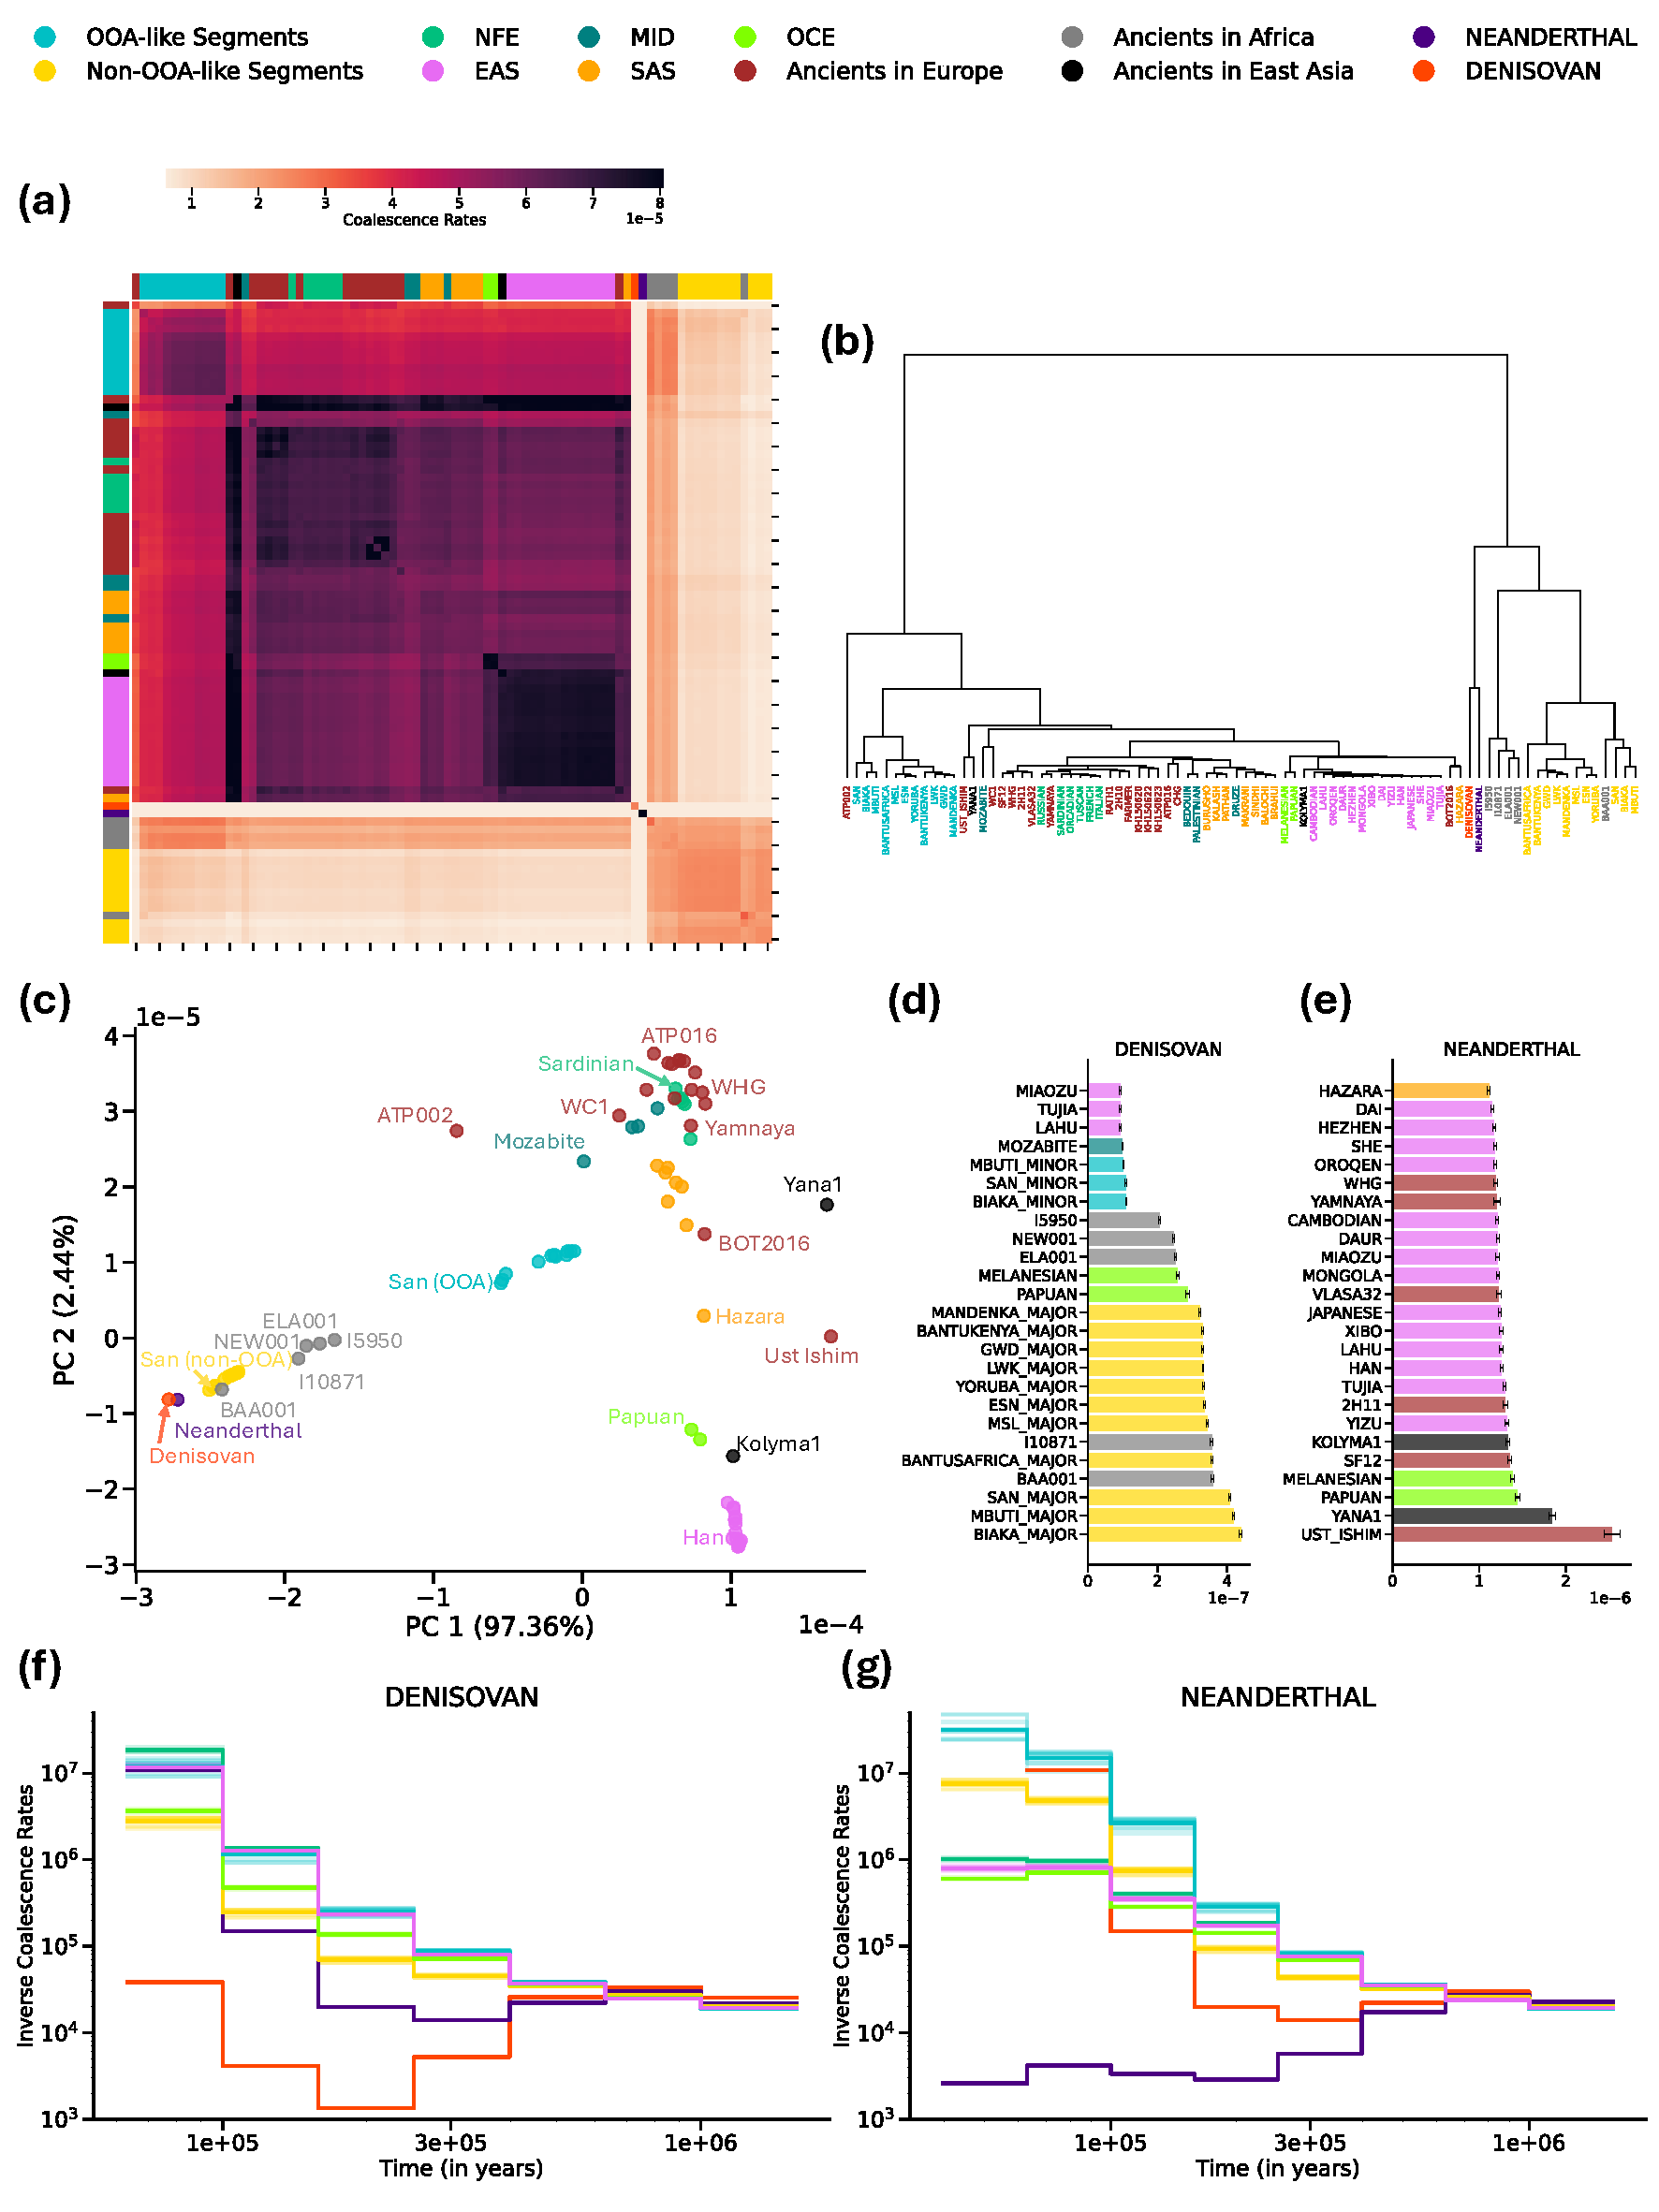
\includegraphics[width=\linewidth]{figures/gb_deepadmix/gb_real_deep_12.pdf}
    \captionsetup{width=\textwidth+3cm}
    \caption{
    \footnotesize
    \textbf{Coalescence rates with modern and ancient samples.} (a) Matrix of pairwise coalescence rates for all modern and ancient groups in the epoch spanning $64{,}000$–$100{,}000$ years. (b) Dendrogram corresponding to the UPGMA hierarchical clustering of the pairwise coalescence rate matrix in (a). (c) PCA visualization of coalescence rates for the epoch spanning $64{,}000$–$100{,}000$ years, with PC1 and PC2 representing the eigenvectors capturing the greatest variance among modern samples. (d-e) Top $25$ groups based on coalescence rates with (d) Denisovan, and (e) Neanderthals during the epoch spanning $64{,}000$–$100{,}000$ years. (f-g) Inverse coalescence rates (ICR) of (f) Denisovan and (g) Neanderthals with other modern human groups from $64{,}000$-$1.6$million years. Darker lines represent population-averaged ICRs.  Row and column colors in (a), dendrogram leaves in (b), dots and bars in (c-e), and lines in (f-g) are colored according to the common legend. NFE = non-Finnish Europeans, EAS = East Asians, MID = Middle Easterners and North Africans, SAS = South Asians, OCE = Oceanians. The numbers in brackets in (c) indicate the proportion of variance explained by each principal component. The error bars in (d-e) represent 95\% confidence intervals calculated using $100$ bootstraps. Results derived from HGDP+$1{,}000$GP+aDNA+archaic genealogies.
    }
\label{fig:gb-deepadmix-source}
\end{figure}

We analyzed coalescence rates in relation to archaic human groups, including three Neanderthal and one Denisovan sample. These samples clustered with the non-OOA-like component (see Figure \ref{fig:gb-deepadmix-source}b). To confirm this observation, we examined coalescence rates across different time epochs and found that both Denisovan and Neanderthal samples consistently exhibited closer relationships to the non-OOA-like component until approximately one million years ago, when all human lineages converge. The coalescence rate patterns suggest ancient migration or admixture events involving these four human groups (see Figure \ref{fig:gb-deepadmix-source}d-g). Furthermore, inverse coalescence rates between Out-of-Africa-like (OOA-like) and non-OOA-like components reveal a deep ancestral split, with the two rates converging at least $300{,}000$ years ago (see Figure \ref{fig:gb_real_deep_coal_ooa}). This predates the divergence of the Eurasian population from the OOA-like component and occurs after the split of Neanderthals and Denisovans from the modern human lineage, although there may be considerable uncertainty in the exact split time.

\begin{figure}
    \centering
    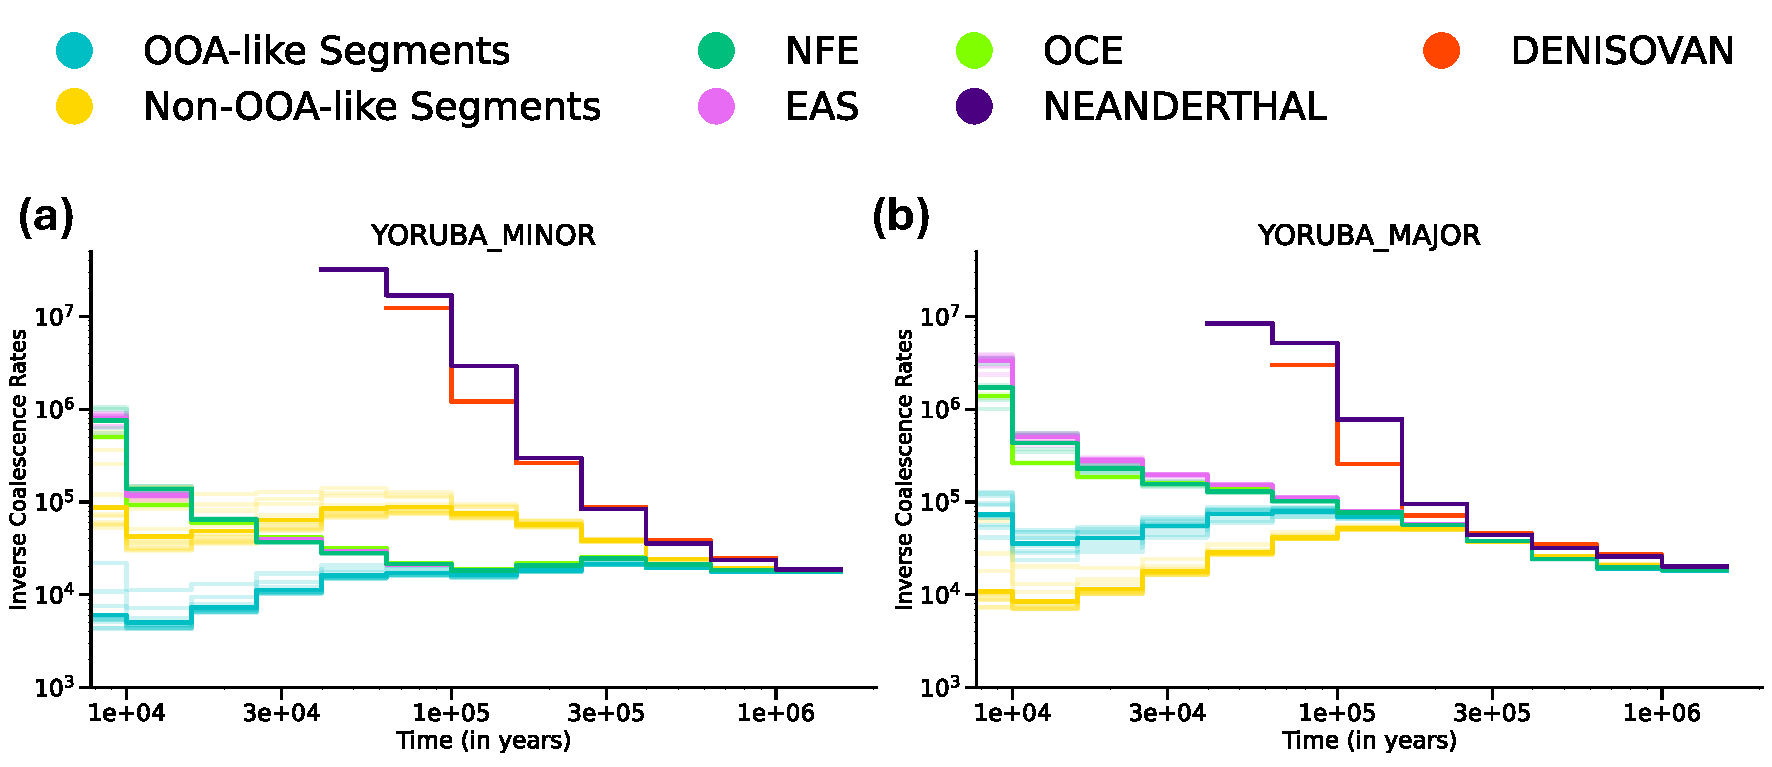
\includegraphics[width=\textwidth]{figures/gb_deepadmix/gb_real_deep_source_coal_rates.pdf}
    \caption{
    \textbf{Inverse coalescence rates (ICRs) of OOA-like and Non-OOA-like component in Yoruba.} ICRs of OOA-like (YOROBA\_MINOR) and Non-OOA-like (YORUBA\_MAJOR) components in Yoruba with other modern human and archaic groups from $64{,}000$-$1.6$million years ago. Darker lines represent population-averaged ICRs and fainter lines represent within population ICRs. NFE = non-Finnish Europeans, EAS = East Asians, MID = Middle Easterners and North Africans, SAS = South Asians, OCE = Oceanians.}
\label{fig:gb_real_deep_coal_ooa}
\end{figure}



\clearpage

\subsection{Impact of the admixture event on polygenic score portability in Africa}

Polygenic scores (PGS) evaluate an individual's genetic predisposition to specific diseases or traits, providing valuable insights into personalized health risks. A PGS is derived from large-scale genome-wide association studies (GWAS), which identify associations between genetic variants and traits of interest. These associations are then used to calculate the risk for a disease or the predisposition to a complex trait. PGSs have been transformative in personalized medicine and is increasingly being applied in clinical settings \cite{torkamani2018personal,lewis2020polygenic}. However, despite their success, a major limitation of PGS is their reduced accuracy and predictive power across diverse ancestral backgrounds \cite{martin2019clinical, ding2023polygenic}. The majority of polygenic scores (PGS) are derived from genome-wide association studies (GWAS) conducted predominantly on populations of European ancestry, resulting in limited ``portability'' when applied to non-European populations. One key reason for this lack of portability is the difference in Linkage Disequilibrium (LD) patterns and allele frequencies between ancestrally diverged groups. Since PGS are typically based on common variants that serve as proxies for underlying causal mutations, differences in LD between the causal and tag variants or shifts in the frequency of these variants can introduce bias. This bias is most pronounced in individuals who are genetically distant from the GWAS reference population \cite{ding2023polygenic}. We aim to investigate the differences in PGS portability for African individuals in the UK Biobank. Specifically, in the context of the deep admixture event, we aim to determine whether the two ancestral components in Africa exhibit differences in PGS portability across a broad range of phenotypes. Furthermore, given our hypothesis that the OOA-like population significantly contributed to the ancestry of European individuals, we anticipate this analysis will reveal higher PGS portability for segments derived from the OOA-like population compared to those derived from the non-OOA-like population.

We used posterior mean effect estimates from the recent GWAS method Quickdraws to calculate polygenic scores (PGS) for several quantitative traits in the UK Biobank, utilizing data from up to $405{,}000$ white British individuals for model fitting. Detailed information on Quickdraws and the PGS calculation methodology can be found in Chapter \ref{ch:4-qd-method} and Section \ref{sec:ch5-qd-pgs}. The traits analyzed included blood-related phenotypes, anthropometric measurements, and other quantitative traits (see Table \ref{tab:ukb_qt_traits} for a full list). We focused our analysis on $32$ phenotypes selected based on the predictive power of polygenic scores (PGS) in Europeans ($R^2 > 0.1$) and a high phenotyping rate in self-identified Africans (phenotyping rate $> 0.9$). Figure \ref{fig:gb_deepadmix_anchor}a illustrates the prediction $R^2$ achieved using the calculated PGS across various self-identified ancestry groups and phenotypes. For several phenotypes, we observed that the predictive power in African individuals dropped to approximately $20\%$ of the prediction $R^2$ observed in European populations.

% We perform our analysis on $6{,}159$ self-reported African individuals in the UK Biobank which have previously been shown to have African ancestry as their majority ancestry. Across all traits and $6{,}159$ African individuals, we observed a substantial reduction in PGS accuracy, with predictive power dropping to approximately 20\% of the accuracy observed in European populations (see Figure \ref{}a).

To examine differences in PGS portability across the two ancestries identified using GhostBuster -- namely, OOA-like and non-OOA-like -- we began by phasing the UK Biobank SNP array data using \texttt{SHAPEIT4} \cite{delaneau2019accurate}. We filtered the data to retain only $4{,}557$ African samples with less than 10\% recent European admixture, as inferred using \texttt{hapmix} \cite{price2009sensitive,hu2023leveraging}. The phased haplotypes were then lifted over to the hg38 genome build. To infer the ancestral components within these African samples, we utilized an optimized implementation of \texttt{Chromopainter} \cite{Lawson2012}, using African samples from the HGDP and $1{,}000$ Genomes Project as the reference panel. Chromosome painting was performed with parameters optimized through initial fitting on a subset of the data: a mutation probability per SNP of $\theta = 0.0011$ and a recombination scaling factor $\rho = 368.43$. This process assigned each genomic site in the UK Biobank African samples a posterior probability of copying from individuals in the reference panel. For each site, we selected the top 20 reference individuals with the highest posterior probabilities and normalized these probabilities so their sum equaled one. Using local ancestry inference from GhostBuster and the HGDP+$1{,}000$GP reference panel, we then estimated local ancestry in the UK Biobank African samples by calculating a weighted average of local ancestry posteriors, with weights determined by the \texttt{Chromopainter} copying probabilities. Overall, we obtained an estimate of the local ancestry corresponding to the two ancestral components in $4{,}557$ phased African samples from the UK Biobank. 

To examine differences in the predictive ability of PGS across the two ancestral components, we decomposed the PGS of an African individual into OOA-like and non-OOA-like components, conditioned on the local ancestry of the sample, following the pipeline described in \cite{hu2023leveraging}. The decomposition begins by estimating the expected allele counts for each ancestry background as follows:
\begin{align}
    H^{c}_{i,j} &= H_{i,j} * P(L_{i,j} = c) \nonumber \\
    G^{c}_{i,j} &= H^{c}_{i_1,j} + H^{c}_{i_2,j}
\end{align}
where, $H_{i,j}$ represents the phased haplotype of sample $i$ (with $i_1$ and $i_2$ indexing the haplotypes of sample $i$) at variant position $j$, $L_{i,j}$ is the local ancestry of sample $i$ at position $j$, and $G^{c}_{i,j}$ is the expected allele count for ancestry background $c \in \{\text{OOA-like}, \text{non-OOA-like}\}$. As suggested in \cite{hu2023leveraging}, we mean-center these genotypes before calculating ancestry-specific PGS as follows:
\begin{center}
\resizebox{\textwidth}{!}{%
\begin{minipage}{\textwidth}
\begin{align}
\bar{G}_{ij}^{\text{OOA-like}} &= G_{ij}^{\text{OOA-like}} - 2f_j^{\text{OOA-like}} \left( P_{ij}^{\text{OOA-like, OOA-like}} + P_{ij}^{\text{OOA-like, non-OOA-like}} \right), \nonumber \\
\bar{G}_{ij}^{\text{non-OOA-like}} &= G_{ij}^{\text{non-OOA-like}} - 2f_j^{\text{non-OOA-like}} \left( P_{ij}^{\text{non-OOA-like, non-OOA-like}} + P_{ij}^{\text{OOA-like, non-OOA-like}} \right)
\end{align}
\end{minipage}
}
\end{center}
where, $\bar{G}_{ij}^{c}$ is the mean-centered genotype for ancestry background $c$. $P_{ij}^{c_1, c_2}$ denotes the local ancestry product across the two haplotypes, calculated as $P_{ij}^{c_1, c_2} = P(L_{i_1,j} = c_1) * P(L_{i_2,j} = c_2)$, where $i_1$ and $i_2$ represent the two haplotypes of an individual. The frequency $f^{\text{OOA-like}}$ is determined using an OLS regression of the observed genotype given the local ancestry:
\begin{align}
    G_{ij} = I_j + S_j \ast \left( 2P_{ij}^{\text{OOA-like, OOA-like}} + 2P_{ij}^{\text{OOA-like, non-OOA-like}} \right) + \varepsilon_i \nonumber \\
    f^{\text{OOA-like}} = S_j + \frac{I_j}{2} \quad \text{and} \quad f_j^{\text{non-OOA-like}} = \frac{I_j}{2}
\end{align}

Finally the ancestry specific PGS can be obtained by multiplying the posterior mean effect estimates and mean-centered genotypes as follows:
\begin{align}
    PGS_{\text{OOA-like}, i} &=  \sum_{j} \hat{\beta}_j \bar{G}_{ij}^{\text{OOA-like}} \\ \nonumber 
    PGS_{\text{non-OOA-like}, i} &= \sum_{j} \hat{\beta}_j \bar{G}_{ij}^{\text{non-OOA-like}}
\end{align}
where, $\hat{\beta}_j$ is the posterior mean effect or PGS beta for variant $j$. To estimate the role of ancestry specific PGS in predicting the phenotype we fit a linear regression of the form:
\begin{equation}
    Y_i = I + \beta_{\text{OOA-like}} PGS_{\text{OOA-like}, i} + \beta_{\text{non-OOA-like}} PGS_{\text{non-OOA-like}, i} + \alpha \text{Covariates}_i
\end{equation}
Here, $\beta_{\text{OOA-like}}$ and $\beta_{\text{non-OOA-like}}$ represent the predictive ability of the PGS based on the OOA-like and non-OOA-like ancestry components for phenotype $Y$. These coefficients were estimated using ordinary least squares (OLS) regression, and their confidence intervals were derived from $1{,}000$ bootstrap resamples of the individuals. Finally, the effect estimates were normalized by the corresponding effect estimates obtained from non-British self-identified European individuals, providing a measure of predictive ability relative to European samples.

We evaluated the predictive ability of PGS based on the two ancestry components across $32$ quantitative phenotypes in $4{,}557$ African samples. The predictive ability of the OOA-like component, $\beta_{\text{OOA-like}}$, was higher than that of the non-OOA-like component, $\beta_{\text{non-OOA-like}}$, in $28$ out of $32$ traits (paired t-test $p = 5.3 \times 10^{-6}$, see Figure \ref{fig:gb_deepadmix_anchor}b). An inverse-variance meta-analysis across 32 phenotypes showed a 35\% higher effect size (\(\beta_{\text{OOA-like, meta}} = 0.81\), \(\beta_{\text{Non-OOA-like, meta}} = 0.6\)) and approximately 82\% greater predictive power as measured by \(R^2\)), which scales with the square of the effect size. Among the phenotypes analyzed, total bilirubin levels exhibited predictive power greater than $1$ in both components, as its predictive ability in Africans was comparable to that in Europeans (see Figure \ref{fig:gb_deepadmix_anchor}a). Certain phenotypes, such as gamma-glutamyl transferase (GGT) and Apolipoprotein B, showed substantial differences in predictive ability between the two components. GGT demonstrated significantly higher predictive power in the OOA-like component ($\beta_{\text{OOA-like}} = 0.98$, $\beta_{\text{non-OOA-like}} = 0.06$) but low prediction $R^2$ overall, whereas Apolipoprotein B showed greater predictive power in the non-OOA-like component ($\beta_{\text{OOA-like}} = 0.34$, $\beta_{\text{non-OOA-like}} = 0.92$). This discrepancy is likely attributable to the oligogenic nature of these traits, with only a small number of genomic regions controlling the phenotype \cite{vuckovic2020polygenic}. Manhattan plots for these traits are presented in Figure \ref{fig:gb_anchor_man}.

\begin{figure}[h!]
    \centering
    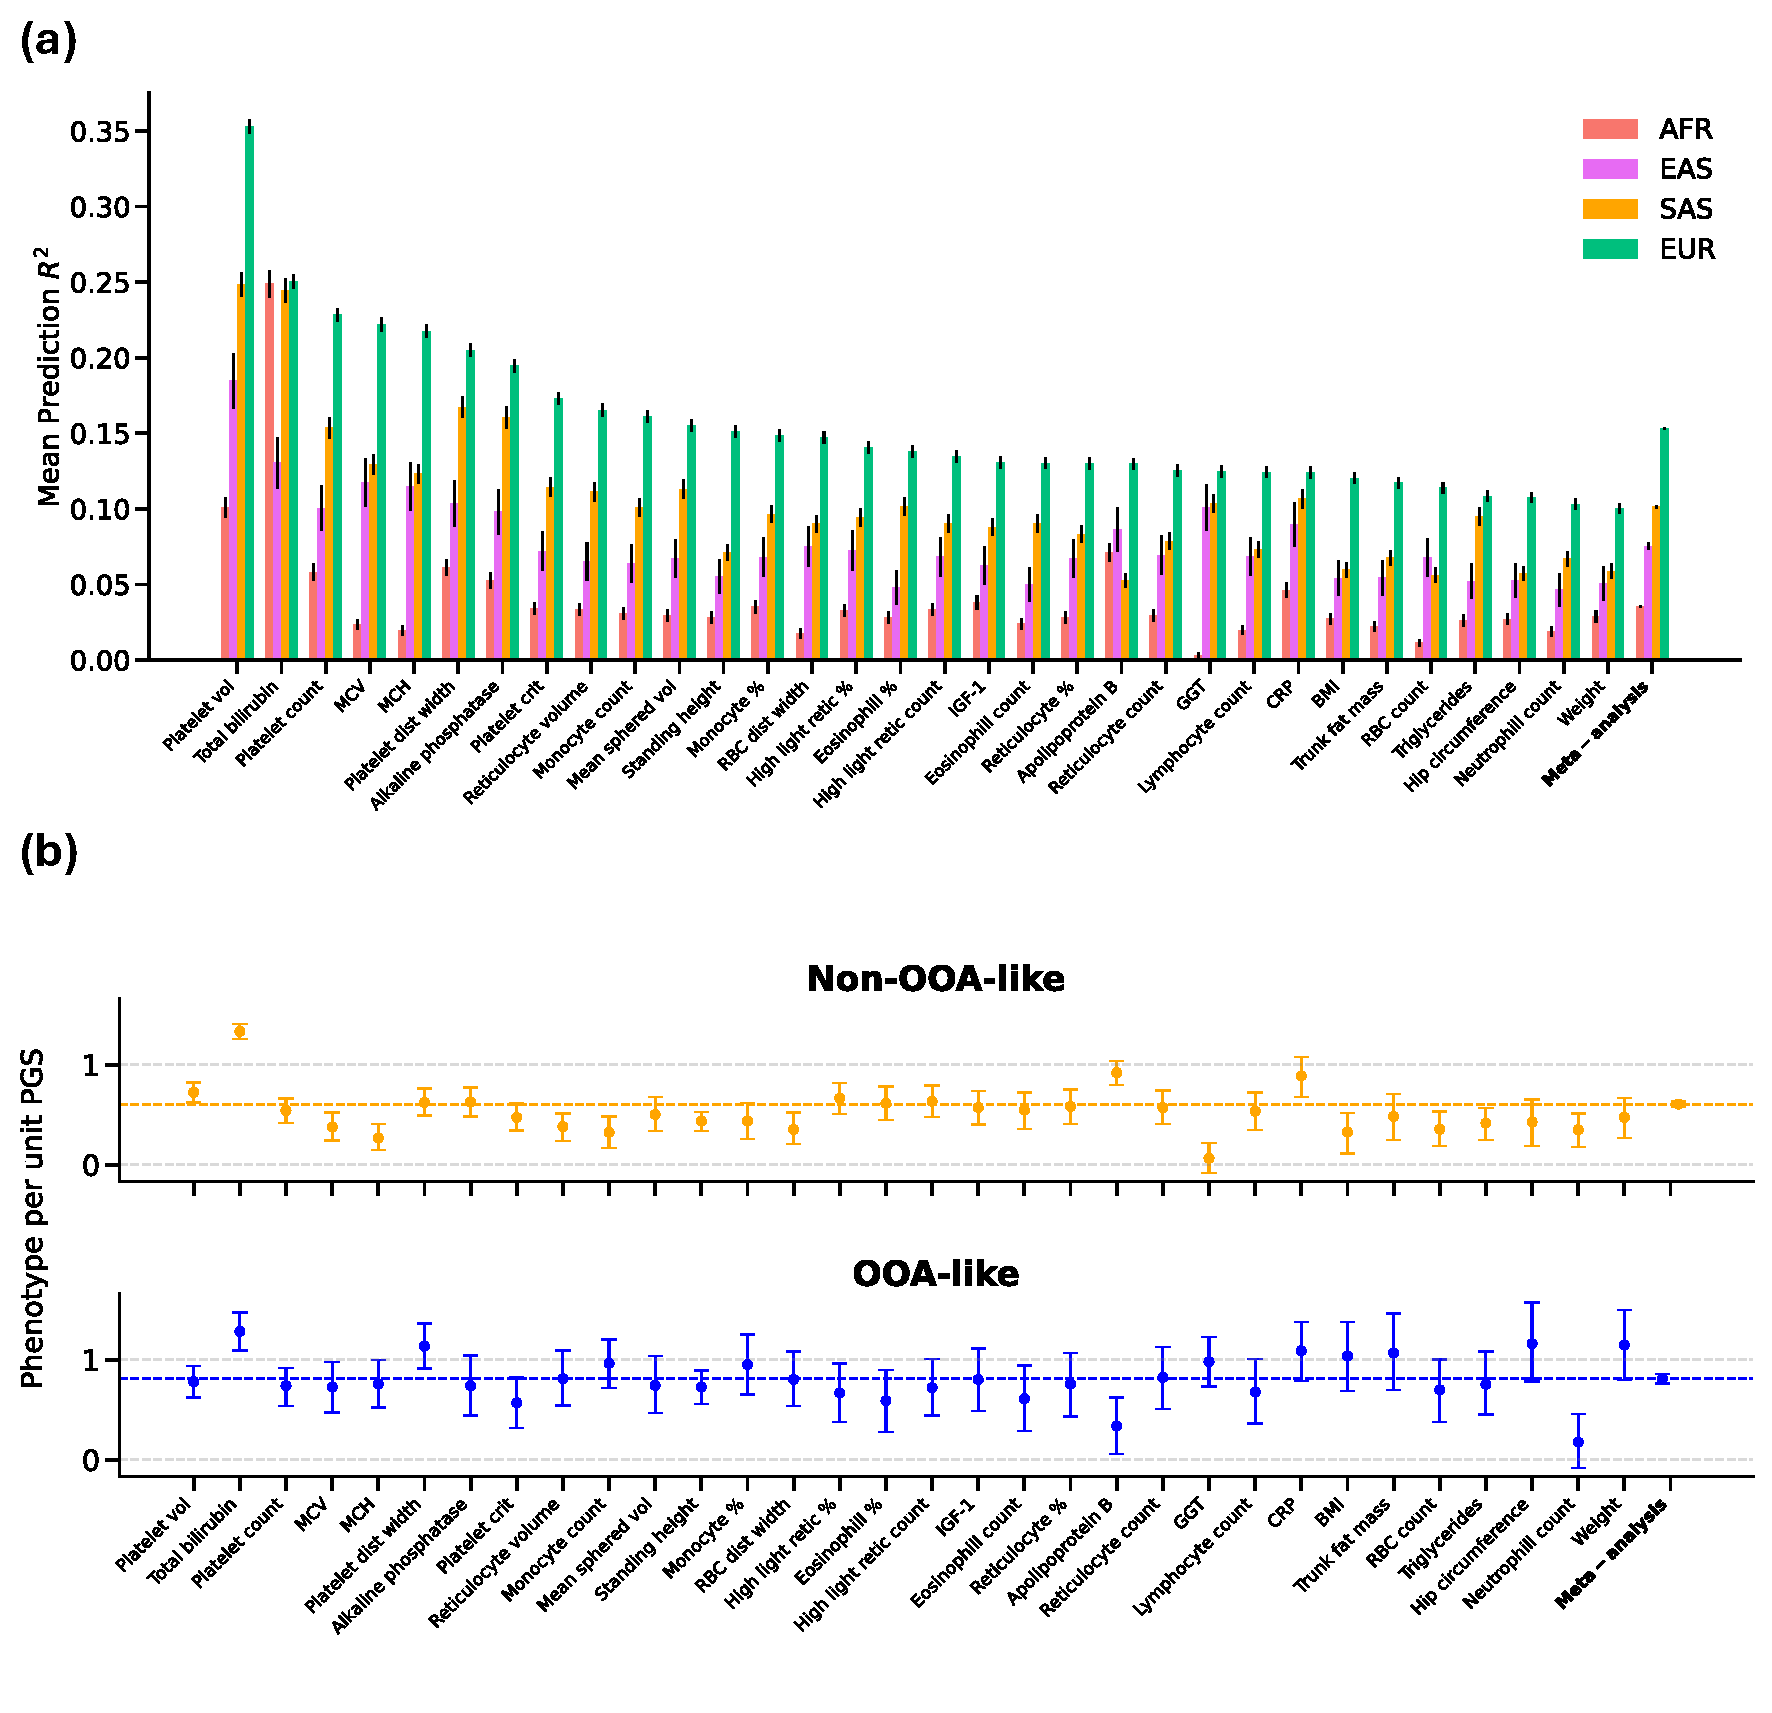
\includegraphics[width=\linewidth]{figures/gb_deepadmix/gb_real_deep_5.pdf}
    \captionsetup{width=\textwidth+3cm}
    \caption{
    \footnotesize
    \textbf{Differences in PGS predictive power across populations and deep admixture components.} (a) PGS prediction $R^2$ across $32$ quantitative phenotypes and four population groups: self-identified non-British Europeans (EUR), South Asians (SAS), East Asians (EAS), and Africans (AFR). Error bars represent the 95\% confidence intervals for the prediction $R^2$. (b) Normalized predictive ability of the PGS based on the OOA-like and non-OOA-like ancestry components across the same $32$ quantitative phenotypes. Error bars represent the 95\% confidence intervals calculated using $1{,}000$ bootstrap replicates. Traits are sorted based on their prediction $R^2$ in Europeans. PGS was calculated using posterior mean effect estimates obtained during Quickdraws' model fitting step. A meta-analysis using inverse variance-weighted average across traits is presented in (a) and (b).
    }
    \label{fig:gb_deepadmix_anchor}
\end{figure}

\clearpage

\section{Discussion}
\label{sec:ch3-discussion}

% Paragraph 1 is Summary/interpretation of major findings + their importance
% Paragraph 2 (optional) is Discussion of other methods
% Paragraph 3 is Implications for downstream analyses
% Paragraph 4 is Limitations and future work

% Genealogies offer a more direct understanding of human past, offering a more interpretable and powerful approach to understand admixture and migration history. 
% In this work we present, GhostBuster a mixture model which leverages the inferred genealogies to understand and infer admixture events in the past.
% GhostBuster offers state-of-the-art power to detect recent and ancient admixture events in simulations and established real-data examples.
% Analyzing recent and ancient events in Africa, we find evidence for widespread back to Africa migration, which has resulted up to 20\% ancestry in some sub-saharan African samples. 
% We validate and characterize this admixture event across different African populations, and find the migration bought with it Neanderthal ancestry explaining the non-zero Neanderthal ancestry in Africans, and elevated TCC to TTC mutation rates.
% We hypothesize the groups contributing this Eurasian ancestry might be associated with present day north Africans, and Anatolian farmers from Europe. 
% We also find evidence for a ancient admixture event between groups with differential coalescence rates with modern-day Eurasians.
% This deep admixture model supports the presence of two ancient populations, where one population resembles the out of Africa population, which migrated out of African and eventually gave rise to Eurasians. 
% We find difference in PGS portability among African samples dependent on this ancestry decomposition. 


Genealogies provide a powerful and interpretable framework for understanding human history. In this work, we introduce GhostBuster, a mixture model that leverages inferred genealogies to detect and analyze historical admixture events. GhostBuster identifies patterns in the coalescence history of target individuals, clustering these patterns to detect ancestry differences across the genome. In simulations involving both modern and ancient gene flow, GhostBuster demonstrated high power for detecting admixture events and provided more accurate local ancestry inference than traditional HMM-based methods \cite{skov2018detecting}. In real data examples, including admixture events within the past $2{,}000$ years, GhostBuster’s results aligned closely with previous haplotype-based methods \cite{salter2019fine}, underscoring its robust capability to detect recent gene flow events.

We applied GhostBuster to investigate the population history of Africa by analyzing joint genealogies inferred from publicly available modern and ancient populations. Our analysis began by focusing on admixture history in the context of back-to-Africa migration \cite{pickrell2012genetic, llorente2015ancient, chen2020identifying}. Using GhostBuster, we uncovered widespread back-to-Africa migration from Eurasia, contributing an average of approximately $2.5\%$ and up to $10\%$ Eurasian ancestry across all present-day African populations analyzed. We identified previously unrecognized ancient back-migration events in several populations, particularly in West and Central Africa, while corroborating previously documented back-migration events in East and South Africa \cite{pickrell2014ancient, llorente2015ancient}. We estimated the timing of these admixture events ranged from the past millennium to approximately $10{,}000$ years ago, coinciding with the end of the last Ice Age and aligning with the Green Sahara period \cite{tierney2017rainfall, larrasoana2013dynamics}, when the Sahara was likely more navigable. Characterizing and validating the admixture event, we also found that this back-migration event alone provides a plausible explanation for the presence of small amounts of Neanderthal ancestry in African genomes. Furthermore, the Eurasian segments in Africans exhibited distinct mutational profiles, including elevated TCC to TTC mutations, and showed genetic proximity to populations in modern-day North Africa, the Middle East, and Anatolian farmer-related groups. These findings suggest a connection between this migration and the spread of farming practices from Europe into Africa.

%Overall, GhostBuster’s ancestry partitioning, further validated by independent validations like Neanderthal ancestry overlap and enriched TCC to TTC mutation rates, provides a clearer and more comprehensive view of the extent and impact of this back-to-Africa migration. 

In addition to the back to Africa migration, we applied GhostBuster to examine deeper population history in Africa, focusing on events from $10{,}000$ years ago and earlier. Previous studies have proposed various hypotheses including presence of ghost populations \cite{skoglund2017reconstructing,durvasula2020recovering}, weak structured stem \cite{ragsdale2023weakly}, and ancient migrations \cite{lipson2020ancient} to explain the complex population structure in sub-Saharan Africa. Using GhostBuster, we identified two distinct ancestral components in the African genome, differentiated by their coalescence rates with Eurasians. We hypothesize that these components reflect an ancient admixture event occurring around or after the out-of-Africa migration, involving two ancestral populations. One of these populations likely represents a group closely related to the out-of-Africa population. We observed significant differences in population sizes and historical hotspot activity between these ancient groups, as evidenced by variations in weak to strong mutation rates across the genome and at specific recombination hotspots. Additionally, we identified differential affinities of the two components with archaic human groups, including Neanderthals and Denisovans, and found evidence of a deep population split between the two components, occurring at least $300{,}000$ years ago. Finally, our analysis of African individuals in the UK Biobank revealed substantial differences in polygenic score (PGS) portability between these two ancestral components when European GWAS data were used for PGS construction.

%This finding emphasizes the importance of ancestry decomposition in PGS analyses, highlighting how deep population structure can shape genetic predictions within African populations.
Overall, GhostBuster proved effective in characterizing previously known admixtures while uncovering new insights into more ancient admixture events in Africa. We believe GhostBuster can be leveraged to investigate a wide range of admixture events, both recent and ancient, offering valuable insights with numerous downstream applications. For instance, admixture inference is crucial for understanding the evolutionary history of species, shedding light on the complex dynamics of migration, adaptation, and gene flow that have shaped modern populations. By inferring local ancestry along the genome, GhostBuster enables the identification of regions involved in adaptive admixture, where genes from one population may confer selective advantages in another. Furthermore, GhostBuster’s ability to detect and analyze fine-scale admixture has significant implications for medical genetics, helping researchers uncover the genetic basis of phenotypic variation across populations, including differences in disease susceptibility and other health-related traits.


\subsection{Limitations and future work}

We identify several current limitations and areas for future improvement. First, GhostBuster uses genome-wide genealogies, which generally requires high-coverage sequencing data to accurately infer genetic relationships between samples. However, many ancient DNA samples are sequenced at low coverage, limiting their integration into current genealogy inference methods. Addressing this challenge through scalable ``threading'' techniques to incorporate low-coverage ancient DNA into genealogies, or through imputation methods \cite{rubinacci2021efficient, sousa2023imputation}, could significantly expand the number of ancient samples available for analysis. This would greatly improve GhostBuster’s capacity to provide a comprehensive view of population history, particularly in cases where admixture signals are subtle and may not be apparent from limited high-coverage ancient DNA or modern samples -- such as in the complex 3-way admixture observed in Europe (see Section \ref{sec:ch2-gb-real-eur}). 

% Second, genomic biases (such as those introduced by background selection) or errors in genealogy inference can occasionally produce false admixture signals. As demonstrated in our simulations (see Section \ref{sec:ch2-gb-sim}), biases during genealogy inference are typically mitigated by evaluating the held-out log-likelihood, assessing confidence in local ancestry inference, and analyzing coancestry curve dating. In contrast, biases along the genome due to background selection or other genomic factors can be identified through admixture dating and examining correlations with metrics of background statistics. Advancements in genealogy inference methods to reduce biases and increase reconstruction accuracy would further strengthen our model's reliability, making this an important direction for future research. 

Second, biases in genealogy inference can occasionally produce false admixture signals, as shown in our simulations (see Section \ref{sec:ch2-gb-sim}). Typically, these biases are mitigated by evaluating the held-out log-likelihood, assessing confidence in local ancestry inference, and analyzing coancestry curve dating. Advancements in genealogy inference methods to reduce biases and increase reconstruction accuracy would further strengthen our model’s reliability, making this an important direction for future research.


Third, GhostBuster is computationally slower than some other ancestry inference software that rely on low-dimensional summary statistics. While these alternatives often lack the statistical power to detect subtle admixture signals, there are promising strategies to improve GhostBuster’s computational efficiency. For instance, using PCA on the coalescence count matrix generated by GhostBuster can provide a fast, approximate inference of admixture. Additionally, implementing GhostBuster in a low-level programming language or leveraging modern computing architectures like GPUs could significantly improve its speed, making it more feasible for large-scale analyses. We propose these improvements as directions for future work. Finally, expanding the use of GhostBuster to study the evolutionary history of other species would also be highly beneficial. In the next section, we demonstrate its effectiveness in uncovering an admixture event in American wolves. We believe that GhostBuster could similarly aid in understanding the population dynamics and admixture history of several other species, paving the way for broader applications in evolutionary biology. 

% - Low coverage ancients and threading
% - sampling from the genealogies to increase robustness to errors
% - Depends on labelling of reference populations 
% - Choosing number of components needs more work

\subsection{Understanding admixtures in non human organisms}

To demonstrate the ability of GhostBuster to detect admixture beyond humans, we applied it to understand the admixture history of North American wolves. We analyzed five American Great Lakes wolves alongside one Coyote and 29 European grey wolf genomes. Previous research has shown that Great Lakes wolves have undergone admixture with Coyotes over the last few thousand years \cite{lehman1991introgression,bozarth2011coyote,vonholdt2016whole}. We used the Relate trees and dataset from \cite{bergstrom2022grey}, along with a canid recombination map from \cite{auton2013genetic}. GhostBuster was run with two components, considering coalescence events over a wide time interval ranging from $100$ years to one million years. Our analysis revealed that the major component, contributing approximately around three quarters, was closer to grey wolves, while the minor component was closer to the coyote sample in the dataset. Using coancestry curve fitting, we identified the two-date admixture model as the best fit for the observed coancestry curves. The inferred admixture dates were $186.7$ generations ($560.1$ years) and $1777.7$ generations ($5{,}333.1$ years), with $79$\% of the observed admixture attributed to the older admixture date. See Figure \ref{fig:gb_real_wolves} for further details.

\begin{figure}[h!]
    \centering
    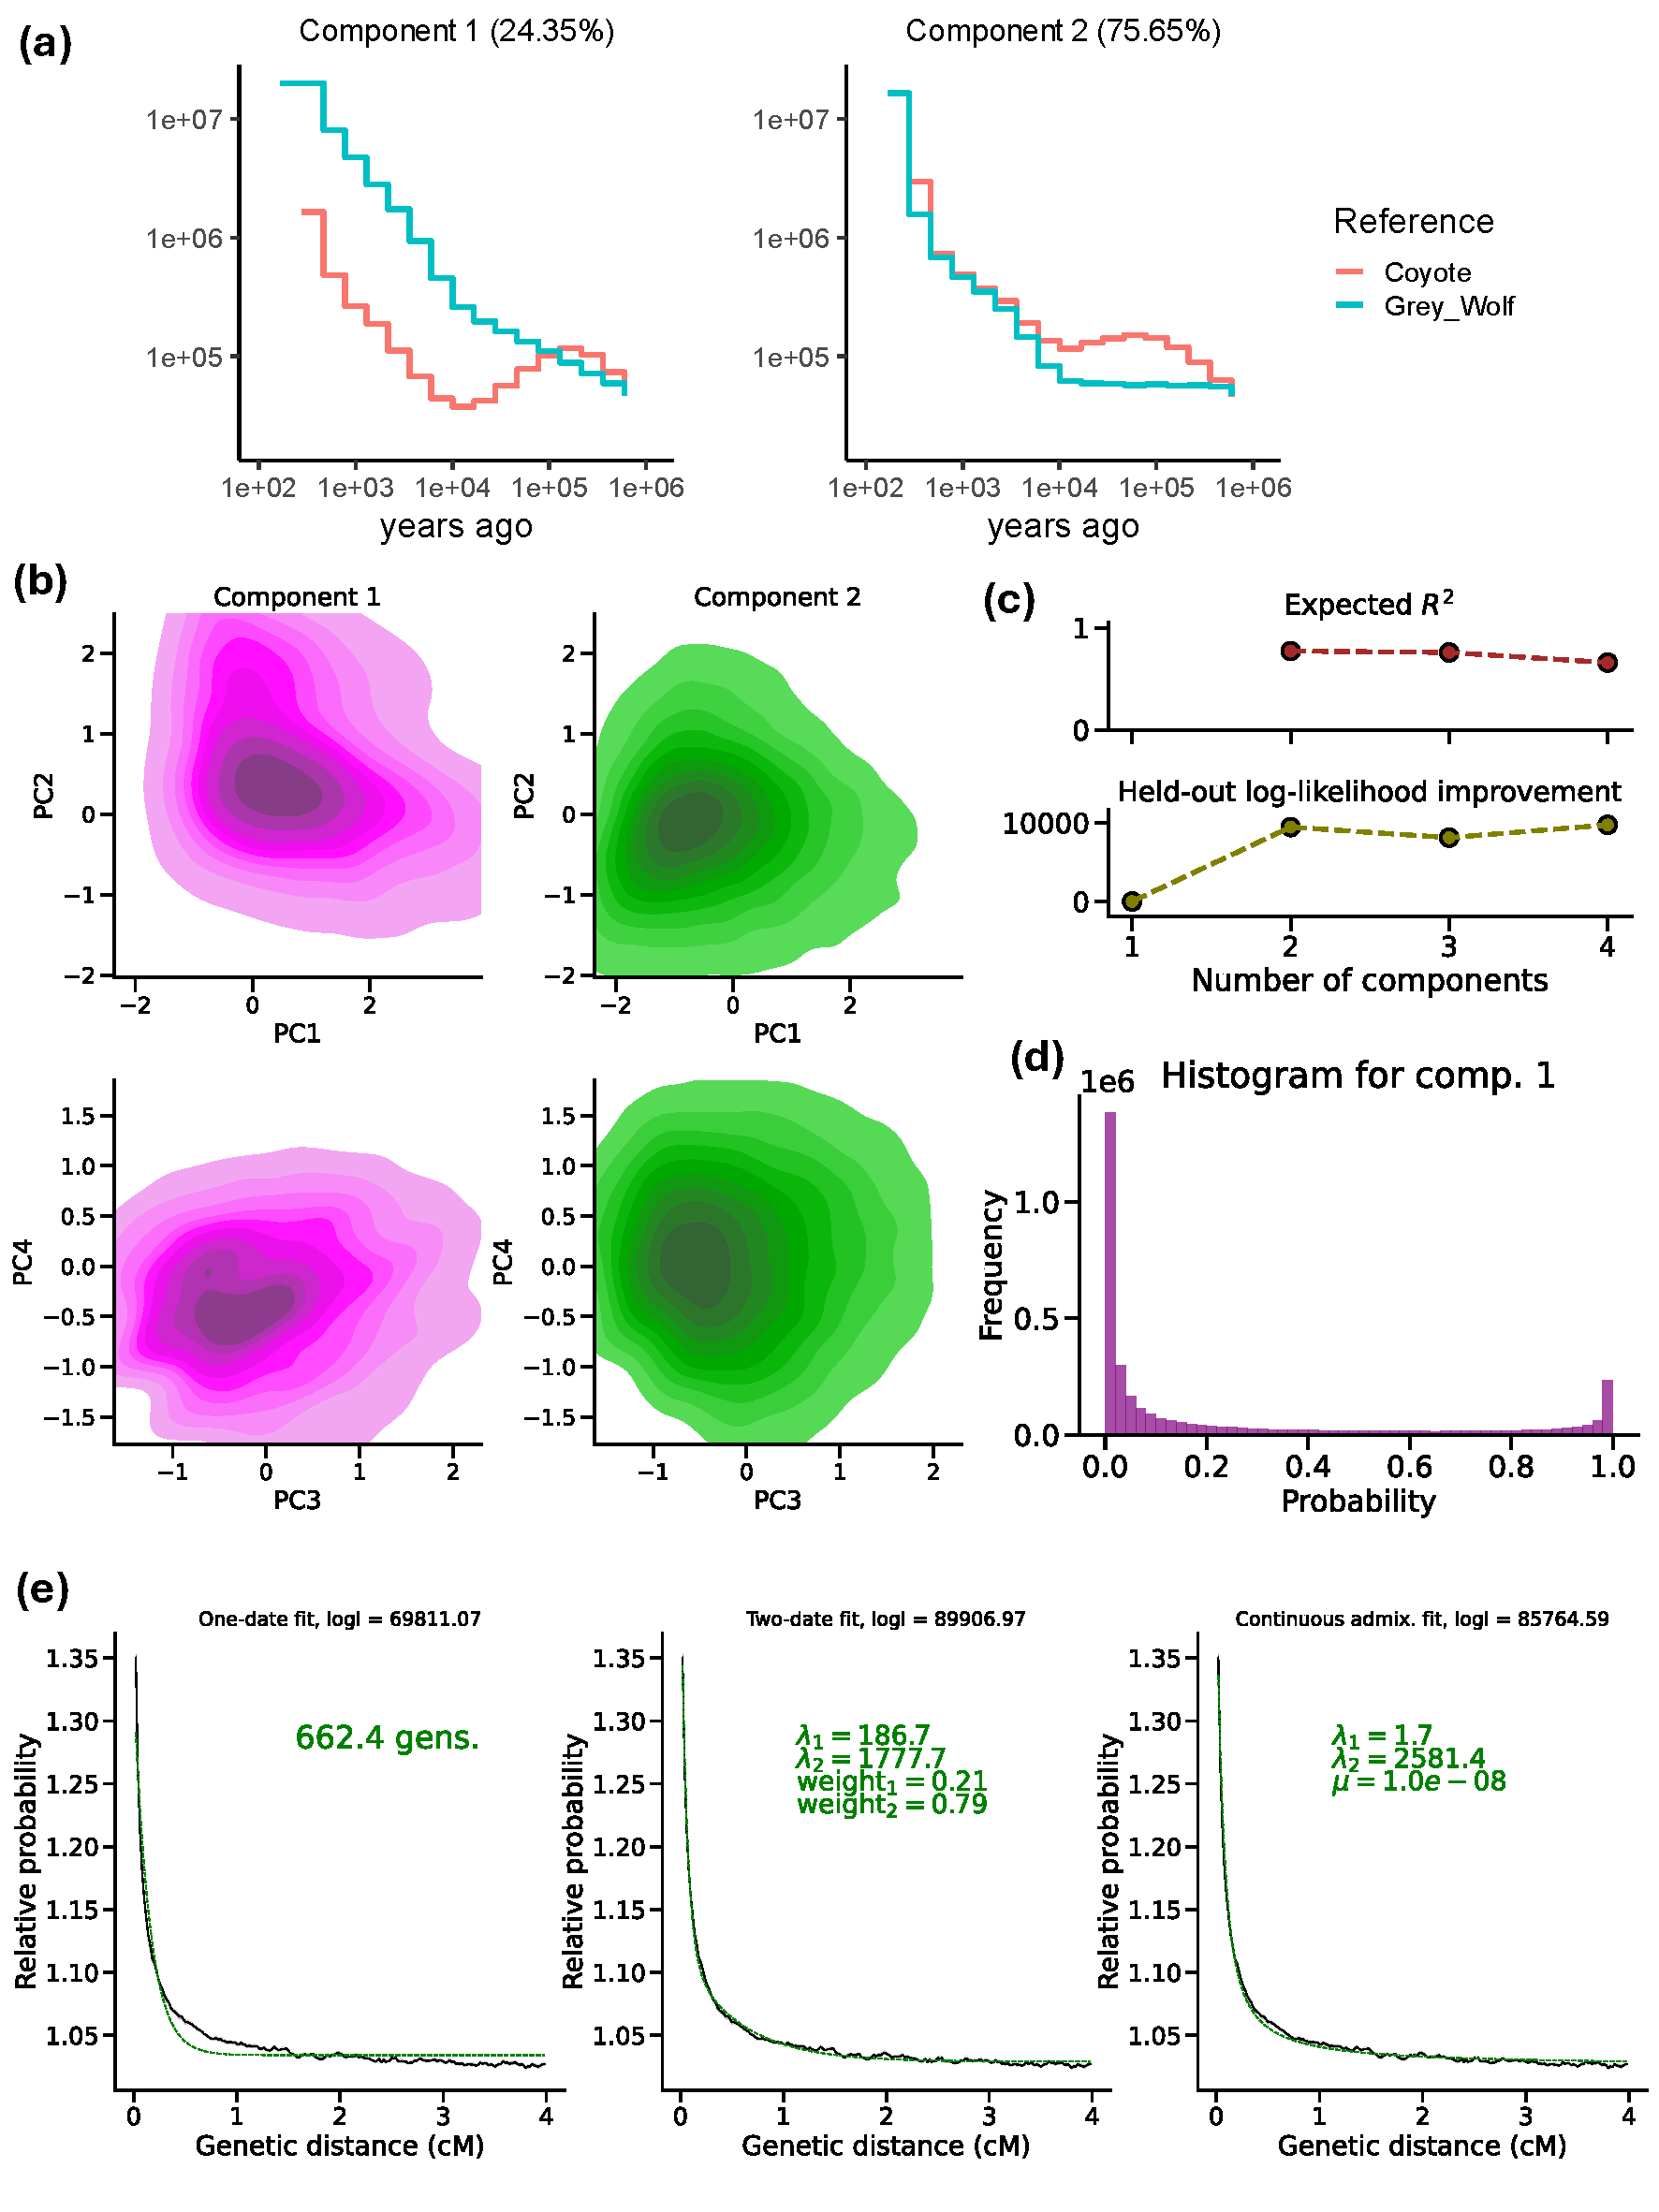
\includegraphics[width=\linewidth]{figures/gb_sims/gb_real_wolves.pdf}
    \captionsetup{width=\textwidth+3cm}
    \caption{
    \footnotesize
    \textbf{Decomposing American wolves with grey wolves and coyote as reference.} (a) Inferred inverse coalescence rates and proportions: each line represents inverse coalescence rate profiles with a reference population. (b) PCA visualization of the coalescence count and opportunity matrix derived from the genealogies plotted separately for each component. (c) Expected coefficient of determination and held-out log-likelihood improvement with varying number of components. (d)  Histogram of the inferred local ancestry posteriors. (e) Coancestry curves and model fit for one-date, two-date, and continuous migration scenarios (admixture dates in generations). The figure title includes `logl', which refers to the log-likelihood of the fit (higher values indicate a better fit). The PCA visualization in (b) is based on a KDE plot with a threshold of 0.05, and binary local ancestry estimates are obtained by thresholding the inferred posteriors at 0.5.
    }
    \label{fig:gb_real_wolves}
\end{figure}